\documentclass[a4paper,oneside ,14pt]{extreport}

\usepackage[T2A]{fontenc} 
\usepackage[utf8]{inputenc}
\usepackage[english,russian]{babel}
\usepackage[unicode, pdftex]{hyperref}
\usepackage{amsmath}
\usepackage{vmargin}
\usepackage{fancyvrb}
\usepackage{indentfirst}
\setmarginsrb{2cm}{1.5cm}{1cm}{1.5cm}{0pt}{0mm}{0pt}{13mm}
\usepackage{indentfirst}
\usepackage{graphicx}
\usepackage{booktabs} 
\usepackage{polynom}
\usepackage{setspace}
\usepackage{multirow}
\usepackage{caption}   % Изображение сноски
\usepackage{graphicx}  
\usepackage{caption}
\usepackage{subfigure} % Пакет подкарты
\usepackage{listings}
\usepackage[LGRgreek]{mathastext}
\usepackage{tikz}                   % Продвинутый пакет векторной графики
\usepackage{tikz-3dplot}
\usetikzlibrary{chains}             % Для примера tikz рисунка
\usetikzlibrary{shapes.geometric}   % Для примера tikz рисунка
\usetikzlibrary{shapes.symbols}     % Для примера tikz рисунка
\usetikzlibrary{arrows}             % Для примера tikz рисунка
\usepackage{pgfplots}
\pgfplotsset{compat=1.18}
\usetikzlibrary{pgfplots.colorbrewer}
\usetikzlibrary{pgfplots.colorbrewer}
\usetikzlibrary{pgfplots.polar}
\usetikzlibrary{angles, arrows.meta, quotes}
\usepackage{siunitx}
\usepackage{cite}
\usepackage{setspace}
\usepackage{gnuplottex}

\onehalfspace
\pgfplotsset{cycle list/Dark2, cycle list/Set1}
\pgfplotsset{
    % create custom style and add all keys/options that are valid for this
    % particular style
    RCS Plot/.style={
        %        height=0.4\textwidth,
        width=\textwidth,
        minor tick num = 4,
        enlarge x limits = 0,
        grid=major,
        xlabel near ticks,
        ylabel near ticks,
        legend pos = north west,
        legend style={font={\tiny}},
        mark=none,
        thin,
        line join=bevel,
        cycle list name=Dark2,
        font={\footnotesize}
    },
}

%opening
\author{Александр Пахмутов}
\title{Практическое руководство по проектированию цифровых устройств на ПЛИС}
\date{\today}

\newcommand{\compconj}[1]{%
  \overline{#1}%
}

\begin{document}

\maketitle
\thispagestyle{empty} 
\newpage 

\tableofcontents{}

\newpage

\chapter{Лабораторная работа №1. Реализация комбинационных логических элементов}

В данной лабораторной работе будут рассмотрены базовые навыки работы в САПР Vivado, такие как: создание нового проекта и 
его настройка, создание HDL-файлов, создание файлов ограничений(xdc), запуск генерации конфигурационного файла и его загрузка в ПЛИС.
Кроме того рассмотрим реализацию простейших комбинационных логических элементов на языке Verilog.

\section{Основы работы в САПР Vivado}

\subsection{Шаг 1: создаём проект}

\begin{figure}[!ht]
	\centering
	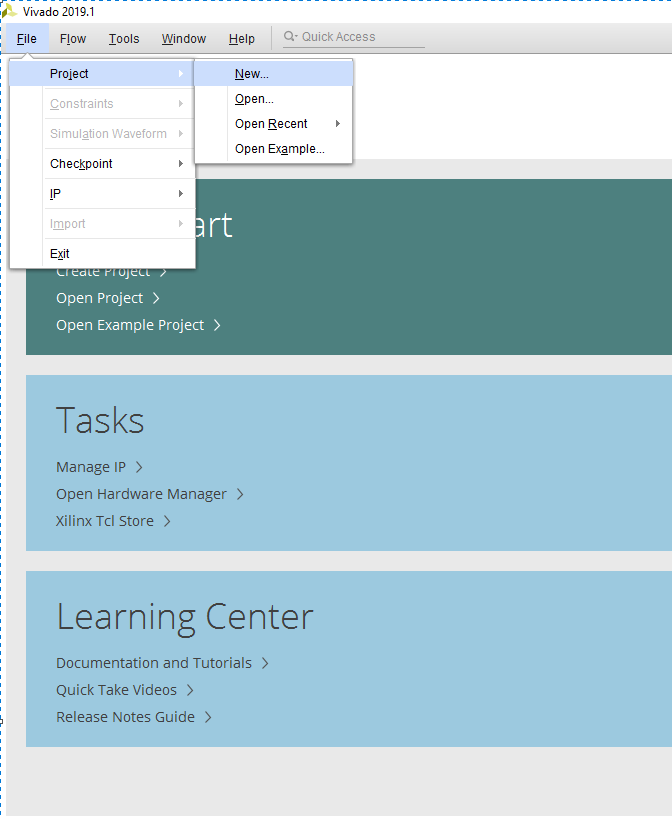
\includegraphics[width=0.3\textwidth]{image/m_3.png}
	\caption{Создание нового проекта в Vivado}
	\label{l1_new_prj}
\end{figure}

\begin{figure}[!ht]
	\centering
	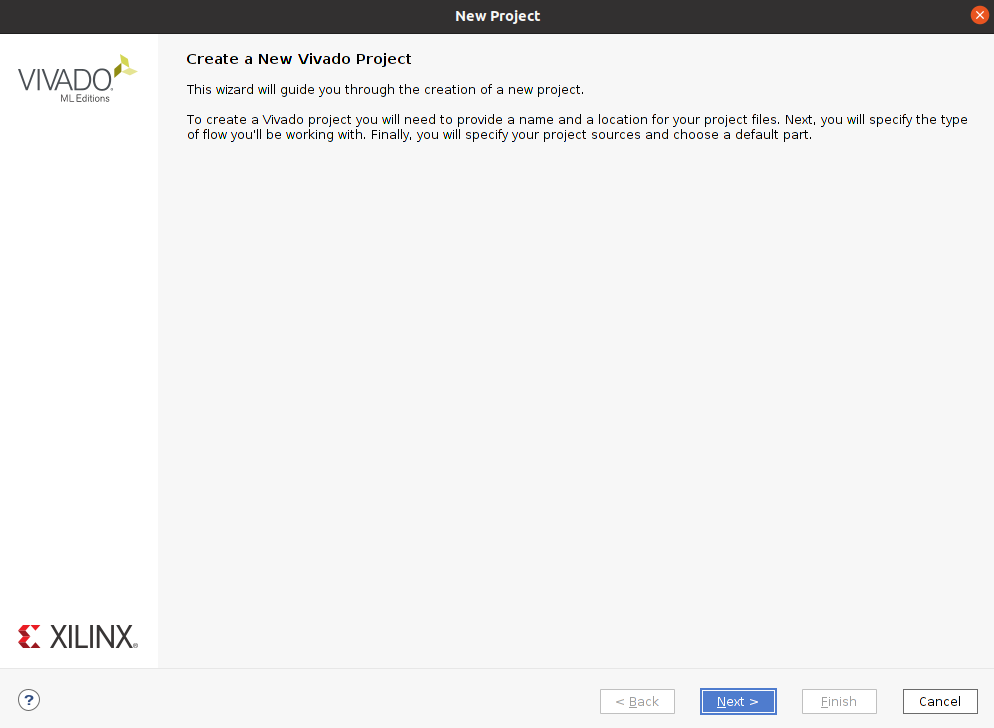
\includegraphics[width=0.4\textwidth]{image/2}
	\caption{Окно мастера создания нового проекта}
	\label{l1_master}
\end{figure}

Для создания проекта щелкните «File->Project->New» на панели быстрого запуска, как показано на рисунке ~\ref{l1_new_prj}. Откроется диалоговое окно «New project», как показано на рисунке ~\ref{l1_master}. Нажмите «Next», чтобы продолжить.

\newpage

\begin{figure}[!ht]
	\centering
	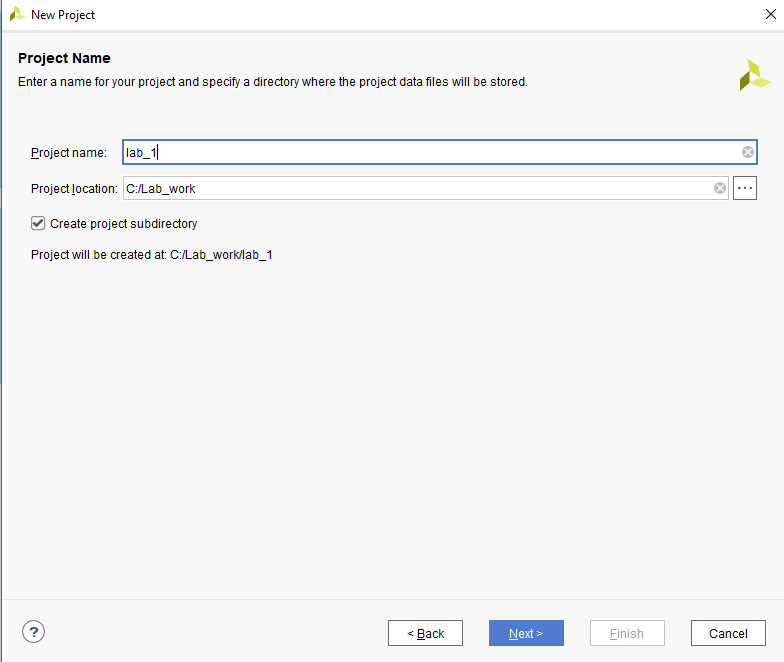
\includegraphics[width=0.4\textwidth]{image/l1_lab_1}
	\caption{Название проекта, путь к проекту}
	\label{l1_name}
\end{figure}
Введите название проекта, как показано на рисунке~\ref{l1_name}. Обычно рекомендуется сделать название проекта более информативным, чтобы вам было легче идентифицировать свои проекты в будущем. Например, если вы разрабатываете семисегментный контроллер, вы можете назвать проект «Семисегментный контроллер». Вам следует избегать использования пробелов в имени или расположении проекта, потому что пробелы могут привести к сбою некоторых инструментов.

\begin{figure}[!ht]
	\centering
	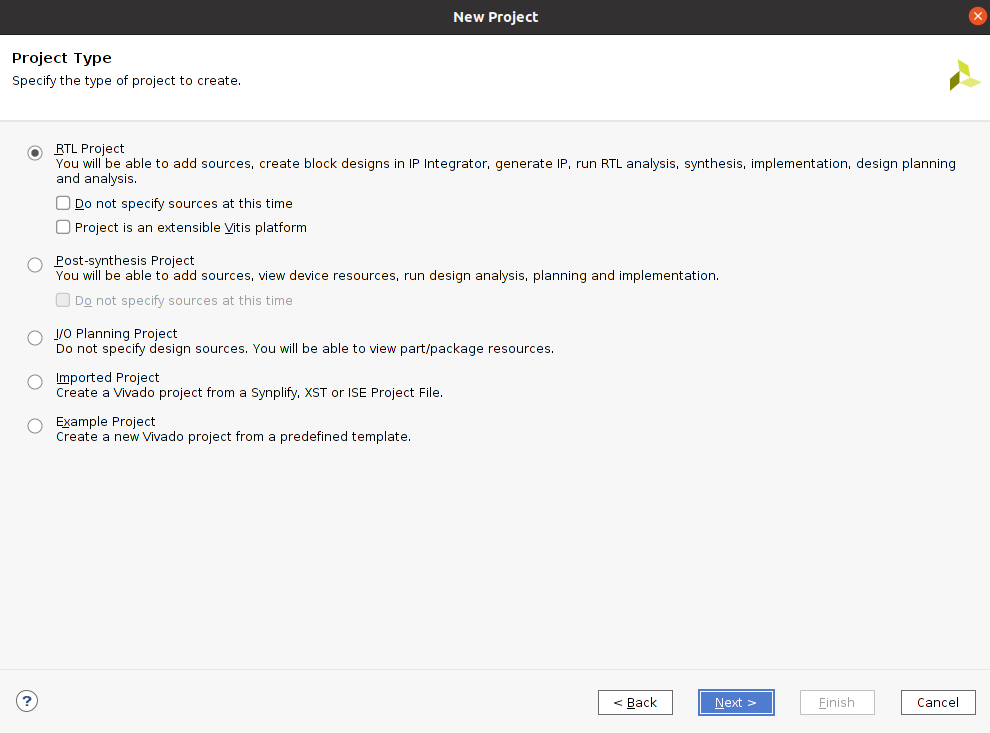
\includegraphics[width=0.4\textwidth]{image/8}
	\caption{Выбор типа создаваемого  проекта}
	\label{l1_type_prj}
\end{figure}

«Project Type» настраивает определенные инструменты дизайна и внешний вид IDE в зависимости от типа проекта, который вы собираетесь создать. В большинстве случаев вы выбираете «RTL Project»,чтобы настроить инструменты для создания нового дизайна, как показано на рисунке ~\ref{l1_type_prj}.

\begin{figure}[!ht]
	\centering
	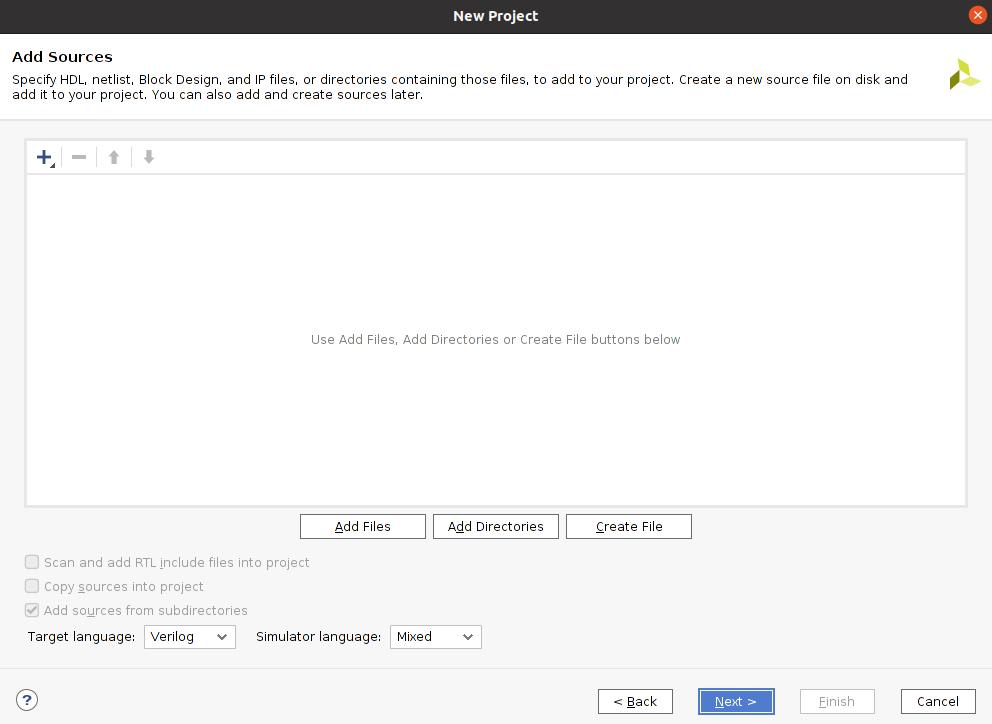
\includegraphics[width=0.4\textwidth]{image/9}
	\caption{Подключение исходных файлов}
	\label{l1_source}
\end{figure}

В новом дизайне вы не добавляете какие-либо существующие источники, потому что вы их еще не создали.

На данный момент нет существующих источников для добавления, поэтому просто нажмите «Next» (см. рис. ~\ref{l1_source}).

\begin{figure}[!ht]
	\centering
	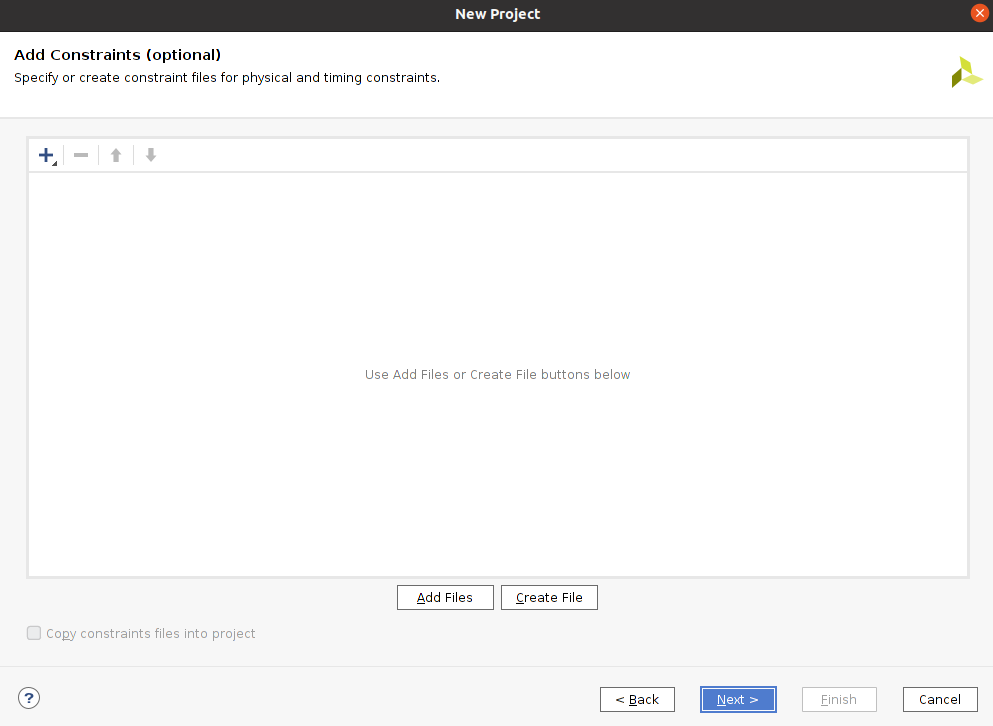
\includegraphics[width=0.4\textwidth]{image/10}
	\caption{Подключение .xdc файлов}
	\label{l1_xdc}
\end{figure}

Файлы ограничений предоставляют информацию о физической реализации проекта. 

Позже в этом руководстве вы создадите файл ограничений, чтобы определить, какие именованные узлы схемы должны быть подключены к каким физическим контактам. Но на данный момент у вас нет существующего файла ограничений для добавления, поэтому вы можете просто нажать «Next»(см. рис. ~\ref{l1_xdc}).

\begin{figure}[!ht]
	\centering
	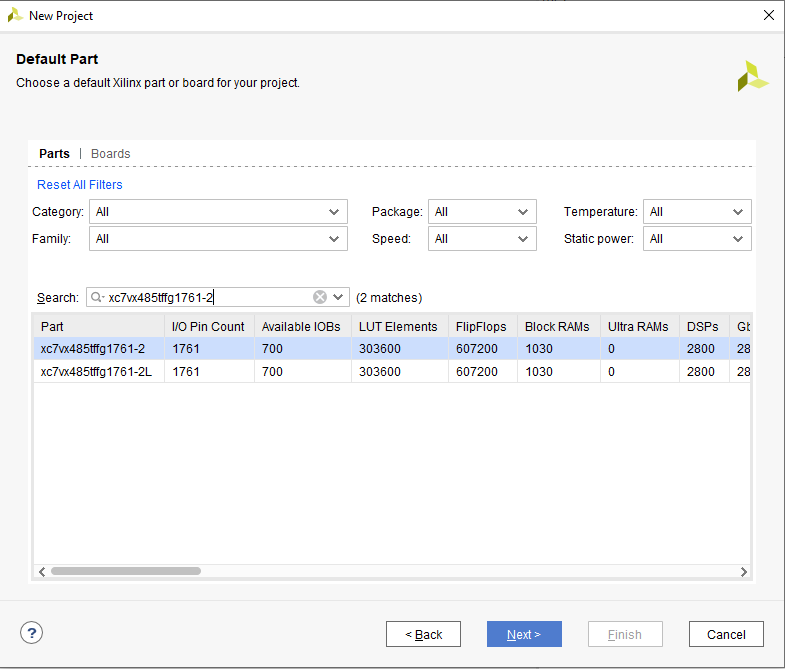
\includegraphics[width=0.4\textwidth]{image/m_9.png}
	\caption{Выбор FPGA}
	\label{l1_fpga}
\end{figure}

Xilinx производит множество различных ПЛИС, и синтезатору необходимо точно знать, какую вы используете, чтобы он мог создать корректную прошивку. На отладочной плате VC707 установлена \verb|xc7vx485tffg1761-2|. Выберете ПЛИС, как показано на рисунке ~\ref{l1_fpga}.

\begin{figure}[!ht]
	\centering
	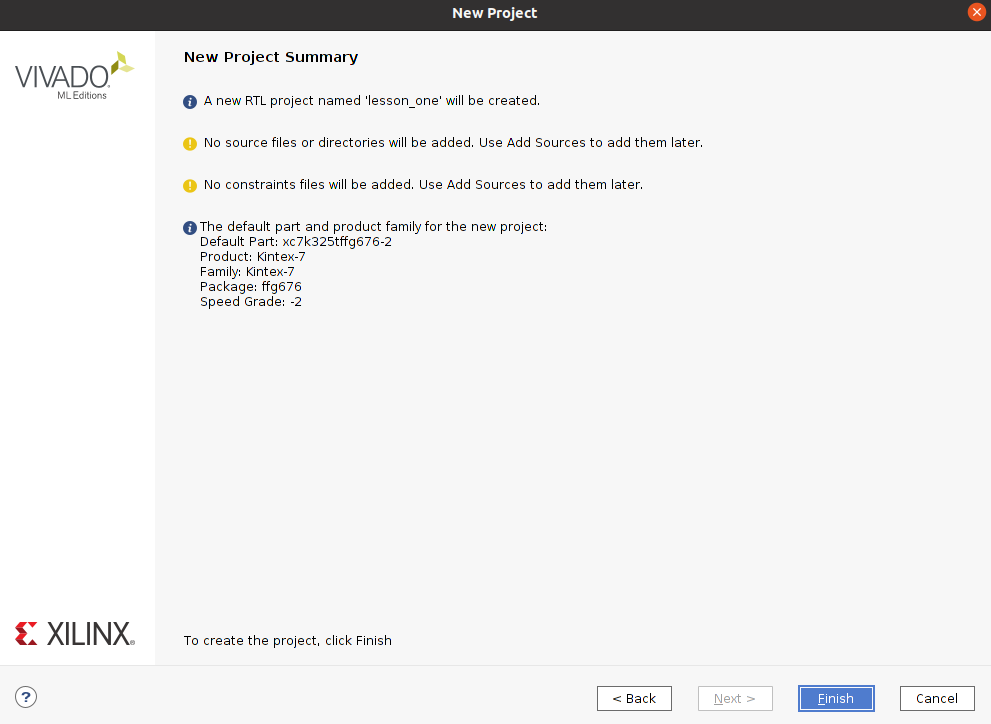
\includegraphics[width=0.4\textwidth]{image/summary}
	\caption{Cуммарные сведения о создаваемом проекте}
	\label{l1_sum}
\end{figure}

На последней странице мастера создания проекта отображается сводка конфигурации проекта. Убедитесь, что вся информация в сводке верна, и, в частности, убедитесь, что выбрана правильная часть FPGA. Если что-то не так, нажмите назад и исправьте; в противном случае нажмите Готово, чтобы завершить создание пустого проекта. Cуммарные сведения о создаваемом проекте представлены на рисунке ~\ref{l1_sum}.

\subsection{Шаг 2: создаём исходные файлы проекта}

\begin{figure}[htbp]	
	\subfigure[Схема подключения светодиодов к ПЛИС] 
	{
		\begin{minipage}{8cm}
			\centering         
			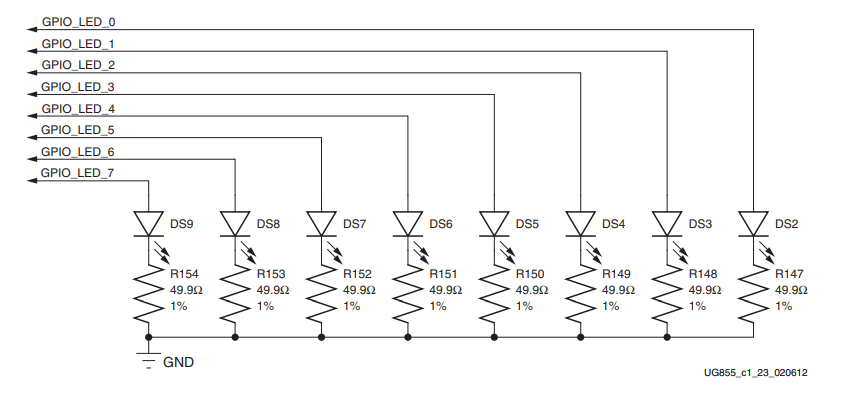
\includegraphics[scale=0.4]{image/LEDS.png}
			\label{LEDS}
		\end{minipage}
	}
	\subfigure[Схема подключения кнопок к ПЛИС] 
	{
		\begin{minipage}{8cm}
			\centering      
			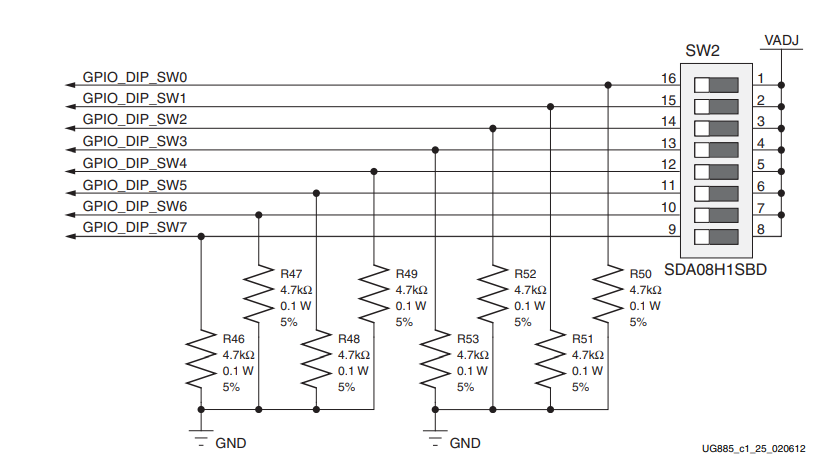
\includegraphics[scale=0.4]{image/DIP_SWITCH.png}
			\label{DIP_SWITCH}
		\end{minipage}
	}
	\caption{Схемы подключения светодиодов и кнопок к ПЛИС} %  %Имя большого изображения
\end{figure}

\begin{figure}[!ht]
	\centering
	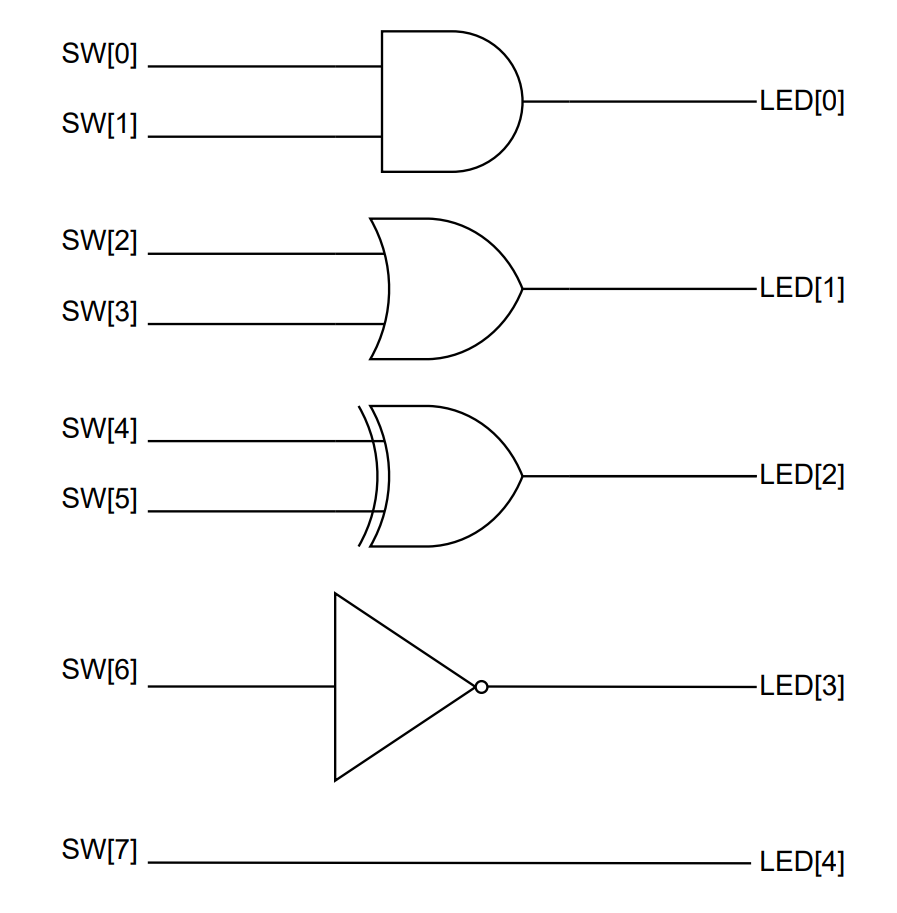
\includegraphics[width=0.3\textwidth]{image/module_0.png}
	\caption{Схема реализуемого модуля}
	\label{module_0}
\end{figure}

Для всех проектов требуются как минимум два типа исходных файлов - файл HDL (Verilog или VHDL) для описания схемы и файл ограничений, чтобы предоставить синтезатору информацию, необходимую для сопоставления вашей схемы с целевой микросхемой.

После создания исходного файла Verilog его можно смоделировать напрямую. Моделирование (более подробно обсуждается позже) позволяет вам работать с компьютерной моделью схемы, поэтому вы можете проверить ее поведение, прежде чем тратить время на ее реализацию на физическом устройстве. Симулятор позволяет вам управлять всеми входами схемы с различными шаблонами с течением времени и проверять, что выходы ведут себя должным образом во всех условиях.

В первой лаборатоной работе вам предоставлены исходные Verilog файл и файл ограничений. Вместо того, чтобы создавать их самостоятельно, как это обычно бывает, вы можете просто скопировать их в пустые исходные файлы или загрузить напрямую в свой проект. В более поздних проектах вы создадите эти файлы самостоятельно.

В данной лабораторной работе будет реализован простейший проект подключения кнопок к светодиодам через логические вентили. Схема электрическая принципиальная подключения светодиодов и кнопок представлены соотвественно на рисунках ~\ref{LEDS}, ~\ref{DIP_SWITCH}. Схема реализуемого модуля представлена на рисунке ~\ref{module_0}.

\subsubsection{Создание HDL-файлов}

\begin{figure}[htbp]	
	\subfigure[Add sources] 
	{
		\begin{minipage}{8cm}
			\centering         
			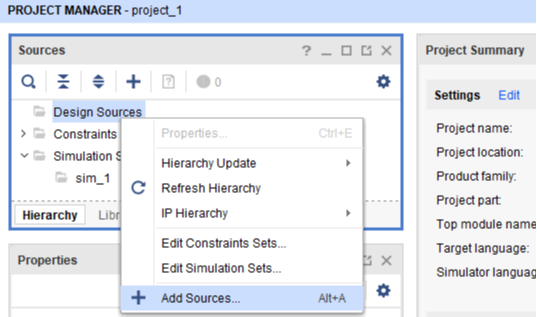
\includegraphics[scale=0.4]{image/l_1_sources.png}   
			\label{add_source_0}
		\end{minipage}
	}
	\subfigure[Окно мастера подключения нового файла] 
	{
		\begin{minipage}{8cm}
			\centering      
			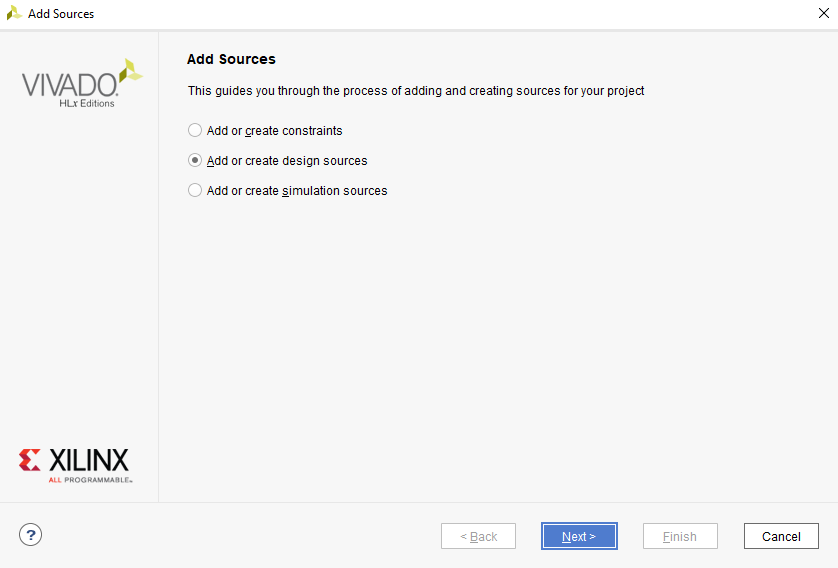
\includegraphics[scale=0.3]{image/l_2_sources.png}   
			\label{add_source_1}
		\end{minipage}
	}
	\caption{Окно мастера подключения нового файла: внешний вид} %  %Имя большого изображения
\end{figure}


\begin{figure}[htbp]	
	\subfigure[Назначаем файлу имя] 
	{
		\begin{minipage}{8cm}
			\centering         
			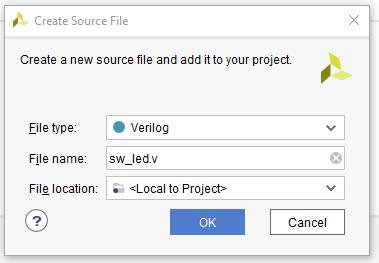
\includegraphics[scale=0.6]{image/sw_led.png}   
			\label{add_source_2}
		\end{minipage}
	}
	\subfigure[Результаты добавления файла] 
	{
		\begin{minipage}{8cm}
			\centering      
			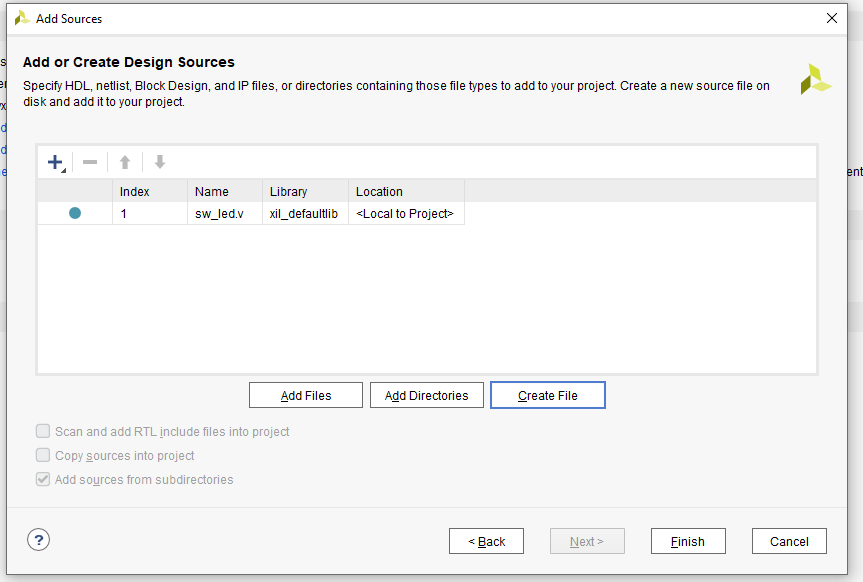
\includegraphics[scale=0.4]{image/sw_led_2.png}   
			\label{add_source_3}
		\end{minipage}
	}
	\caption{Окно мастера подключения нового файла: имя и результаты} %  %Имя большого изображения
\end{figure}

Чтобы создать исходный файл Verilog для вашего проекта, щелкните правой кнопкой мыши «Design Sources» на панели «Sources» и выберите «Add sources»(см. рис. ~\ref{add_source_0}). Появится диалоговое окно «Add sources», как показано на рисунке ~\ref{add_source_1} - выберите «Add or create design sources» и нажмите «Далее».

В диалоговом окне «Add or Create Design Sources» нажмите «Create File», введите имя файла \verb|sw_led| и нажмите «ОК»(см. рис. ~\ref{add_source_2},~\ref{add_source_3}). Вновь созданный файл появится в списке, как показано на рисунке. Нажмите Finish, чтобы перейти к следующему шагу.

Откроется диалоговое окно «define module» и представляет собой область, в которой вы можете определить входные и выходные порты для вашей схемы. В более поздних проектах, если вы введете здесь имена портов, Vivado создаст исходный файл Verilog с уже определенными портами. Для этого упражнения предоставляется полный исходный файл, поэтому вы можете пропустить этот шаг, нажав OK (а затем YES), чтобы продолжить.

Теперь вы увидите, что \verb|sw_led| указан в папке «Design Sources» на панели «Sources». Дважды щелкните \verb|sw_led|, чтобы открыть файл, и замените содержимое (скопируйте и вставьте) приведенным ниже кодом.

\begin{Verbatim}[tabsize=4]
`timescale 1ns / 1ps

module sw_led(
    input wire [7:0] sw,
    output wire [7:0] led
);

    assign led[0] = sw[0] & sw[1];
    assign led[1] = sw[2] | sw[3];
    assign led[2] = sw[4] ^ sw[5];
    assign led[3] = ~sw[6];
    assign led[4] = sw[7];
    assign led[5] = 1'b0;
    assign led[6] = 1'b1;
    assign led[7] = 1'b0;
    
endmodule
\end{Verbatim}

Начнём рассмотрение языка Verilog. Основой описания на Verilog явяляется модуль, представляемый в виде отдельного файла с расширенией .v. 
Структура модуля на языке Verilog имеет следующий вид:

\begin{Verbatim}[tabsize=4]
`timescale 1ns/1ps

module <имя> #(
	[параметры]
)
(
	<объявление портов>
);
[объявление локальных сигналов и переменных]
<синтезируемые конструкции>
endmodule

\end{Verbatim}

Существует три типа портов: вход(input), выход(output), двунаправленный вывод(inout).

Директива `'timescale предназначена для задания временных интервалов моделирования. Первый из них задаёт длительность единицы времени по умолчанию для моделирования.
Второй параметр задаёт величину дискретного шага, используемого средствами моделирования.

Рассмотри реализацию данного модуля. Он соединяет восемь переключателей со светодиодами через логические вентили И, ИЛИ, Исключающее ИЛИ, НЕ. 
Тип порта кнопок объявлен как входной(input), а светодиодов выходной(output). При этом заметим, что порты содержат не один провод, а целую шину - множество проводов, в данном случае по восемь штук. Используя оператор непрерывного присваивания \verb|assign| подключаем кнопки к светодиодам через логические вентили. На оставшиеся светодиоды \verb|led[5], led[6], led[7]| подключим логический ноль, логическую единицу, логический ноль соответственно.

Рассмотрим подробнее синтаксис и свойства оператора непрерывного назначения \verb|assign|.  Синтаксис имеет следующий вид:

\begin{Verbatim}[tabsize=4]
assign #(delay) net_name = expression;
\end{Verbatim}

Оператор непрерывного назначения \verb|assign| функционирует следующим образом. При любом изменении любого из значений в выражении expression с правой стороны, заново вычисляется выражение 
expression и полученное значение по истечении времени, определяемого задержкой delay, присваивается величине слева от знака =.

\subsubsection{Создание файлов ограничений}

\begin{figure}[htbp]	
	\subfigure[Назначаем файлу ограничений имя] 
	{
		\begin{minipage}{8cm}
			\centering         
			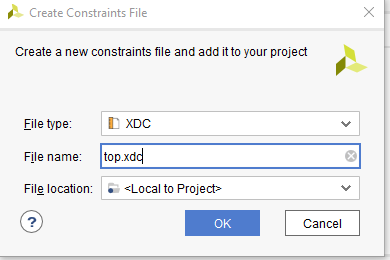
\includegraphics[scale=0.6]{image/xdc.png}   
			\label{add_xdc}
		\end{minipage}
	}
	\subfigure[Результаты добавления файла ограничений] 
	{
		\begin{minipage}{8cm}
			\centering      
			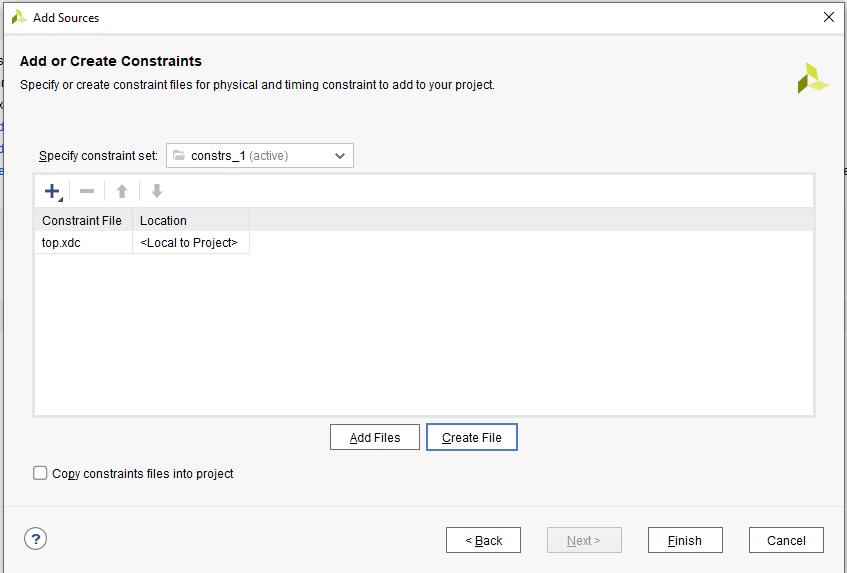
\includegraphics[scale=0.4]{image/xdc_2.png}   
			\label{add_xdc_0}
		\end{minipage}
	}
	\caption{Окно мастера подключения нового файла: имя и результаты} %  %Имя большого изображения
\end{figure}{}

\begin{figure}[!ht]
	\centering
	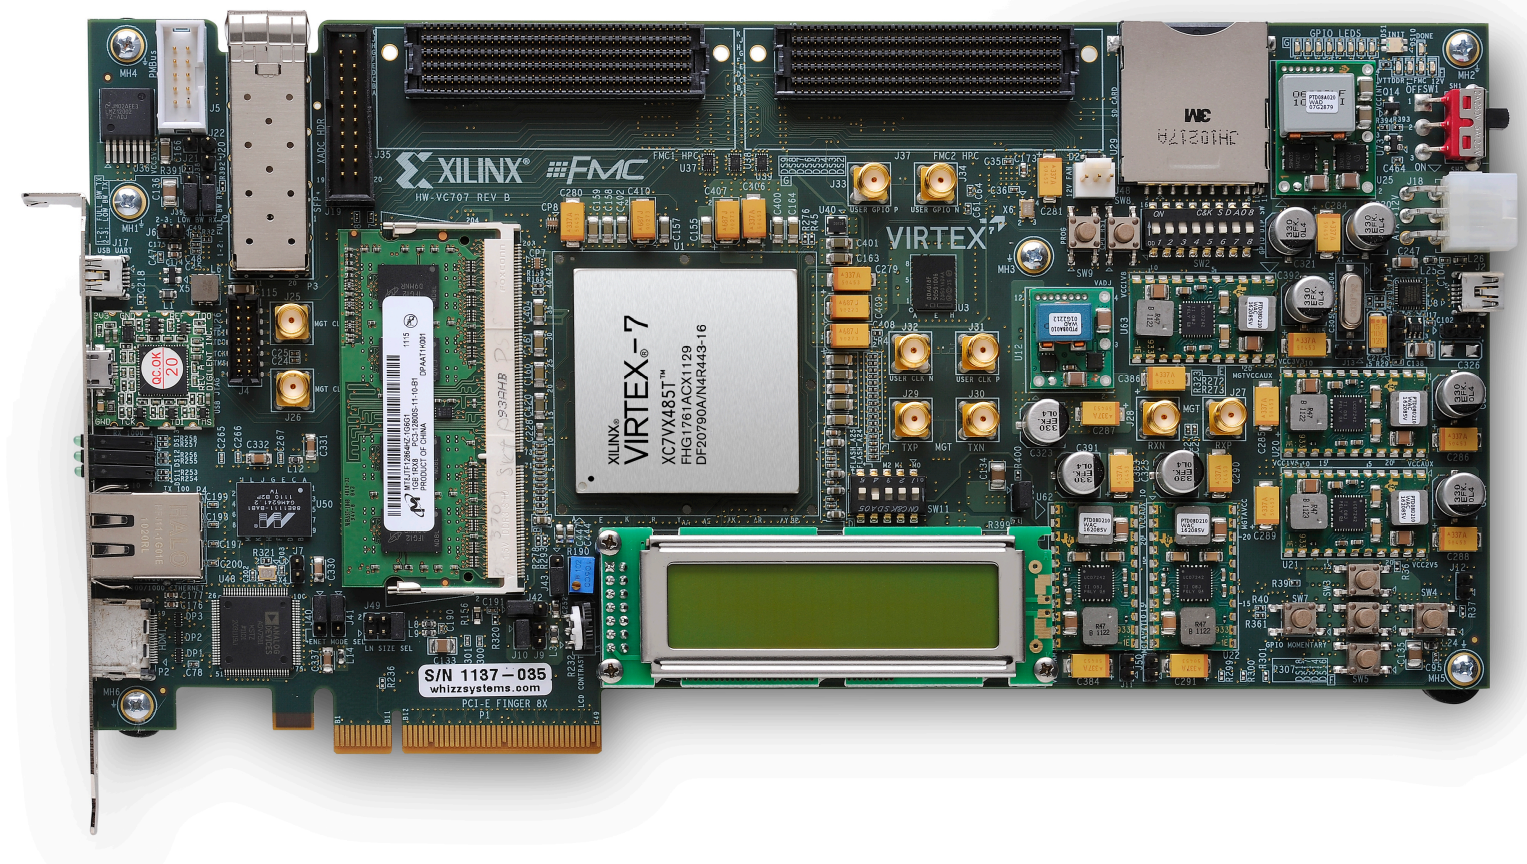
\includegraphics[width=0.4\textwidth]{image/VC707.png}
	\caption{Внешний вид отладочной платы VC707}
	\label{VC707}
\end{figure}

Исходные файлы Verilog описывают только поведение схемы. Вы также должны предоставить файл ограничений, чтобы сопоставить ваш дизайн с физическим чипом и платой, с которыми вы работаете.
В файле ограничений указывается к какому физическому выводу ПЛИС подключечается данный вывод нашего Verilog модуля, а также электрический стандарт используемый для вывода.

Для того чтобы определить, к каким выводам ПЛИС подключать сигналы, недостаточно информации, имеющейся в САПР или в документации на саму ПЛИС. После установки ПЛИС на плату внешние компоненты могут быть подключены производятелем платы самыми разными способами, поэтому требуется обратиться к технической документации на печатную плату. Для проекта была выбрана плата VC707 производства компании Xilinx, на которой и установлена ПЛИС Virtex-7, заданная в настройках проекта. Внешний вид платы представлен на рисунке ~\ref{VC707}. Обратившись к технической документации, можно найти следующую информацию:

\begin{enumerate}
	\item AM39, AN39, AR37, AT37, AR35, AP41, AP42, AU39 - выходы ПЛИС подключенные к светодиодам(\verb|GPIO_LED_0|, \verb|GPIO_LED_1| и т.д (см.рис. ~\ref{LEDS}));
	\item AV30, AY33, BA31, BA32, AW30, AY30, BA30, BB31 - входы ПЛИС подключенные к переключателям платы(\verb|GPIO_DIP_SW_0|, \verb|GPIO_DIP_SW_1| и т.д (см.рис. ~\ref{DIP_SWITCH})).
\end{enumerate}

Также для формата xdc обязательным требованием является явное указание электрического стандарта, используемого для вывода. 

По этому поводу необходимо сделать важное пояснение. ПЛИС не имеют возможности подключать заданные разработчиком напряжения к буферам ввода-вывода, ориентируясь на заданные в файле xdc 
сведения. Для питания будут использованы напряжения, фактически поданные на банки ввода-вывода. Неверное указание напряжения в файле xdc не приведет к выходу ПЛИС из строя, однако рассчи- задержки распространения сигналов окажутся неверными ( они зависят от используемого напряжения питания). Однако для всех выводов, находящихся в одном банке ввода-вывода, требуется, чтобы напряжение электрических интерфейсов было одним и тем. Потому разработчик должен явно указать в файле проектных ограничений электрический интерфейс, который он рассчитывает использовать При появлении в одном банке интерфейсов с разным напряжением САПР сгенерирует ошибку и создание конфигурациного файла будет запрещено. 

Рассмотрим пример:

\begin{Verbatim}[tabsize=4]
set_property PACKAGE_PIN AM39 [get_ports {led[0]}]
set_property IOSTANDARD LVCMOS18 [get_ports {led[0]}]
\end{Verbatim}

Первая строка подключает вывод \verb|led[0]| к контакту AM39 ПЛИС. Вторая строка задаёт  электрический стандарт LVCMOS18 для этого вывода.

Чтобы создать файл ограничений, разверните заголовок «Constraints» на панели «Sources», щелкните правой кнопкой мыши \verb|constrs_1| и выберите «Add Sources» (или, что то же самое, нажмите «Add Sources» в окне «Flow Navigator» в «Project Manager»)(см. рис. ~\ref{add_xdc}, ~\ref{add_xdc_0}) .

Появится диалоговое окно «Add Sources». Выберите «Add or Create Constraints» и нажмите «Далее», чтобы открыть диалоговое окно «Add or Create Constraints».

Нажмите «Create File», введите имя файла «top» и нажмите «ОК». Вновь созданный файл появится в списке, как показано на рисунке. Нажмите Готово, чтобы перейти к следующему шагу.

\begin{Verbatim}[tabsize=4]
# LEDs
set_property PACKAGE_PIN AM39 [get_ports {led[0]}]
set_property IOSTANDARD LVCMOS18 [get_ports {led[0]}]
set_property PACKAGE_PIN AN39 [get_ports {led[1]}]
set_property IOSTANDARD LVCMOS18 [get_ports {led[1]}]
set_property PACKAGE_PIN AR37 [get_ports {led[2]}]
set_property IOSTANDARD LVCMOS18 [get_ports {led[2]}]
set_property PACKAGE_PIN AT37 [get_ports {led[3]}]
set_property IOSTANDARD LVCMOS18 [get_ports {led[3]}]
set_property PACKAGE_PIN AR35 [get_ports {led[4]}]
set_property IOSTANDARD LVCMOS18 [get_ports {led[4]}]
set_property PACKAGE_PIN AP41 [get_ports {led[5]}]
set_property IOSTANDARD LVCMOS18 [get_ports {led[5]}]
set_property PACKAGE_PIN AP42 [get_ports {led[6]}]
set_property IOSTANDARD LVCMOS18 [get_ports {led[6]}]
set_property PACKAGE_PIN AU39 [get_ports {led[7]}]
set_property IOSTANDARD LVCMOS18 [get_ports {led[7]}]

# DIP Switches
set_property PACKAGE_PIN AV30 [get_ports {sw[0]}]
set_property IOSTANDARD LVCMOS18 [get_ports {sw[0]}]
set_property PACKAGE_PIN AY33 [get_ports {sw[1]}]
set_property IOSTANDARD LVCMOS18 [get_ports {sw[1]}]
set_property PACKAGE_PIN BA31 [get_ports {sw[2]}]
set_property IOSTANDARD LVCMOS18 [get_ports {sw[2]}]
set_property PACKAGE_PIN BA32 [get_ports {sw[3]}]
set_property IOSTANDARD LVCMOS18 [get_ports {sw[3]}]
set_property PACKAGE_PIN AW30 [get_ports {sw[4]}]
set_property IOSTANDARD LVCMOS18 [get_ports {sw[4]}]
set_property PACKAGE_PIN AY30 [get_ports {sw[5]}]
set_property IOSTANDARD LVCMOS18 [get_ports {sw[5]}]
set_property PACKAGE_PIN BA30 [get_ports {sw[6]}]
set_property IOSTANDARD LVCMOS18 [get_ports {sw[6]}]
set_property PACKAGE_PIN BB31 [get_ports {sw[7]}]
set_property IOSTANDARD LVCMOS18 [get_ports {sw[7]}]
\end{Verbatim}

Теперь вы увидите файл \verb|top.xdc| в списке под папкой \verb|Constraints/constrs_1| на панели «SourcesИ». Дважды щелкните \verb|top.xdc|, чтобы открыть файл, и замените содержимое приведенным ниже кодом.

\subsubsection{Основы моделирования в Vivado}

Чтобы создать исходный файл моделирования для вашего проекта, щелкните правой кнопкой мыши «Simulation Sources» на панели «Sources» и выберите «Add sources». Появится диалоговое окно «Add sources», как показано - выберите «Add or create simulation sources» и нажмите «Next». На рисунках ниже представлен подробный алгоритм добавления нового файла верификации.

В диалоговом окне «Add or create simulation sources» нажмите «Create File», введите имя файла \verb|tb_sw_led.v| и нажмите «ОК». Вновь созданный файл появится в списке, как показано на рисунке. Нажмите Finish, чтобы перейти к следующему шагу. Теперь вы увидите, что \verb|tb_sw_led.v| указан в папке «Simulation Sources» на панели «Sources». 

Дважды щелкните \verb|tb_sw_led.v|, чтобы открыть файл, и замените содержимое (скопируйте и вставьте) приведенным ниже кодом.

\begin{figure}[htbp]	
	\subfigure[Add or create simulation source] 
	{
		\begin{minipage}{8cm}
			\centering         
			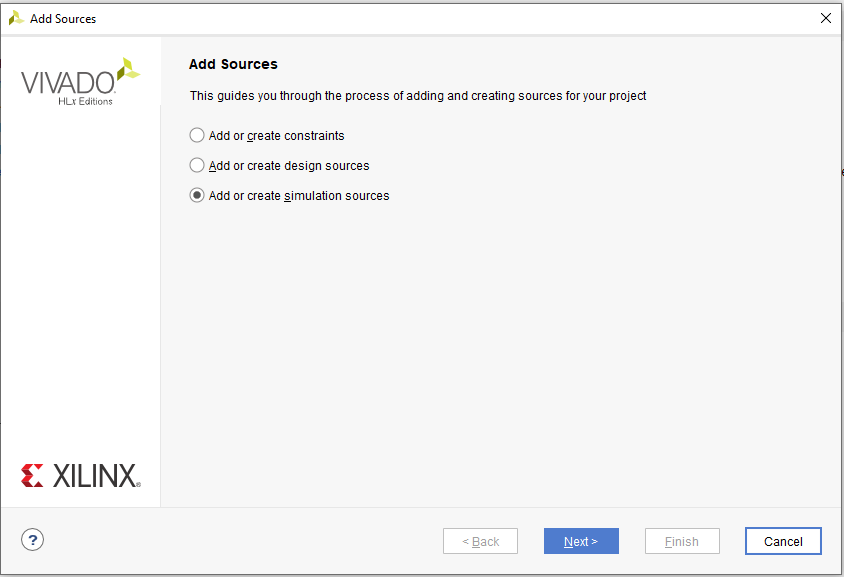
\includegraphics[scale=0.3]{image/l1_sim_1.png}   
			\label{Start_V}
		\end{minipage}
	}
	\subfigure[Окно мастера подключения нового файла] 
	{
		\begin{minipage}{8cm}
			\centering      
			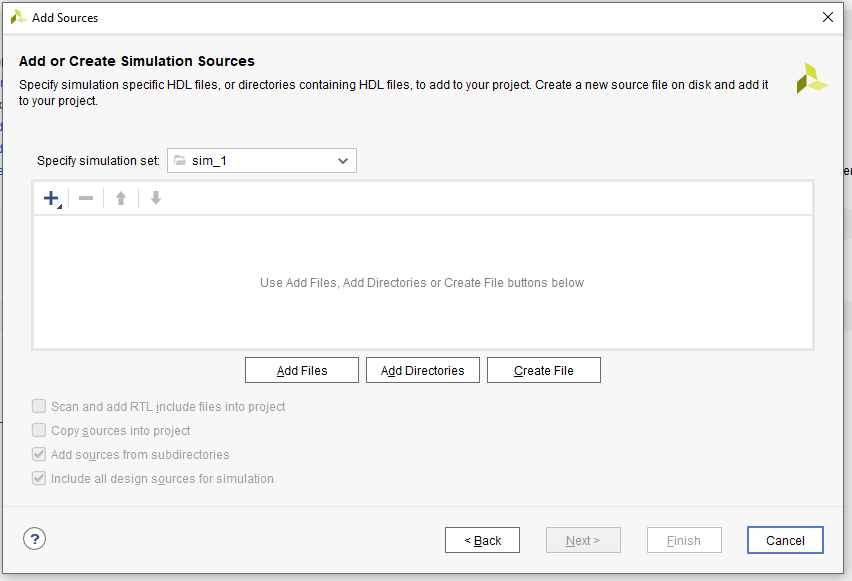
\includegraphics[scale=0.3]{image/l1_sim_2.png}   
			\label{Win_Project}
		\end{minipage}
	}
	\caption{Окно мастера подключения нового файла: внешний вид} %  %Имя большого изображения
\end{figure}

\begin{figure}[htbp]	
	\subfigure[Назначаем файлу моделирования имя] 
	{
		\begin{minipage}{8cm}
			\centering         
			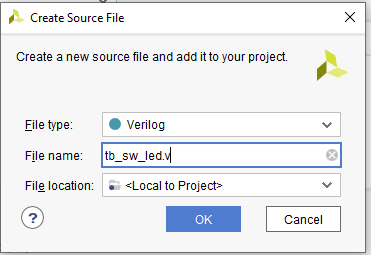
\includegraphics[scale=0.7]{image/l1_sim_3.png}   
			\label{Start_V}
		\end{minipage}
	}
	\subfigure[Результаты добавления файла моделирования] 
	{
		\begin{minipage}{8cm}
			\centering      
			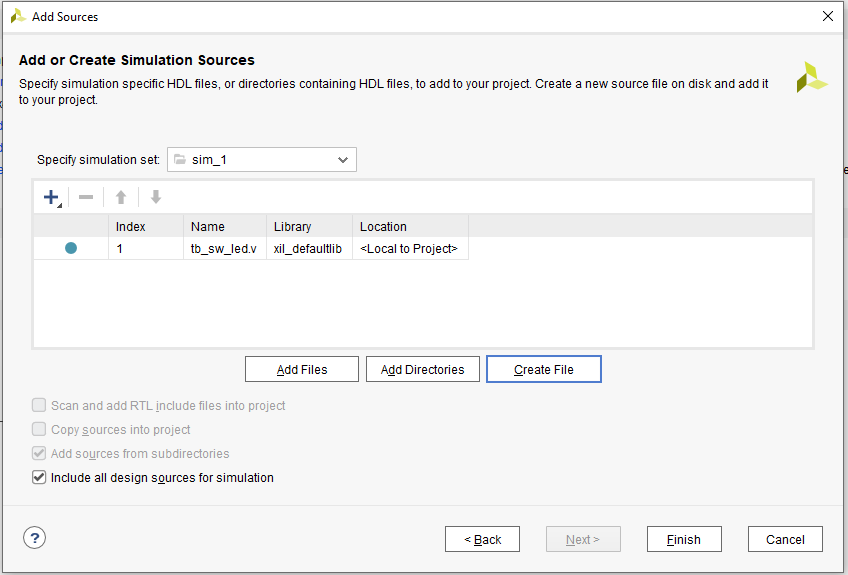
\includegraphics[scale=0.4]{image/l1_sim_4.png}   
			\label{Win_Project}
		\end{minipage}
	}
	\caption{Окно мастера подключения нового файла: имя и результаты} %  %Имя большого изображения
\end{figure}

\begin{Verbatim}[tabsize=4]
`timescale 1ns / 1ps
module tb_sw_led();
    
reg [7:0] sw_led_reg;
wire [7:0] led_w;

sw_led
sw_led_inst
(
    .sw(sw_led_reg),
    .led(led_w)
);

initial begin
    $display("Result:",);
    $timeformat(-9,1,"ns",8);
    $monitor($time, 
    	": 	sw[0] & sw[1]= %b; 
    		sw[2] | sw[3]=%b; 
    		sw[4] ^ sw[5]=%b; 
    		~sw[6]=%b; 
    		sw[7] = %b;", 
    		led_w[0],
    		led_w[1], 
    		led_w[2], 
    		led_w[3], 
    		led_w[4]);
    sw_led_reg[0] = 0;
    sw_led_reg[1] = 0;
    sw_led_reg[2] = 0;
    sw_led_reg[3] = 0;
    sw_led_reg[4] = 0;
    sw_led_reg[5] = 0;
    sw_led_reg[6] = 0;
    sw_led_reg[7] = 0;
    #100;
    sw_led_reg[0] = 0;
    sw_led_reg[1] = 1;
    sw_led_reg[2] = 0;
    sw_led_reg[3] = 1;
    sw_led_reg[4] = 0;
    sw_led_reg[5] = 1;
    sw_led_reg[6] = 0;
    sw_led_reg[7] = 1;
    #100;
    sw_led_reg[0] = 1;
    sw_led_reg[1] = 0;
    sw_led_reg[2] = 1;
    sw_led_reg[3] = 0;
    sw_led_reg[4] = 1;
    sw_led_reg[5] = 0;
    sw_led_reg[6] = 1;
    sw_led_reg[7] = 0;
    #100;
    sw_led_reg[0] = 1;
    sw_led_reg[1] = 1;
    sw_led_reg[2] = 1;
    sw_led_reg[3] = 1;
    sw_led_reg[4] = 1;
    sw_led_reg[5] = 1;
    sw_led_reg[6] = 1;
    sw_led_reg[7] = 1;
end

endmodule
\end{Verbatim}

\begin{figure}[!ht]
	\centering
	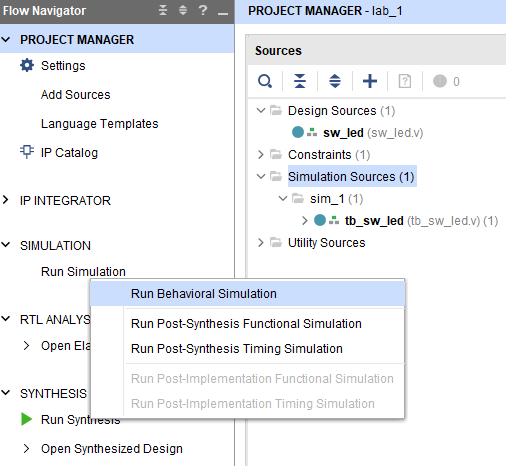
\includegraphics[width=0.4\textwidth]{image/sim_rub.png}
	\caption{Запуск симуляции в среде Vivado}
	\label{prj_sum}
\end{figure}

\begin{figure}[!ht]
	\centering
	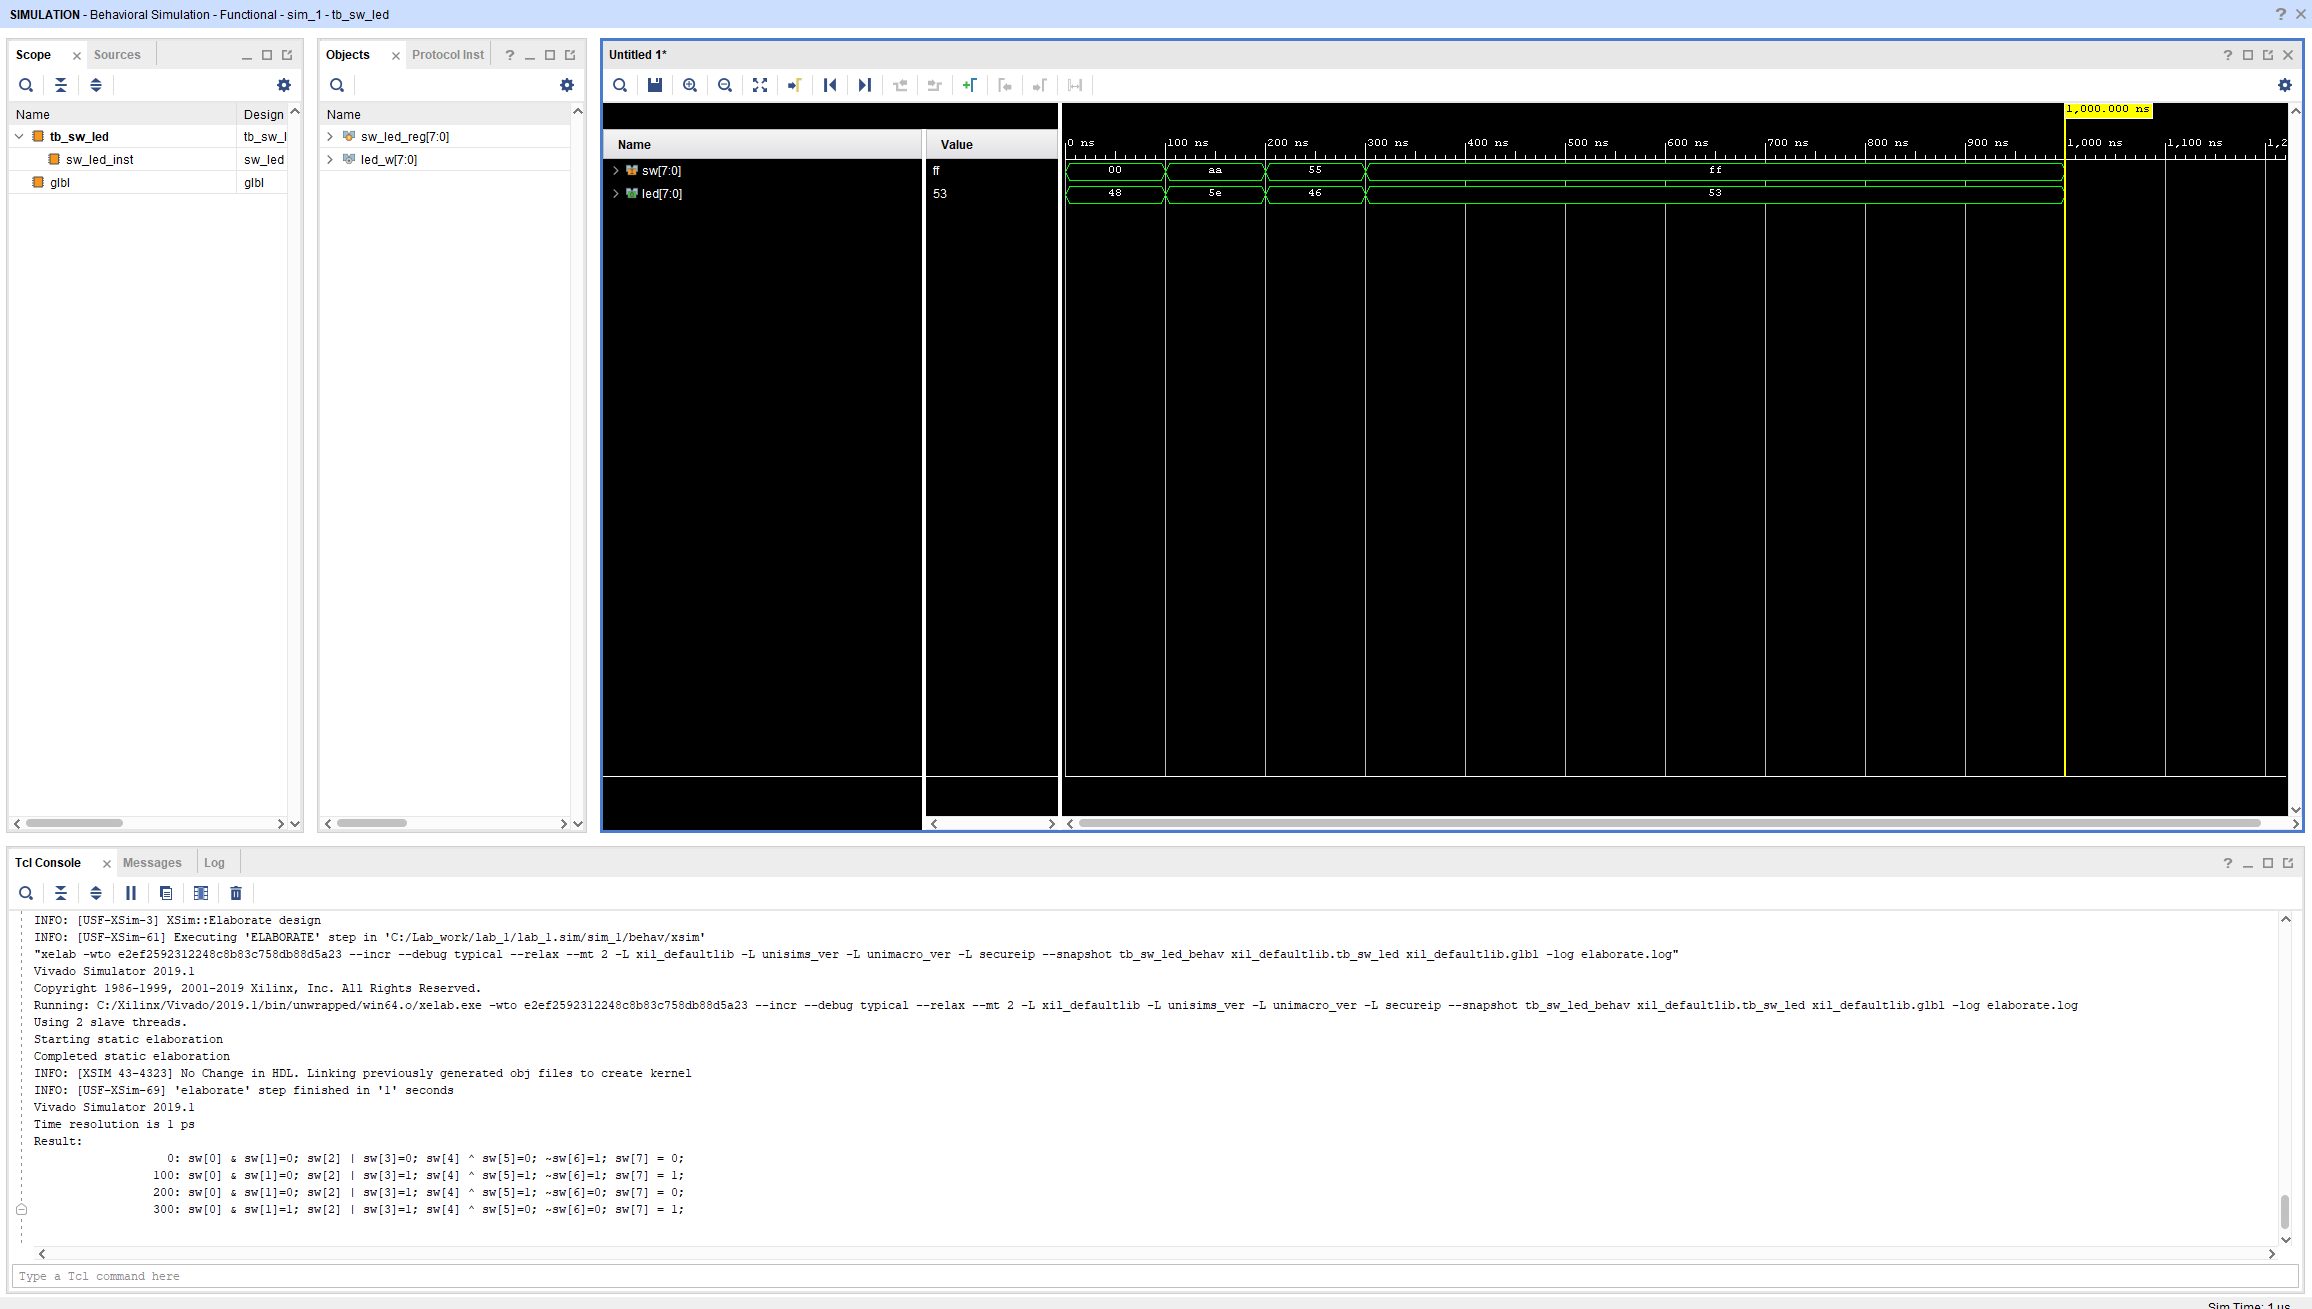
\includegraphics[width=0.7\textwidth]{image/l1_sim_5.png}
	\caption{Окно симуляции в среде Vivado}
	\label{prj_sum}
\end{figure}

Для запуска моделирования нажмите Run Simulation на панели Flow Navigator.
Результат симуляции схемы.

\begin{Verbatim}[tabsize=4]
Result: 

0: sw[0] & sw[1]=0; sw[2] | sw[3]=0; sw[4] ^ sw[5]=0;~sw[6]=1;sw[7] = 0;
100: sw[0] & sw[1]=0; sw[2] | sw[3]=1; sw[4] ^ sw[5]=1;~sw[6]=1;sw[7] = 1;
200: sw[0] & sw[1]=0; sw[2] | sw[3]=1; sw[4] ^ sw[5]=1;~sw[6]=0;sw[7] = 0;
300: sw[0] & sw[1]=1; sw[2] | sw[3]=1; sw[4] ^ sw[5]=0;~sw[6]=0;sw[7] = 1;
\end{Verbatim}
\subsection{Шаг 3: Synthesis, Implementation, and Generate Bitstream}

\subsubsection{Синтез}

После того, как ваши файлы Verilog и файлы ограничений будут завершены, вы можете синтезировать проект. В процессе синтеза код Verilog преобразуется в «список соединений», который определяет все необходимые компоненты схемы(эти компоненты являются программируемыми частями целевого логического устройства). Вы можете запустить процесс синтеза, нажав кнопку «Run Synthesis» на панели «Flow Navigator», как показано на рисунке.

Примечание. В конце процесса синтеза открывается диалоговое окно с вопросом, что вы хотите делать дальше. Это просто удобство — он показывает те же варианты, что и в окне Flow Navigator. Вы можете просто закрыть окно или выбрать «Implement Design», который является следующим шагом (см. ниже).

\begin{figure}[!ht]
	\centering
	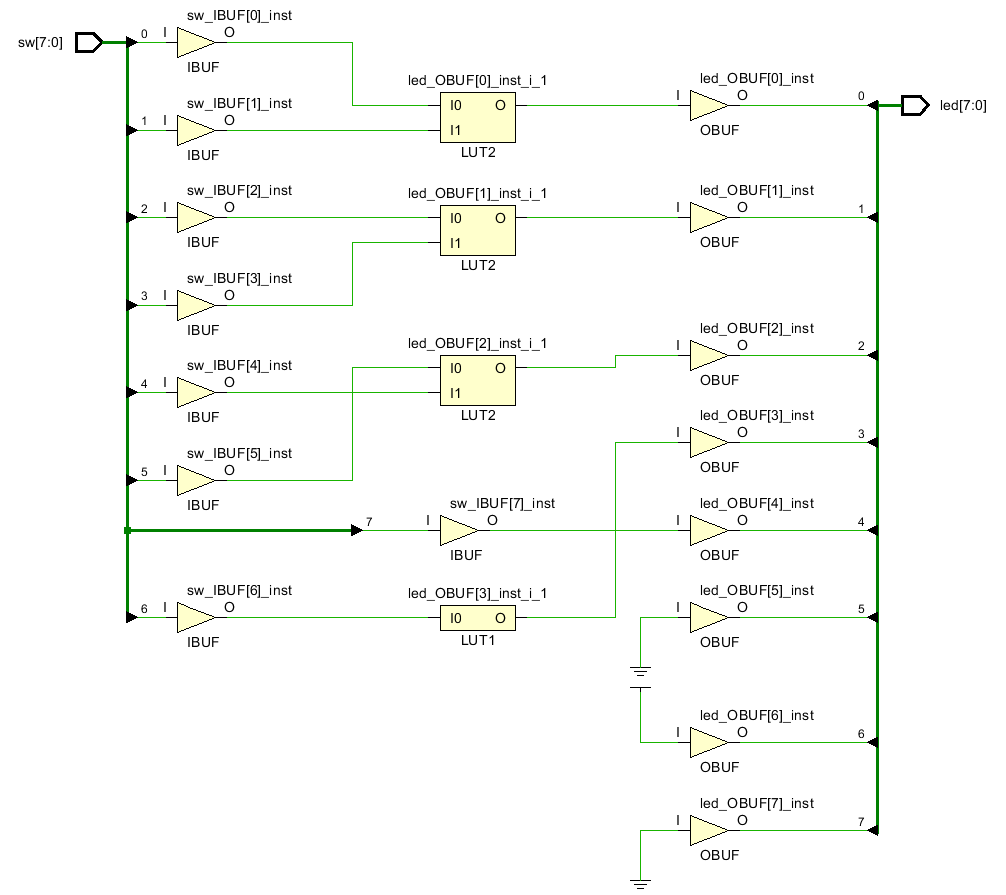
\includegraphics[width=0.7\textwidth]{image/synth.PNG}
	\caption{Синтезированный дизайн}
	\label{l1_synth}
\end{figure}

\subsubsection{Размещение и трассировка проекта}

Эта группа проектных действий входит в состав стадии САПР implementation, название которой дословно можно перевести как «реализация» или сосуществление», однако в русском языке этот термин является не сколько неопределенным и его трудно однозначно связать с проектным шагом, а не просто с общим процессом работы над проектом. 
На данной стадии производится преобразование списка связей в информацию о размещении отдельных элементов ПЛИС на кристалле и настройке программируемых соединений между ними. 
Сведения о структуре ПЛИС и формате конфигурационной последовательности являются закрытыми, и этот шаг может быть реализован только с помощью САПР Xilinx.

Нажмите кнопку «Run Implementation» на панели Flow Navigator, как показано на рисунке.

Примечание. В конце этого процесса открывается диалоговое окно с вопросом, что вы хотите делать дальше. Это просто удобство — он показывает те же варианты, что и в окне Flow Navigator. Вы можете просто закрыть окно или выбрать «Generate Bitstream», который является следующим шагом (см. ниже).

\subsubsection{Генерация .bit файла}
После успешной завершения процесса размещения и трассировка проекта вы можете создать файл .bit, щелкнув процесс Generate Bitstream, расположенный на панели Flow Navigator, как показано. Процесс переводит реализованный дизайн в битовый поток, который можно напрямую запрограммировать на устройстве вашей платы.

Примечание. В конце процесса генерации .bit файла открывается диалоговое окно с вопросом, что вы хотите делать дальше. Это просто удобство — он показывает те же варианты, что и в окне Flow Navigator. Вы можете просто закрыть окно или выбрать «Open Hardware Manager», что является следующим шагом (см. ниже).

\subsection{Шаг 4: Загрузка конфигурационного файла в ПЛИС}

После того, как bitstream будет успешно сгенерирован, вы можете запрограммировать плату с помощью Hardware Manager. Щелкните Open Hardware Manager, расположенный в нижней части панели Flow Navigator, как показано красным на рисунке. Следуйте указаниям на рисунках ~\ref{l1_hard_1}, ~\ref{l1_hard_2}, ~\ref{l1_hard_3},~\ref{l1_hard_4}, 
 ~\ref{l1_hard_5},~\ref{l1_hard_6}, ~\ref{l1_hard_7} чтобы прошить ПЛИС.

\begin{figure}[htbp]	
	\subfigure[Open New Target] 
	{
		\begin{minipage}{8cm}
			\centering         
			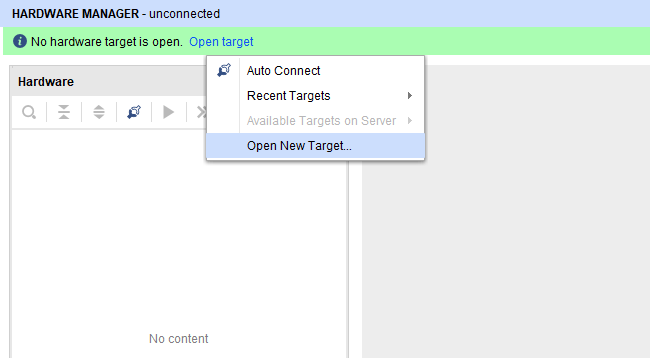
\includegraphics[scale=0.4]{image/l1_hard_1.png}   
			\label{l1_hard_1}
		\end{minipage}
	}
	\subfigure[Окно мастера подключения нового устройства] 
	{
		\begin{minipage}{8cm}
			\centering      
			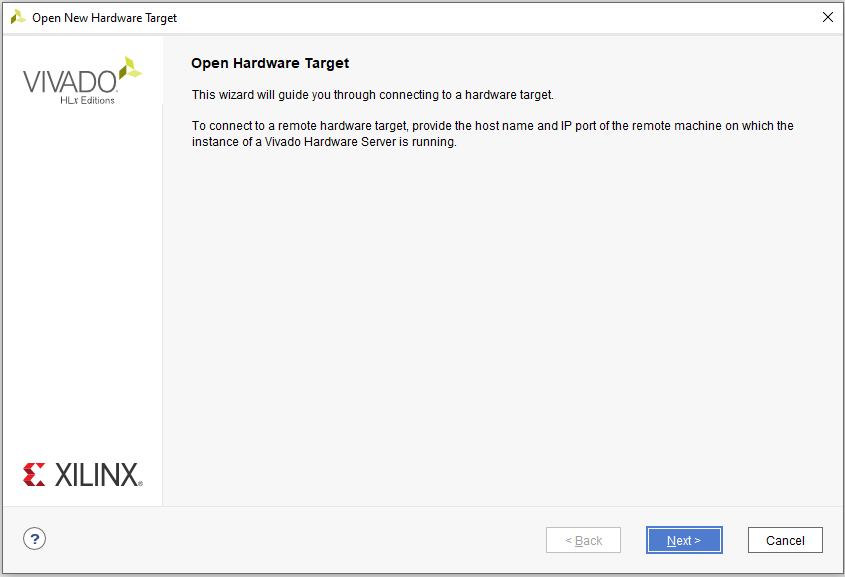
\includegraphics[scale=0.4]{image/l1_hard_2.png}   
			\label{l1_hard_2}
		\end{minipage}
	}
	\caption{Окно мастера подключения нового устройства: внешний вид} %  %Имя большого изображения
\end{figure}

\begin{figure}[htbp]	
	\subfigure[Hardware Server Setting] 
	{
		\begin{minipage}{9cm}
			\centering         
			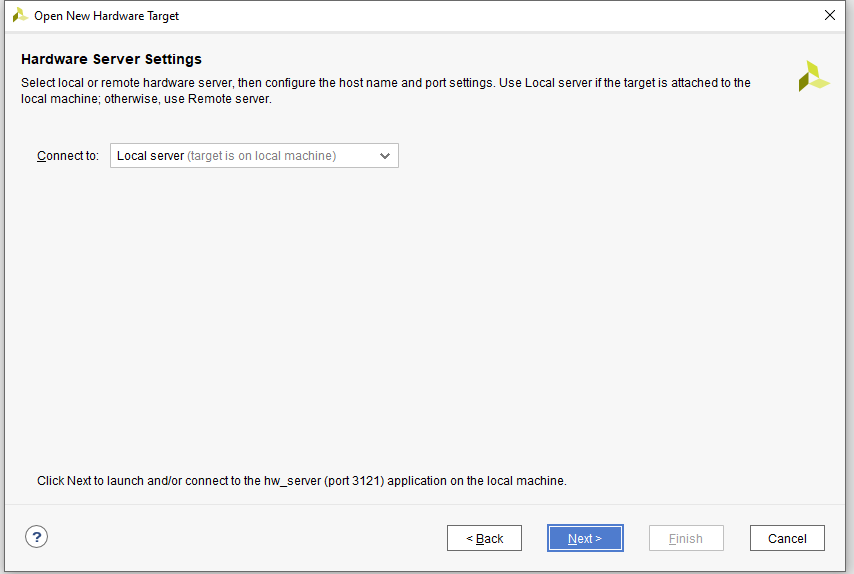
\includegraphics[scale=0.4]{image/l1_hard_3.png} 
			\label{l1_hard_3}
		\end{minipage}
	}
	\subfigure[Select Hardware Target] 
	{
		\begin{minipage}{9cm}
			\centering      
			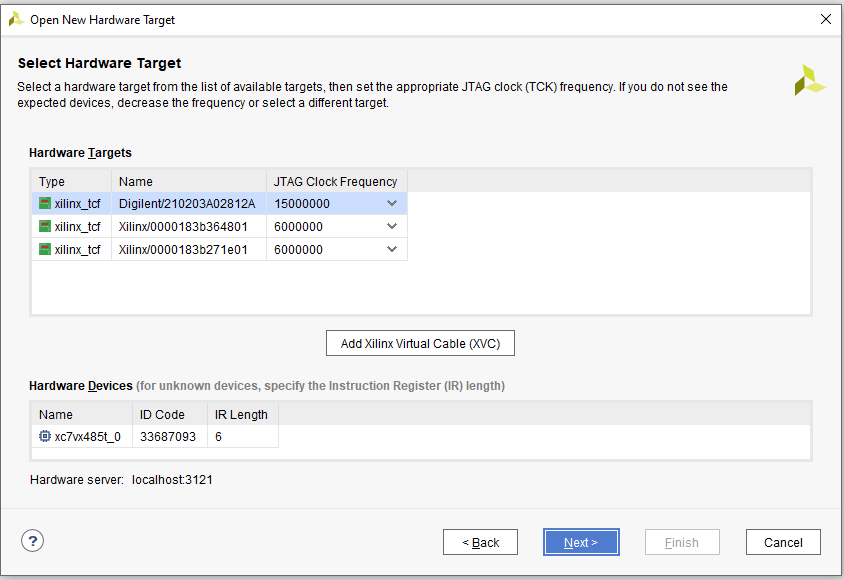
\includegraphics[scale=0.4]{image/l1_hard_4.png} 
			\label{l1_hard_4}
		\end{minipage}
	}
	\caption{Окно мастера подключения нового устройства: выбор устройства} %  %Имя большого изображения
\end{figure}

\begin{figure}[!ht]
	\centering
	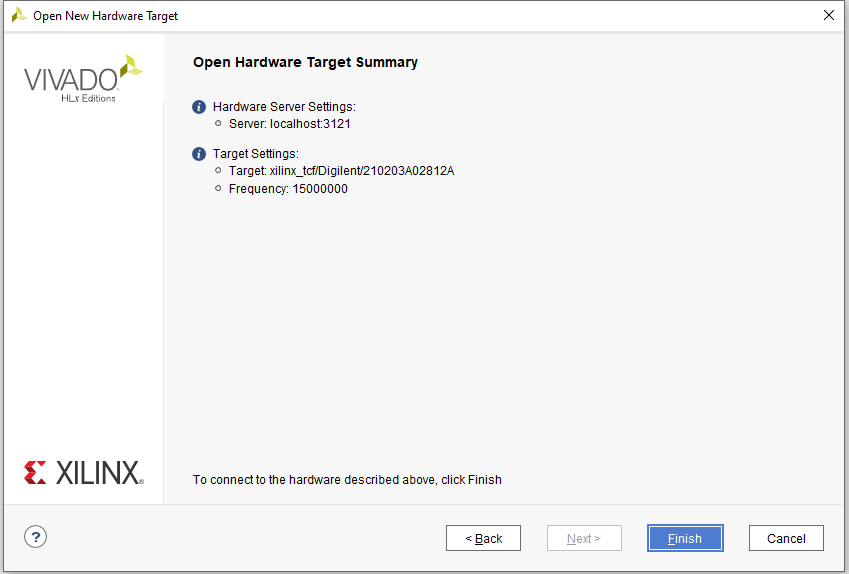
\includegraphics[width=0.5\textwidth]{image/l1_hard_sum.png}
	\caption{Окно мастера подключения нового устройства: результаты}
	\label{l1_hard_5}
\end{figure}

\begin{figure}[htbp]	
	\subfigure[Результаты подключения нового устройства] 
	{
		\begin{minipage}{8cm}
			\centering         
			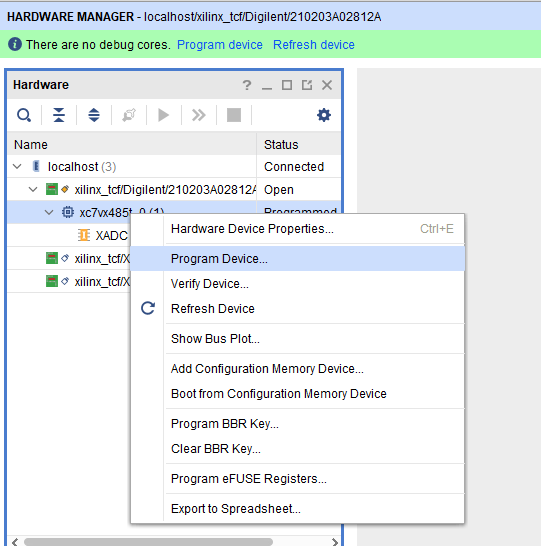
\includegraphics[scale=0.4]{image/program_0.png} 
			\label{l1_hard_6}
		\end{minipage}
	}
	\subfigure[Указываем путь к прошивке] 
	{
		\begin{minipage}{8cm}
			\centering      
			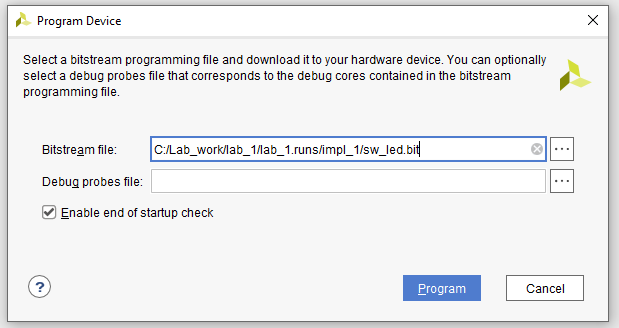
\includegraphics[scale=0.6]{image/program.png} 
			\label{l1_hard_7}
		\end{minipage}
	}
	\caption{Программирование ПЛИС} %  %Имя большого изображения
\end{figure}

\section{Иерархия проекта и простые логические элементы}

В проекте, особенно сложном, бывает много модулей, соединенных между собой. Прежде
всего, нужно заметить, что обычно в проекте всегда есть один модуль самого верхнего уровня
(top level). Внутри тела модуля верхнего уровня объявляються экземпляры других модулей и потом
соединяються друг с другом проводами. Рассмотрим как это делается на простейшом примере.

Логические модули И и И-НЕ можно описать на языке Verilog следующим образом: 

\begin{Verbatim}[tabsize=4]
module AND(output OUT, input IN1, input IN2);
 	assign OUT = IN1 & IN2;
endmodule
module NAND(output OUT, input IN1, input IN2);
 	assign OUT = ~(IN1 & IN2);
endmodule
\end{Verbatim}

Логические модули ИЛИ и ИЛИ-НЕ можно описать на языке Verilog следующим образом: 

\begin{Verbatim}[tabsize=4]
module OR(output OUT, input IN1, input IN2);
 	assign OUT = IN1 | IN2;
endmodule
module NOR(output OUT, input IN1, input IN2);
 	assign OUT = ~(IN1 | IN2);
endmodule
\end{Verbatim}

Логические модули Исключающее ИЛИ и Исключающее ИЛИ-НЕ, а также элемент НЕ 
можно описать на языке Verilog следующим образом: 

\begin{Verbatim}[tabsize=4]
module XOR(output OUT, input IN1, input IN2);
 	assign OUT = IN1 ^ IN2;
endmodule
module XNOR(output OUT, input IN1, input IN2);
 	assign OUT = ~(IN1 ^ IN2);
endmodule
module INV(output OUT, input IN);
 	assign OUT = ~IN;
endmodule
\end{Verbatim}

Итак, мы знаем про основные базовые логические элементы – и это тоже модули. Используем
их в модуле более высокого уровня. Сделаем однобитный сумматор по вот такой схеме: 

\begin{figure}[!ht]
	\centering
	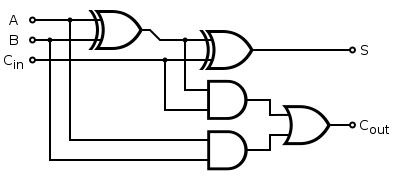
\includegraphics[width=0.7\textwidth]{image/Full_Adder.PNG}
	\caption{Полный сумматор на логических элементах}
	\label{full_adder}
\end{figure}

Этот сумматор складывает два однобитных числа a и b. При выполнении сложения однобитных
чисел может случиться «переполнение», то есть результат уже будет двухбитным (1+1=2 или в
двоичном виде 1’b1+1’b1=2’b10). Поэтому у нас есть выходной сигнал переноса \verb|c_out|.
Дополнительный входной сигнал \verb|c_in| служит для приема сигнала переноса от сумматоров
младших разрядов, при построении многобитных сумматоров.
Посмотрите, как можно описать эту схему на языке Verilog, устанавливая в теле модуля
экземпляры других модулей.

\begin{Verbatim}[tabsize=4]
module adder1 (
	output wire sum, 
	output wire c_out, 
	input wire a, 
	input wire b, 
	input wire c_in
); 
wire s1,s2,s3; 
AND and_inst_1
( 
	.OUT (s1), 
	.IN1 (a), 
	.IN2 (b) 
); 
XOR xor_inst_1
( 
	.OUT (s2), 
	.IN1 (a), 
	.IN2 (b) 
);
AND and_inst_2
( 
	.OUT (s3), 
	.IN1 (s2), 
	.IN2 (c_in) 
); 
OR or_inst
( 
	.OUT (c_out), 
	.IN1 (s1), 
	.IN2 (s3) 
); 
XOR xor_inst_3
(
	.OUT (c_out), 
	.IN1 (s2), 
	.IN2 (c_in)
);
endmodule
\end{Verbatim}

Порядок описания экземпляра модуля такой:

\begin{itemize}
    \item Пишем название модуля, тип которого нам нужен.
    \item Пишем название конкретно этого экземпляра модуля по шаблону  \verb|имя_inst|.
    \item Описываем подключения сигналов: точка и затем имя сигнала модуля, затем в скобках
имя проводника, который сюда подключен. 

\end{itemize}
 
Конечно, совсем не обязательо описывать наш модуль так, как описано выше. Честно говоря,
мне гораздо приятней видеть вот такой код однобитного сумматора: 

\begin{Verbatim}[tabsize=4]
module adder1(
	output wire sum, 
	output wire c_out, 
	input wire a, 
	input wire b, 
	input wire c_in
);
	assign sum = (a^b) ^ c_in;
	assign c_out = (a & b) |  (c_in & (a ^ b));
endmodule
\end{Verbatim}

Просто важно понимать, что существуют разные методы описания, и нужно уметь ими всеми
пользоваться.

\section{Мультиплексор и параметризация модуля}

Рассмотрим реализацию мультиплексора 2->1 на языке Verilog.

\begin{Verbatim}[tabsize=4]
module mux_2to1 ( 
	input wire a,                   
	input wire b,                                    
	input sel,               
	output out
);             
  
   assign out = sel ? b : a;  
  
endmodule  
\end{Verbatim}

Усложним задачу и построим мультиплексор 4->1. 

\begin{Verbatim}[tabsize=4]
module mux_4to1 ( 
	input wire a,                   
	input wire b,                   
	input wire c,                   
	input wire d,                   
	input [1:0] sel,               
	output out
);             
  
   assign out = sel[1] ? (sel[0] ? d : c) : (sel[0] ? b : a);  
  
endmodule  
\end{Verbatim}

Пусть теперь мы хотим коммутировать не просто провода, а шины, при этом нам нужно два мультиплексора под различные размеры шин. Пусть один мультиплексор коммутирует 8-битные шины, а другой 16-битные.
Тогда мы получим следующий код:

\begin{Verbatim}[tabsize=4]
module mux_4to1 ( 
	input wire [7:0] a,                   
	input wire [7:0] b,                   
	input wire [7:0] c,                   
	input wire [7:0] d,                   
	input [1:0] sel,               
	output [7:0] out
);             
  
   assign out = sel[1] ? (sel[0] ? d : c) : (sel[0] ? b : a);  
  
endmodule  
\end{Verbatim}

\begin{Verbatim}[tabsize=4]
module mux_4to1 ( 
	input wire [15:0] a,                   
	input wire [15:0] b,                   
	input wire [15:0] c,                   
	input wire [15:0] d,                   
	input [1:0] sel,               
	output [15:0] out
);             
  
   assign out = sel[1] ? (sel[0] ? d : c) : (sel[0] ? b : a);  
  
endmodule  
\end{Verbatim}

Эти модули не отличаются ни чем, кроме размера шин.
Используя параметризацию в языке Verilog можно построить мультиплексор с размером шины переменным(до синтеза), а не постоянным. Параметризованный модуль мультиплексора имеет следующий вид:

\begin{Verbatim}[tabsize=4]
module mux_4to1 #(
	parameter DATA_WIDTH = 8
) 
( 
	input wire [DATA_WIDTH - 1:0] a,                   
	input wire [DATA_WIDTH - 1:0] b,                   
	input wire [DATA_WIDTH - 1:0] c,                   
	input wire [DATA_WIDTH - 1:0] d,                   
	input [1:0] sel,               
	output [DATA_WIDTH - 1:0] out
);             
  
   assign out = sel[1] ? (sel[0] ? d : c) : (sel[0] ? b : a);  
  
endmodule  
\end{Verbatim}

При этом для подключения такого модуля используется следующий синтаксис:

\begin{Verbatim}[tabsize=4]
mux_4to1 #(
	.DATA_WIDTH(8)
)
mux_4to1_inst
( 
	.a(),                   
	.b(),                   
	.c(),                   
	.d(),                   
	.sel(),               
	.out()
);             
\end{Verbatim}

\newpage

Вопросы: 
\begin{enumerate}
\item Проведите функциональную симуляцию схемы по заданным входным сигналам a, b, clk.
\item 
\item 
\end{enumerate}

Задания:

\begin{enumerate}
	\item Реализовать модуль сумматора, используя простейшие логические элементы как отдельные модули, то есть необходимо получить проект с иерархией(см. подпункт. 1.2).
	\item Реализовать на языке Verilog следующие модули(число N узнать у преподавателя):
	\begin{enumerate}
		\item Шифратор (двоичный). На входе: \(2^N\)-битная маска вида 0010 (\verb|data_i|).
		На выходе: N-битное число, которое показывает номер бита, в котором выставлена единица (\verb|num_o|).
		
		\item Дешифратор (двоичный). На входе: N-битное число (\verb|num_i|). На выходе: \(2^N\) двоичная маска (\verb|dec_o|), 
		где стоит единица в бите под тем номером, который подан на вход.
		
		\item Мультиплексор. На входе: \(2^N\)-битные данные (\verb|data_i|), N-битный номер для выбора (\verb|num_i|).
		На выходе: значение бита, которой расположен под номером \verb|num_i|.

		\item Демультиплексор. На входе: один бит данных (\verb|data_i|), N-битный номер (\verb|num_i|).
		На выходе: данные размером \(2^N\) (\verb|data_o|), в бите под номером \verb|num_i| должно быть выставлено значение \verb|data_i|. Во всех остальных битах - нули.
	\end{enumerate}
	\item Реализовать на языке Verilog следующие логические функции:
	\begin{enumerate}
		\item (a XOR b) OR (c AND d)) AND (a AND b) OR (NOT c). 
		\item ((a OR d) AND (NOT c)) OR (d AND a) OR (c OR d) .
		\item (a AND b AND c ) OR ((c AND d) AND (c OR a)) OR (NOT d).
		\item (d XOR c) OR ((d XOR a) AND (c OR b)) AND (NOT a).
	\end{enumerate}
\end{enumerate}

\textbf{Для каждого представленного выше задания необходимо}:
\begin{enumerate}
\item Написать синтезируемый модуль, который решает поставленную задачу.
\item Написать модуль-тестбенч (testbench) к этому модулю.
\item Сделать проект в Vivado. Собрать модуль согласно заданию. 
\item Провести симуляцию в Vivado. Убедиться, что модуль корректно работает.
\item Написать файл ограничений для каждого проекта. Входы подключаем к кнопках, выходы к светодиодам.
\item Убедится, что модуль синтезируется, и не возникает латчей, комбинационных петель и пр.. Провести размещение и трассировку проекта, убедиться что нет ошибок. 
\item Сгенерировать конфигурационный файл, убедиться что успешно.
\end{enumerate}

\chapter{Лабораторная работа №2. Реализация ШИМ-контроллера скорости вентилятора}

ШИМ или PWM (широтно-импульсная модуляция, по-английски pulse-width modulation) – это
способ управления подачей мощности к нагрузке. Управление заключается в изменении
длительности импульса при постоянной частоте следования импульсов, то есть при использовании метода широтно-импульсной модуляции, 
частота сигнала и амплитуда остаются постоянными. 
Самым важным параметром сигнала ШИМ является коэффициент заполнения, 
который можно определить по следующей формуле:

\begin{equation}	
	D =  \tau/T
\end{equation}

где \(T\)— период импульсов, \(\tau\)  — длительность импульса, \(D\) — коэффициент заполнения. На рисунках ~\ref{fig:pwm_30}, ~\ref{fig:pwm_70}, ~\ref{fig:pwm_90} представлен ШИМ-сигнал
с различными коэффициентами заполнения.

\begin{figure}[h]
    \centering
    \noindent
    \begin{tikzpicture}
        \begin{axis}
            [
            RCS Plot,
            title={},
            height=0.3\textwidth,
            xlabel={Время, мкс},
            ylabel={Амплитуда, В},
            legend pos = south east
            ]
            \addplot table {Synopsis/data/third-party/pwm_30.dat};
            \addlegendentry{D = 30};
        \end{axis}
    \end{tikzpicture}
    \caption{ШИМ-сигнал с коэффициентом заполнения D = 30}
    \label{fig:pwm_30}
\end{figure}

\begin{figure}[h]
    \centering
    \noindent
    \begin{tikzpicture}
        \begin{axis}
            [
            RCS Plot,
            title={},
            height=0.3\textwidth,
            xlabel={Время, мкс},
            ylabel={Амплитуда, В},
            legend pos = south east
            ]
            \addplot table {Synopsis/data/third-party/pwm_70.dat};
            \addlegendentry{D = 70};
        \end{axis}
    \end{tikzpicture}
    \caption{ШИМ-сигнал с коэффициентом заполнения D = 70}
    \label{fig:pwm_70}
\end{figure}

\begin{figure}[h]
    \centering
    \noindent
    \begin{tikzpicture}
        \begin{axis}
            [
            RCS Plot,
            title={},
            height=0.3\textwidth,
            xlabel={Время, мкс},
            ylabel={Амплитуда, В},
            legend pos = south east
            ]
            \addplot table {Synopsis/data/third-party/pwm_90.dat};
            \addlegendentry{D = 90};
        \end{axis}
    \end{tikzpicture}
    \caption{ШИМ-сигнал с коэффициентом заполнения D = 90}
    \label{fig:pwm_90}
\end{figure}

В качестве коммутационных элементов применяются биполярные и полевые транзисторы,
работающие в ключевом режиме. То есть, часть периода транзистор полностью открыт, 
а часть периода — полностью закрыт. При этом в замкнутом состоянии 
сопротивление транзистора как ключа очень невелико, и падение на нем напряжения приближается к нулю.

После рассмотрения принципов широтно-импульсной модуляции передём к разработке модуля, реализующего данную функцию.
Прежде всего создадим модуль верхнего уровня и рассмотрим вопрос о изменении входной тактовой частоты сигнала равной 200 МГц. .
Для понижение тактовой частоты до 25 МГц используем примитив MMCM(Mixed-Mode Clock Manager). Данный примтив позволяет генерировать до семи различных частот, с различными коэффициентоми заполнения, с различными фазами. Также он может работать в режиме фильтра дрожжания тактового сигнала.
Рассмотрим подробнее параметризацию и принцип работы примитива MMCM, опираясь на документ 7 Series FPGAs Clocking Resources User Guide (UG472). Структурная схема примитива представлена на рисунке ~\ref{MMCM2_BASE}. 

На структурной схемы представлены:

\begin{enumerate}
	\item D - делитель входной частоты;
	\item PFD(phase-frequency detector) - фазовый детектор;
	\item CP(charge pump) - cхемы подкачки заряд;
	\item LF(loop filter) - фильтр нижний частот;
	\item VCO(voltage-controlled oscillator) - генератор управляемый напряжением;
	\item O0,O1,O2,O3,O4,O5,O6 - делители выходных частоты;
	\item M - делитель частоты в петле обратной связи.
\end{enumerate}

На вход MMCM подается две входные тактовые частоты \(F_{CLKIN1}\) и \(F_{CLKIN2}\). Через мультиплексор одна из входных частот поступает на делитель частоты D, где опорная частота делится  и получается другая частота \(F_{PFD}\), 
которая поступает на фазовый детектор PFD (phase-frequency detector).
Фазовый детектор сравнивает фазы частот \(F_{PFD}\) и той, что поступает с делителя M. Разность фаз, фильтруется и подаётся на генератор управляемы напряжением - VCO(voltage-controlled oscillator). Обозначим частоту на выходе генератора управляемого напряжением как \(F_{VCO}\). Фазовый детектор подает управляющее воздействие на генератор VCO до тех пор, пока не выполнится условие \(F_{PFD}\) = \(F_{VCO}\) / M. При этом условии частоты подаваемые на PFD равны. Подбирая коэффициенты D, M можно синтезировать довольно большой диапазон частот. 

\begin{figure}[!ht]
	\centering
	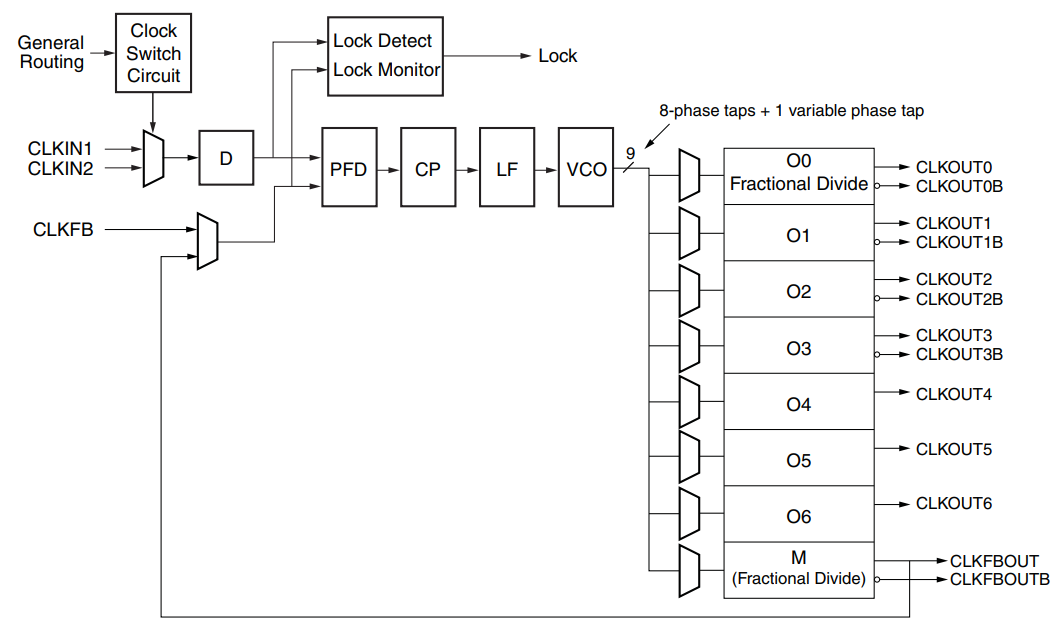
\includegraphics[width=0.5\textwidth]{image/MMCM2_BASE.PNG}
	\caption{Структурная схема примитива MMCM}
	\label{MMCM2_BASE}
\end{figure}

Для того чтобы настроить примитив MMCM необходима следующая информация:

\begin{enumerate}
	\item Частота входного сигнала;
	\item Частоты выходных сигналов(максимум 7);
	\item Коэффициент заполнения выходного сигнала(по умолчанию 50%);
	\item Сдвиг фазы выходных сигналов в градусах относительно фазы входного тактового сигнала;
	\item Полоса пропускания MMCM(по умолчанию установлено значение "OPTIMIZED"), применяется в режиме уменьшения дрожжания("jitter") входного тактового сигнала;
	\item Джиттер("jitter") входного тактового сигнала.
\end{enumerate}

Каждый пункт из списка выше задаётся в виде параметров, назначение, тип данных и диапазон приминимаемых значений которых представлен ниже:

\begin{enumerate}
	\item \verb|BANDWIDTH| определяет алгоритм программирования MMCM, влияющий на джиттер и другие характеристики MMCM. Имеет строковый тип данных и ринимает значения HIGH, LOW, OPTIMIZED.		
	\item \verb|CLKOUT[1:6]_DIVIDE|	 
	определяет величину выходного делителя(обозначен буквой O на структурной схеме) 
	тактовой частоты сигналов CLKOUT[1], CLKOUT[2], CLKOUT[3], CLKOUT[4], CLKOUT[5], CLKOUT[6]. 
	Целое число в диапазоне значений от 1 до 128.
	\item \verb|CLKOUT[0]_DIVIDE_F| определяет величину выходного делителя(обзначен буквой O на структурной схеме) тактовой частоты сигналов CLKOUT[0]. Действительное число в диапазоне значений от 2,000 до 128,000 с шагом 0,125. 	
	\item \verb|CLKOUT[0:6]_PHASE| определяет начальную фазу соответствующего выхода тактового сигнала CLKOUT в смещении в градусах(то есть 90 указывает на сдвиг фазы на 90°). Действительное число в диапазоне от –360.000 до 360.000 in
с шагом 1/56 от FVCO или другим инкрементом, который зависит от \verb|CLKOUT_DIVIDE|.
	\item \verb|CLKOUT[0:6]_DUTY_CYCLE| определяет коэффициент заполнения тактовый сигнала CLKOUT в процентах (то есть 0,50 будет генерировать коэффициент заполнения равный 50\%. Действительное число в диапазоне от 0.01 до 0.99. 
	\item \verb|CLKFBOUT_MULT_F| определяет величину умножения всех выходов тактовых сигналов CLKOUT, если требуется другая частота. Целое число в диапазоне от 2 до 64 или действительное число в диапазоне от 2.000 до 64.000 с инкрементом равным 0.125. 
	\item \verb|DIVCLK_DIVIDE| определяет коэффициент деления для всех выходных тактовых частот по отношению к входной тактовой частоте. Целое число в диапазоне значений от 1 до 106.	
	\item \verb|CLKFBOUT_PHASE| определяет сдвиг фазы в градусах на выходе обратной связи тактового генератора. Сдвиг сигнала обратной связи приводит к отрицательному фазовому сдвигу всех выходных тактовых сигналов на MMCM. Действительное число в диапазоне от 0,00 до 360,00.
	\item \verb|REF_JITTER1| определяет дрожание("jitter") входного тактового сигнала. Действительное число в диапазоне от 0,00 до 0,999.
	Необходим только для моделирования.
	\item \verb|CLKIN1_PERIOD| указывает период входной тактового сигнала в нс для входа MMCM CLKIN1. Разрешение в ps. Эта информация является обязательной и должна быть предоставлена. Действительное число в диапазоне от 0,938 до 100,000. 		
	\item \verb|CLKIN2_PERIOD| указывает период входной тактового сигнала в нс для входа MMCM CLKIN2. Разрешение в ps. Эта информация является обязательной и должна быть предоставлена. Действительное число в диапазоне от 0,938 до 100,000.	
\end{enumerate}

Назначение портов ввода/вывода примитива \(MMCM2_BASE\):

\begin{enumerate}
	\item \verb|CLKIN1(input)| - входной тактовый сигнал №1. 
	\item \verb|CLKIN2(input)| - входной тактовый сигнал №2.
	\item \verb|CLKFBIN(input)| - тактовый сигнал обратной связи.
	\item \verb|CLKINSEL(input)| - управляющий вход мультиплексора выбора входного сигнала: высокий логический уровень \verb|CLKIN1|, 
	низкий логический уровень \verb|CLKIN2|. 
	\item \verb|RST(input)| - асинхронный сигнал сброс.
	\item \verb|PWRDWN(input)| - отключает созданные, но в настоящее время неиспользуемые модули MMCM/PLL. Этот режим можно использовать для экономии энергии для временно неактивных частей схемы и/или MMCM, которые не активны в определенных конфигурациях системы. В этом режиме мощность MMCM/PLL не потребляется. Подайте логическую единицу для отключения MMCM. 
	\item \verb|CLKOUT[0:6](output)| - выходные тактовые сигналы.
	\item \verb|CLKOUT[0:3]B(output)| - инвертированный CLKOUT[0:3].
	\item \verb|CLKFBOUT(output)| - выход обратной связи MMCM.
	\item \verb|CLKFBOUTB(output)| инвертированный выход обратной связи MMCM.
	\item \verb|LOCKED(output)| - выходной сигнал модуля MMCM принимающий значение логической единицы, когда модуль MMCM достиг фазового совмещения в предопределенном окне и согласования частот в предопределенном диапазоне PPM. MMCM автоматически блокируется после включения питания. Дополнительный сброс не требуется. LOCKED принимает значение логического нуля в течение одного тактового цикла частоты фазового детектора, если тактовая частота на входе остановится, будет нарушена синхронизация фаз (например, фазовый сдвиг тактовой частоты на входе) или изменится частота. MMCM должен быть сброшен при снятии подтверждения LOCKED. Тактовые выходы не должны использоваться до утверждения LOCKED.
\end{enumerate}

Рассчитать значение выходной тактовой частоты и значение частоты генератора управляемого напряжением можно по формулам:

\begin{equation}	
	F_{OUT} =  F_{CLKIN} * \frac{M}{D*O},
\end{equation}

\begin{equation}	
	F_{VCO} =  F_{CLKIN} * \frac{M}{D},
\end{equation}

\begin{equation}	
	F_{PFD} =  \frac{F_{CLKIN}}{D} = \frac{F_{VCO}}{M},
\end{equation}

где \textit{M} - \verb|CLKFBOUT_MULT_F|, \textit{O} - \verb|CLKOUT[1:6]_DIVIDE| или \verb|CLKOUT[0]_DIVIDE_F|, \textit{D} - \verb|DIVCLK_DIVIDE|. 	 
При этом заметим, что \(F_{VCO}\) должно лежать в диапазоне от 600 МГц до 1440 МГц, а частота фазового детектора \(F_{PFD}\) должна лежать в диапазоне от 10 МГц до 500 МГц. Частота входного
тактового сигнала \(F_{CLKIN}\) должна лежать в диапазоне от 10 МГц до 933 МГц. Все параметры указаны для ПЛИС установленной на отладочной плате VC707.  

Рассчитаем значение делителей MMCM для \(F_{CLKIN}\) = 200 МГц, а \(F_{OUT}\) = 25 МГц. Пусть \(F_{VCO}\) = 1000 МГц, тогда:

\begin{equation}	
	 \frac{M}{D}  =  \frac{F_{VCO}}{F_{CLKIN}} = 1000/200 = 5,
\end{equation}

тогда примем значения для M = 5, а для D = 1.

\begin{equation}	
	O =  F_{CLKIN} * \frac{M}{D*F_{OUT}} = 200 * 5 / 25 = 40.
\end{equation}

\begin{figure}[!ht]
	\centering
	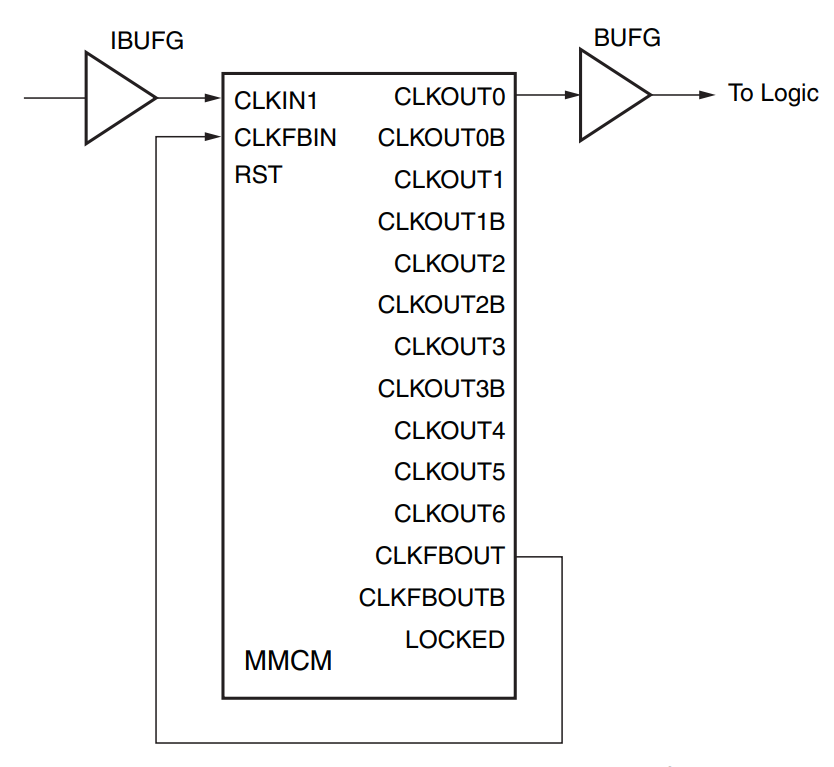
\includegraphics[width=0.5\textwidth]{image/MMCM_INT.PNG}
	\caption{Схема подключения примитива MMCM с внутренней обратной связью}
	\label{fig::MMCM_INT}
\end{figure}

Перейдём к режим работы MMCM. Всего существует два режима работы MMCM: с внутренней и внешней обратной связью. Использование внешней обратной связи нужно если необходимо синхронизация фазы выходных тактовых сигналов со входным. Использование внутренней обратной связи возможно в том случае, если MMCM используется в качестве синтезатора частот или фильтра фазового дрожания, и нет требуемого соотношения фаз между входным тактовым сигналом MMCM и выходным тактовым сигналом MMCM. Производительность MMCM увеличивается, потому что тактовая частота обратной связи не подвержена шуму от источника питания ядра, поскольку он никогда не проходит через блок, питаемый от этого источника. Конечно, шум, вносимый в сигнал CLKIN и BUFG, все равно будет присутствовать. Будем использовать режим с внутренней обратной связью, так как нам не требуется синхронизация фаз входного и выходных тактовых сигналов. На рисунке~\ref{fig::MMCM_INT} представлена схема подключения примитива MMCM с внутренней обратной связью. 

Кроме того, заметим, что входной тактовый сигнал поступает на ПЛИС по дифференциальной паре \verb|clk_in_p|, \verb|clk_in_n|, поэтому для подключения его к примитиву MMCM подребуеться использовать буфер  IBUFGDS, который преобразует дифференциальный тактовый сигнал в обычный("Single-ended")

Обратимся к Vivado Design Suite 7 Series FPGA Libraries Guide для получения Verilog кода подключения \verb|MMCM2_BASE| в наш проект:

\begin{Verbatim}[tabsize=4]
MMCME2_BASE #(
	.BANDWIDTH("OPTIMIZED"),
	.CLKFBOUT_MULT_F(5.0),
	.CLKFBOUT_PHASE(0.0), 
	.CLKIN1_PERIOD(0.0),
	.CLKOUT1_DIVIDE(1),
	.CLKOUT2_DIVIDE(1),
	.CLKOUT3_DIVIDE(1),
	.CLKOUT4_DIVIDE(1),
	.CLKOUT5_DIVIDE(1),
	.CLKOUT6_DIVIDE(1),
	.CLKOUT0_DIVIDE_F(1.0),
	.CLKOUT0_DUTY_CYCLE(0.5),
	.CLKOUT1_DUTY_CYCLE(0.5),
	.CLKOUT2_DUTY_CYCLE(0.5),
	.CLKOUT3_DUTY_CYCLE(0.5),
	.CLKOUT4_DUTY_CYCLE(0.5),
	.CLKOUT5_DUTY_CYCLE(0.5),
	.CLKOUT6_DUTY_CYCLE(0.5),
	.CLKOUT0_PHASE(0.0),
	.CLKOUT1_PHASE(0.0),
	.CLKOUT2_PHASE(0.0),
	.CLKOUT3_PHASE(0.0),
	.CLKOUT4_PHASE(0.0),
	.CLKOUT5_PHASE(0.0),
	.CLKOUT6_PHASE(0.0),
	.CLKOUT4_CASCADE("FALSE"),
	.DIVCLK_DIVIDE(1), 
	.REF_JITTER1(0.0),
	.STARTUP_WAIT("FALSE")
)
MMCME2_BASE_inst (
	.CLKOUT0(CLKOUT0), 
	.CLKOUT0B(CLKOUT0B), 
	.CLKOUT1(CLKOUT1),
	.CLKOUT1B(CLKOUT1B), 	
	.CLKOUT2(CLKOUT2), 		
	.CLKOUT2B(CLKOUT2B), 	
	.CLKOUT3(CLKOUT3), 		
	.CLKOUT3B(CLKOUT3B), 	
	.CLKOUT4(CLKOUT4), 
	.CLKOUT5(CLKOUT5), 
	.CLKOUT6(CLKOUT6), 
	.CLKFBOUT(CLKFBOUT), 
	.CLKFBOUTB(CLKFBOUTB), 
	.LOCKED(LOCKED), 
	.CLKIN1(CLKIN1), 
	.PWRDWN(PWRDWN), 
	.RST(RST), 
	.CLKFBIN(CLKFBIN)
);

\end{Verbatim}

В результате получим следующий код для входного модуля и подключения в нём примитива MMCM:

\begin{Verbatim}[tabsize=4]
`timescale 1ns/1ps

module top_pwm(
    // Clock
    input wire rst,
    // input clk
    input wire clk_in_p,           
    input wire clk_in_n,
    // leds
    output wire led,
    // PWM Fan controller
    output wire pwm
);

// Clock and reset
wire clk_200mhz_ibufg;

// Internal 50 MHz clock
wire clk_mmcm_out;
wire clk_int;
wire rst_int;

wire mmcm_rst = rst;
wire mmcm_locked;
wire mmcm_clkfb;

IBUFGDS
clk_200mhz_ibufgds_inst(
    .I(clk_in_p),
    .IB(clk_in_n),
    .O(clk_200mhz_ibufg)
);

// MMCM instance
// 200 MHz in, 25 MHz out
// M = 5, D = 1 sets Fvco = 1000 MHz (in range)
// Divide by 40 to get output frequency of 25 MHz
MMCME2_BASE #(
    .BANDWIDTH("OPTIMIZED"),
    .CLKOUT0_DIVIDE_F(40),
    .CLKOUT0_DUTY_CYCLE(0.5),
    .CLKOUT0_PHASE(0),
    .CLKOUT1_DIVIDE(8),
    .CLKOUT1_DUTY_CYCLE(0.5),
    .CLKOUT1_PHASE(0),
    .CLKOUT2_DIVIDE(1),
    .CLKOUT2_DUTY_CYCLE(0.5),
    .CLKOUT2_PHASE(0),
    .CLKOUT3_DIVIDE(1),
    .CLKOUT3_DUTY_CYCLE(0.5),
    .CLKOUT3_PHASE(0),
    .CLKOUT4_DIVIDE(1),
    .CLKOUT4_DUTY_CYCLE(0.5),
    .CLKOUT4_PHASE(0),
    .CLKOUT5_DIVIDE(1),
    .CLKOUT5_DUTY_CYCLE(0.5),
    .CLKOUT5_PHASE(0),
    .CLKOUT6_DIVIDE(1),
    .CLKOUT6_DUTY_CYCLE(0.5),
    .CLKOUT6_PHASE(0),
    .CLKFBOUT_MULT_F(5),
    .CLKFBOUT_PHASE(0),
    .DIVCLK_DIVIDE(1),
    .REF_JITTER1(0.010),
    .CLKIN1_PERIOD(5.0),
    .STARTUP_WAIT("FALSE"),
    .CLKOUT4_CASCADE("FALSE")
)
clk_mmcm_inst (
    .CLKIN1(clk_200mhz_ibufg),
    .CLKFBIN(mmcm_clkfb),
    .RST(mmcm_rst),
    .PWRDWN(1'b0),
    .CLKOUT0(clk_mmcm_out),
    .CLKOUT0B(),
    .CLKOUT1(),
    .CLKOUT1B(),
    .CLKOUT2(),
    .CLKOUT2B(),
    .CLKOUT3(),
    .CLKOUT3B(),
    .CLKOUT4(),
    .CLKOUT5(),
    .CLKOUT6(),
    .CLKFBOUT(mmcm_clkfb),
    .CLKFBOUTB(),
    .LOCKED(mmcm_locked)
);

BUFG
clk_bufg_inst (
    .I(clk_mmcm_out),
    .O(clk_int)
);

assign rst_int = ~mmcm_locked;
\end{Verbatim}

Перейдём к разработе ШИМ-контраллера скорости вентилятора. Пусть частота ШИМ-сигнала у нас будет равна 10 кГц. Для получения сигнала с такой частотой напишем счётчик, который поделит наш входной тактовый сигнал частотой равной 25 МГц на величину равную 2500. Код счётчика представлен ниже.

\begin{Verbatim}[tabsize=4]

`timescale 1ns / 1ps

module pwm (
    input clk,
    input rst,
    output pwm
);

reg [15:0] counter_r;

always @(posedge clk) begin 
    if(rst) begin
        counter_r <= 16'b0;
    end else if(counter_r == 'd2499) begin
        counter_r <= 16'b0;
    end else begin
        counter_r <= counter_r + 1;
    end
end

endmodule 

\end{Verbatim}

Для получения широтно-импульсной модуляции введём параметер d. Используя оператор непрервыного присваивания подключим выход \verb|pwm| к компаратору. Теперь при изменении параметра d в диапазоне от 0 до 2500 коэффициент заполнения ШИМ-сигнала будет изменятся в диапазоне от 0 \% до 100 \%. Код ШИМ-контроллера предствлен ниже.

\begin{Verbatim}[tabsize=4]

`timescale 1ns / 1ps

module pwm (
    input clk,
    input rst,
    output pwm
);

reg [15:0] counter_r;

parameter integer d = 1250; 

assign pwm = (d > counter_r) ? 1 : 0; 

always @(posedge clk) begin 
    if(rst) begin
        counter_r <= 16'b0;
    end else if(counter_r == 'd2499) begin
        counter_r <= 16'b0;
    end else begin
        counter_r <= counter_r + 1;
    end
end

endmodule 

\end{Verbatim}

В итоге получаем следующий код, реализующий ШИМ-контроллер:

\begin{Verbatim}[tabsize=4]
`timescale 1ns/1ps

module top_pwm(
    input wire rst,
    // input clk
    input wire clk_in_p,           
    input wire clk_in_n,
    // leds
    output wire led,
    // PWM Fan controller
    output wire pwm
);

// Clock and reset
wire clk_200mhz_ibufg;

// Internal 50 MHz clock
wire clk_mmcm_out;
wire clk_int;
wire rst_int;

wire mmcm_rst = rst;
wire mmcm_locked;
wire mmcm_clkfb;

IBUFGDS
clk_200mhz_ibufgds_inst(
    .I(clk_in_p),
    .IB(clk_in_n),
    .O(clk_200mhz_ibufg)
);

// MMCM instance
// 200 MHz in, 25 MHz out
// M = 5, D = 1 sets Fvco = 1000 MHz (in range)
// Divide by 40 to get output frequency of 25 MHz
MMCME2_BASE #(
    .BANDWIDTH("OPTIMIZED"),
    .CLKOUT0_DIVIDE_F(40),
    .CLKOUT0_DUTY_CYCLE(0.5),
    .CLKOUT0_PHASE(0),
    .CLKOUT1_DIVIDE(8),
    .CLKOUT1_DUTY_CYCLE(0.5),
    .CLKOUT1_PHASE(0),
    .CLKOUT2_DIVIDE(1),
    .CLKOUT2_DUTY_CYCLE(0.5),
    .CLKOUT2_PHASE(0),
    .CLKOUT3_DIVIDE(1),
    .CLKOUT3_DUTY_CYCLE(0.5),
    .CLKOUT3_PHASE(0),
    .CLKOUT4_DIVIDE(1),
    .CLKOUT4_DUTY_CYCLE(0.5),
    .CLKOUT4_PHASE(0),
    .CLKOUT5_DIVIDE(1),
    .CLKOUT5_DUTY_CYCLE(0.5),
    .CLKOUT5_PHASE(0),
    .CLKOUT6_DIVIDE(1),
    .CLKOUT6_DUTY_CYCLE(0.5),
    .CLKOUT6_PHASE(0),
    .CLKFBOUT_MULT_F(5),
    .CLKFBOUT_PHASE(0),
    .DIVCLK_DIVIDE(1),
    .REF_JITTER1(0.010),
    .CLKIN1_PERIOD(5.0),
    .STARTUP_WAIT("FALSE"),
    .CLKOUT4_CASCADE("FALSE")
)
clk_mmcm_inst (
    .CLKIN1(clk_200mhz_ibufg),
    .CLKFBIN(mmcm_clkfb),
    .RST(mmcm_rst),
    .PWRDWN(1'b0),
    .CLKOUT0(clk_mmcm_out),
    .CLKOUT0B(),
    .CLKOUT1(),
    .CLKOUT1B(),
    .CLKOUT2(),
    .CLKOUT2B(),
    .CLKOUT3(),
    .CLKOUT3B(),
    .CLKOUT4(),
    .CLKOUT5(),
    .CLKOUT6(),
    .CLKFBOUT(mmcm_clkfb),
    .CLKFBOUTB(),
    .LOCKED(mmcm_locked)
);

BUFG
clk_bufg_inst (
    .I(clk_mmcm_out),
    .O(clk_int)
);

assign rst_int = ~mmcm_locked;

reg led_r;

assign led = led_r;

always @(posedge clk_int) begin : proc_led
    if(rst_int) begin
        led_r <= 0;
    end else beginB
        led_r <= 1'b1;
    end
end

pwm
pwm_inst 
(
    .clk(clk_int),
    .rst(rst_int),
    .pwm(pwm)
);

endmodule : top_pwm
\end{Verbatim}

Напишем тестбенч для моделирования схемы:

\begin{Verbatim}[tabsize=4]
`timescale 1ns/1ps

module pwm_tb();

    reg sys_clk;
    reg sys_rst;

    initial 
        sys_clk = 1'b0;
    always 
        sys_clk = #(20) ~sys_clk;

    initial begin
        sys_rst = 1'b1;
        #20000
        sys_rst = 1'b0;
    end

    pwm
    pwm_inst
    (
        .clk(sys_clk),
        .rst(sys_rst),
        .pwm()
    );

endmodule
\end{Verbatim}

Напишем файл ограничений для нашего проекта. В этом файле обязательно нужно указать подключение порта светодиода, 
подключение дифференциальной пары тактового сигнала, а также указать величину частоты 
тактового сигнала для временного анализа в Vivado, с помощью команды \verb|create_clock|. Полученный код файла ограничений 
предаставлен ниже. 

\begin{Verbatim}[tabsize=4]
set_property PACKAGE_PIN E19 [get_ports clk_in_p]
set_property IOSTANDARD LVDS [get_ports clk_in_p]
set_property PACKAGE_PIN E18 [get_ports clk_in_n]
set_property IOSTANDARD LVDS [get_ports clk_in_n]

set_property PACKAGE_PIN AV40 [get_ports rst]
set_property IOSTANDARD LVCMOS18 [get_ports rst]

set_property PACKAGE_PIN AM39 [get_ports led]
set_property IOSTANDARD LVCMOS18 [get_ports led]

set_property PACKAGE_PIN BA37 [get_ports pwm]
set_property IOSTANDARD LVCMOS18 [get_ports pwm]

create_clock 	-period 5.000 
				-name sys_clk 
			  	-waveform {0.000 2.500} [get_ports clk_in_p]
\end{Verbatim}

\newpage

Задание:

\begin{enumerate}
	\item
	\item 
	\item 
	\item 
\end{enumerate}

\chapter{Лабораторная работа №3. Реализация конечного автомата для управления ЖКИ}

\section{Протокол работы с ЖКИ S162D}

Индикатор ЖКИ S162D (рис. ~\ref{LCD1602}) позволяет одновременно отображать две строки по 16 символов, при этом каждый символ отображается с помощью матрицы точек 5х8. 

\begin{figure}[!ht]
	\centering
	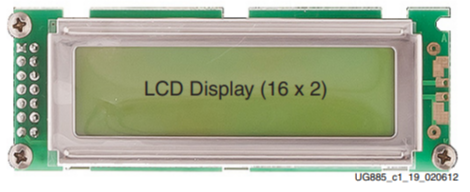
\includegraphics[width=0.4\textwidth]{image/LCD1602.PNG}
	\caption{Внешний вид индикатора S162D}
	\label{LCD1602}
\end{figure}

\begin{table}[!ht]
	\begin{center}
		\begin{tabular}{c c}
			\hline\hline
			Вывод & Назначение \\
			\hline
			VDD & Вывод питания \\
			VSS & Вывод земли \\
			VO & Установка контраста \\
			RS & Сигнал выбора регистра \\
			R/W & Лог. 1 – чтение модуля,лог. 0 – запись в модуль \\
			E & Сигнал выбора модуля \\
			DB0 & Линия информационной шины \\
			DB1 & Линия информационной шины \\
			DB2 & Линия информационной шины \\
			DB3 & Линия информационной шины \\
			DB4 & Линия информационной шины \\
			DB5 & Линия информационной шины \\
			DB6 & Линия информационной шины \\
			DB7 & Линия информационной шины \\
			\hline
		\end{tabular}
		\caption{Выводы индикатора}
		\label{LCD_PIN}
	\end{center}
\end{table}

Выводы VDD и VSS необходимы для подачи питания на индикатор, 
вывод VO служит для настройки контрастности индикатора. Обычно к 
нему подключается скользящий контакт потенциометра на 10-20 
кОм, включенного между линиями питания и земли. Однако при 
известных номиналах можно заменить его обычным резисторным 
делителем

Передача информации на контроллер ЖКИ осуществляется по 
параллельной шине данных DB0…DB7. 
По ней передаются как команды контроллеру, так и коды выводимых символов. 
Вид передаваемой информации (команды или данные) задается 
с помощью вывода 4 (RS): при низком уровне на данном выводе 
контроллер воспринимает принятую информацию как команду, при высоком – как данные. 
Для синхронизации передачи служит вывод 6 (Е) – 
информация с шины данных записывается во входной регистр контроллера 
по спаду сигнала на данном выводе.

Контроллер ЖКИ не только принимает информацию, но и может 
ее передавать – режим чтение/запись устанавливается с помощью 
вывода 5 (R/W): при низком уровне на данном выводе происходит 
запись в контроллер, при высоком – чтение.

\begin{table}[!ht]
	\begin{center}
		\begin{tabular}{c c c c c}
			\hline\hline
			FPGA (U1) Pin & Net Name &  I/O Standard & LCD Header Pin(J31) \\
			\hline
			AT42 & \verb|LCD_DB4_LS| & LVCMOS18 & 4 \\
			AR38 & \verb|LCD_DB5_LS| & LVCMOS18 & 3 \\
			AR39 & \verb|LCD_DB6_LS| & LVCMOS18 & 2 \\
			AN40 & \verb|LCD_DB7_LS| & LVCMOS18 & 1 \\
			AR42 & \verb|LCD_RW_LS| & LVCMOS18 & 10 \\
			AN41 & \verb|LCD_RS_LS| & LVCMOS18 & 11 \\
			AT40 & \verb|LCD_E_LS| & LVCMOS18 & 9 \\
			\hline
		\end{tabular}
		\caption{Подключение индикатора к ПЛИС}
		\label{LCD_TO_FPGA}
	\end{center}
\end{table}

Таким образом, для подключения индикатора к управляющему 
контроллеру необходимо использовать 11 выводов. Для уменьшения 
данного количества возможна работа ЖКИ с 4-проводной шиной 
данных – к ЖКИ подключаются только выводы DB7…DB4, при 
этом передача байта на ЖКИ происходит в два этапа: сначала передаются биты DB7…DB4, затем DB3…DB0. Количество используемых выводов контроллера уменьшается до 7.

Последовательности действий, которые необходимо выполнить 
управляющей системе при совершении операций записи и чтения 
для 4-разрядной шин приведены ниже.

\begin{figure}[!ht]
	\centering
	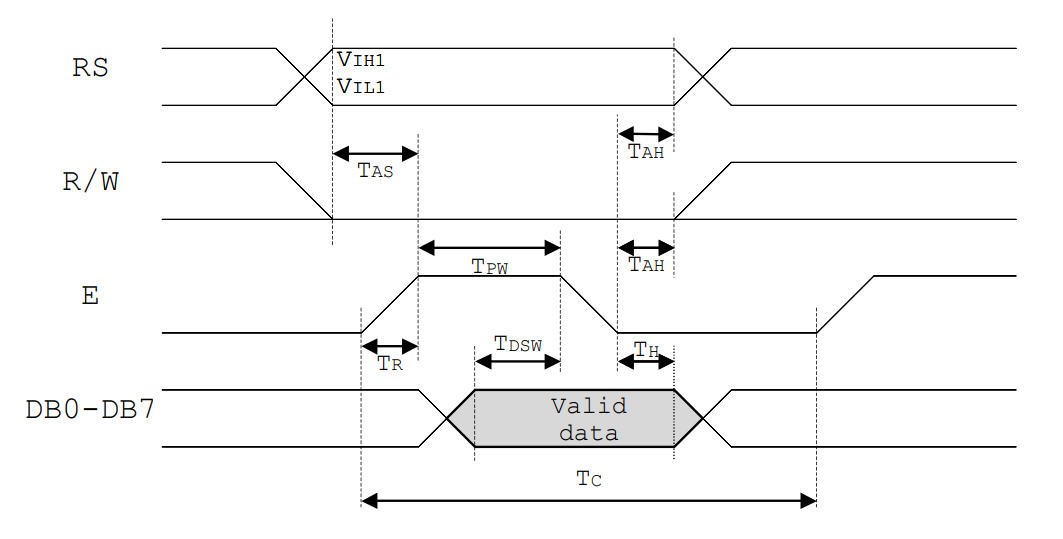
\includegraphics[width=0.7\textwidth]{image/LCD_WR_2.PNG}
	\caption{Временная диаграмма операции записи}
	\label{full_adder}
\end{figure}

\begin{table}[!ht]
	\begin{center}
		\begin{tabular}{c c c c c}
			\hline\hline
			Параметр 							& Обозн. 	& Мин. 	& Макс. \\
			\hline
			Enable Cycle Time, Pin E 			& tC		& 400 	& 	- 	\\
			Enable Pulse Width Pin E 			& tPW 		& 150 	& 	- 	\\
			Enable Rise/Fall Time Pin E 		& tR/tF 	& - 	& 	25	\\
			Address Setup Time Pins: RS,RW,E 	& tAS 		& 30 	& 	-	\\
			Address Hold Time Pins: RS,RW,E 	& tAH 		& 10 	& 	-	\\
			Data Setup Time Pins: DB0 - DB7 	& tDSW 		& 40 	& 	-	\\
			Data Hold Time Pins: DB0 - DB7  	& tH 		& 10 	& 	-	\\
			\hline
		\end{tabular}
		\caption{Временные характеристики сигналов при записи (нс)}
		\label{LCD_TO_FPGA_WR_TABLE}
	\end{center}
\end{table}

Операции записи для 4-разрядной шины:
\begin{enumerate}
	\item Установить значение линии RS.
	\item Вывести значение старшей тетрады байта данных на линии шины DB4...DB7.
	\item Установить линию Е = 1.
	\item Установить линию Е = 0.
	\item Вывести значение младшей тетрады байта данных на линии шины DB4...DB7.
	\item Установить линию Е = 1.
	\item Установить линию Е = 0.
	\item Установить линии шины DB0...DB7 = HiZ.
\end{enumerate}

\begin{figure}[!ht]
	\centering
	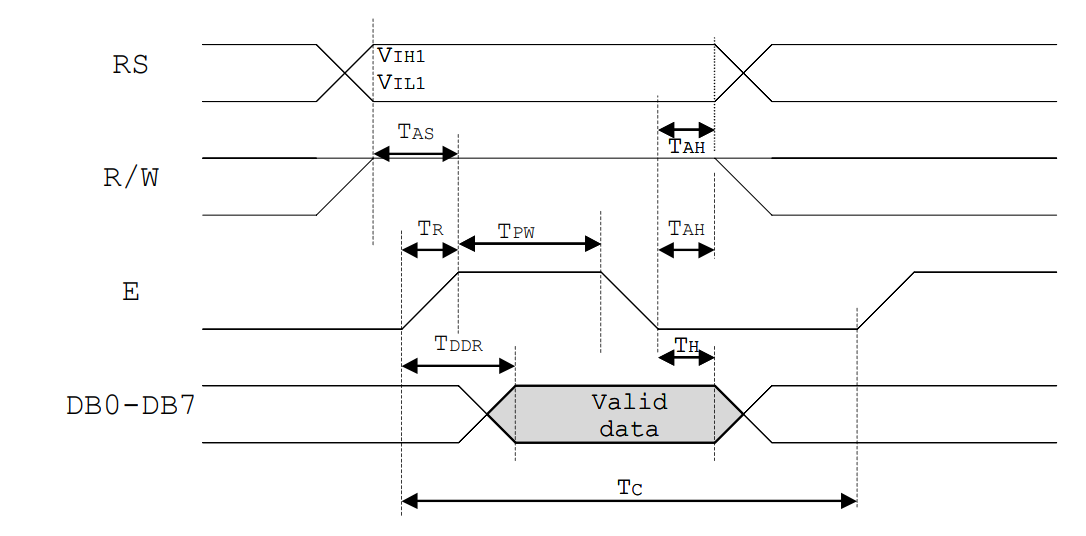
\includegraphics[width=0.7\textwidth]{image/LCD_READ_2.PNG}
	\caption{Временная диаграмма операции чтения}
	\label{full_adder}
\end{figure}

\begin{table}[!ht]
	\begin{center}
		\begin{tabular}{c c c c c}
			\hline\hline
			Параметр 							& Обозн. 	& Мин. 	& Макс. \\
			\hline
			Enable Cycle Time, Pin E 			& tC		& 400 	& 	- 	\\
			Enable Pulse Width Pin E 			& tPW 		& 150 	& 	- 	\\
			Enable Rise/Fall Time Pin E 		& tR/tF 	& - 	& 	25	\\
			Address Setup Time Pins: RS,RW,E 	& tAS 		& 30 	& 	-	\\
			Address Hold Time Pins: RS,RW,E 	& tAH 		& 10 	& 	-	\\
			Data Setup Time Pins: DB0 - DB7 	& tDSW 		&  - 	& 	100	\\
			Data Hold Time Pins: DB0 - DB7  	& tH 		& 10 	& 	-	\\
			\hline
		\end{tabular}
		\caption{Временные характеристики сигналов при чтении(нс)}
		\label{LCD_TO_FPGA_RD_TABLE}
	\end{center}
\end{table}

Операции чтения для 4-разрядной шины:
\begin{enumerate}
	\item Установить значение линии RS.
	\item Установить линию R/W = 1.
	\item Установить линию Е = 1.
	\item Считать значение старшей тетрады байта данных с линий шины DB4...DB7.
	\item Установить линию Е = 0.
	\item Установить линию Е = 1.
	\item Считать значение младшей тетрады байта данных с линий шины DB4...DB7.
	\item Установить линию Е = 0.
	\item Установить линию R/W = 0.
\end{enumerate}

Приведенные операции подразумевают, что время выполнения 
каждого шага составляет не менее 250 нс. 

Описанные операции записи/чтения байта являются базовыми 
для осуществления обмена данными с ЖКИ модулем.

В техническом описании на контроллер ЖКИ приведены алгоритмы инициализации индикатора для различных вариантов его 
подключения. Рассмотрим алгоритм инициализации для подключения по 4-проводной шине данных. Он состоит из следующих этапов:
\begin{enumerate}
	\item При включении ожидание не менее 40 мс после того момента, как напряжение питания превысит 2,7 В.
	\item Отправка команды 0x30.
	\item Ожидание не менее 4,1 мс.
	\item Отправка команды 0х30.
	\item Ожидание не менее 100 мкс.
	\item Отправка команды 0х30. После данной команды контроллер 
выходит на нормальный режим работы: может выполнять данные 
ему инструкции и сигнализировать об их выполнении флагом BF.
	\item  При включении ЖКИ по умолчанию настроен на работу с 8-
разрядной шиной данных, поэтому в первую очередь необходимо 
установить 4-разрядный режим путем установки флага D/L в ноль 
командой 0х20. После данной команды все передачи по шине данных будут проходить в 2 этапа: сначала передача старшей тетрады, 
затем – младшей.
	\item Отправка команды 0х28 – данная команда установит значения флагов N и F таким образом, что ЖКИ будет настроен на отображение двух строк с матрицами символов 5х8 точек
	\item Отправка команды 0х0С – установка значений флагов D, C, 
B – включение отображения на дисплей, символы курсоров не отображаются.
	\item  Отправка команды 0х06 – установка значений флагов I/D и S
– настройка счетчика адреса АС на увеличение при записи символа, 
выключение сдвига экрана при записи.
\end{enumerate}

После выполнения данной последовательности работа с дисплеем заключается в записи по определенным адресам кодов символов, которые необходимо вывести на экран. При приведенных выше настройках при отправке в ЖКИ кода символа он отображается в 
том месте экрана, на которое указывает счетчик АС, – после инициализации он указывает на первый символ первой строки. После записи символа значение счетчика автоматически увеличивается, и он начинает указывать на второй символ. При записи последнего символа первой строки АС автоматически начинает указывать на первый символ второй.

Для непосредственного указания, какой символ требуется переписать, управляющий контроллер отправляет команду, содержащую 
новый адрес АС. Так, адрес первого символа первой строки – 0х00, 
второго – 0х01 и т. д. Однако адреса второй строки, вне зависимости 
от количества знакомест в строке ЖКИ, начинаются с адреса 0х40. 
Далее – 0х41, 0х42 и так по порядку

\section{Разработка конечного автомата для управления ЖКИ}

Изучив основные команды управления ЖКИ и алгоритм его инициализации приступим к разработке модуля упрвления индикатором на языке Verilog. 
Создадим модуль верхнего уровня, который будет генерировать тактовый сигнал требуемой частоты, а также формировать сброс для модуля управления ЖКИ. Используемый тактовый сигнал имеет частоту 200 МГц, 
модуль управления ЖКИ будем тактировать частотой в 50 МГц. Для снижения частоты 
используем примитив \verb|MMCME2_BASE|. Сброс модуля управления ЖКИ будем проводить отслеживая сигнал \verb|LOCKED| примитива \verb|MMCME2_BASE|. 

Входными сигналами модуля будут:
\begin{enumerate}
	\item тактовый сигнал, частотой 200 МГц, который поступает на ПЛИС по дифференциальной паре: \verb|clk_in_n|,\verb|clk_in_p|;
	\item cигнал асинхронного сброса: \verb|rst|.
\end{enumerate}

Выходными сигналами модуля будут: 
\begin{enumerate}
	\item шина данных - \verb|lcd_data|, состоящая из 4 проводов: DB4, DB5, DB6, DB7;  
	\item сигналы управления ЖКИ: \verb|lcd_e|, \verb|lcd_rs|, \verb|lcd_rw|;
	\item сигнал \verb|led| для управления одним светодиодом, предназначен для индикации пристутсвия сигнала сброса и тактового сигнала.
\end{enumerate}

\begin{Verbatim}[tabsize=4]
`timescale 1ns/1ps

module top_lcd(
	// reset
    input wire rst,
    // input clk
    input wire clk_in_p,           
    input wire clk_in_n,
    // leds
	output wire led,
	// LCD data bus
	output wire [3:0] lcd_data, 
	// LCD: E   (control bit)	
	output wire lcd_e,	
	// LCD: RS  (setup or data)
	output wire lcd_rs,	
	// LCD: R/W (read or write)
	output wire lcd_rw	
);

endmodule : top_lcd
\end{Verbatim}

\begin{Verbatim}[tabsize=4]
lcd #(
	.CYCLES_PER_US(50)
)
lcd_inst
(
	.clk(clk_int),  
	.rst(rst_int),  
	.ctrl_lcd({lcd_rs,lcd_rw,lcd_e}),
	.data_lcd(lcd_data)
);
\end{Verbatim}

Создадим модуль, который будет управлять ЖКИ. Входными сигналами модуля будут: тактовый сигнал, сигнал сброса.
Выходными сигналами модуля будут: 
\begin{enumerate}
	\item Шина данных, состоящая из 4 проводов: DB4, DB5, DB6, DB7.  
	\item Шина управления ЖКИ, состоящая из трёх проводов: RS, RW, E.
\end{enumerate}

Также введём параметризацию модуля с помощью параметра \verb|CYCLES_PER_US|, который 
означает число периодов тактового сигнала необходимых для получения задержки
в одну микросекунду. 

\begin{Verbatim}[tabsize=4]

`timescale 1ns/1ps

module lcd #(
	parameter CYCLES_PER_US = 50
)
(
	input wire clk,    
	input wire rst, 
	output wire [2:0] ctrl_lcd,
	output wire [3:0] data_lcd
);
\end{Verbatim}

\begin{Verbatim}[tabsize=4]
	localparam [3:0]
		WAITING = 4'd0,
        INIT_H30_ONE = 4'd1,
        INIT_H30_TWO = 4'd2,
        INIT_H30_THREE = 4'd3,
        INIT_H20 = 4'd4,
        INIT_FUNCTION_SET = 4'd5,
        INIT_DISPLAY_ON = 4'd6,
		INIT_DISPLAY_CLEAR = 4'd7,
		INIT_SET_ENTRY_MODE = 4'd8,
		CUR_FIRST_ROW = 4'd9,
		WRITE_UPPER_LINE = 4'd10,
		COUNTER_UPPER_LINE = 4'd11,
		CUR_SECOND_ROW = 4'd12,
		WRITE_LOWER_LINE = 4'd13,
		COUNTER_LOWER_LINE = 4'd14,
		DONE = 4'd15;
\end{Verbatim}

\begin{Verbatim}[tabsize=4]
	reg [3:0] lcd_state_r;		
	reg [2:0] ctrl_lcd_r; 
	reg [3:0] data_lcd_r;
	
	reg [31:0] counter_r;
	reg [3:0] counter_upper_line_r;
	reg [3:0] counter_lower_line_r;

	reg [7:0] upper_line [15:0];
	reg [7:0] lower_line [15:0];
\end{Verbatim}

\begin{Verbatim}[tabsize=4]
	parameter integer wait__1us = 1 * CYCLES_PER_US;
	parameter integer wait__2us = 2 * CYCLES_PER_US;    // 10us 
	parameter integer wait__3us = 3 * CYCLES_PER_US;    // 20us 
	parameter integer wait__4us = 4 * CYCLES_PER_US;    // 40us 
	parameter integer wait__200us = 200 * CYCLES_PER_US; // 5ms

	parameter integer wait__dispay_clear = 3000 * CYCLES_PER_US; // 1.52ms 
	parameter integer wait__power_on = 15000 * CYCLES_PER_US; // 45ms 

	parameter integer wait__init_h30_one = 5000 * CYCLES_PER_US; // 5ms 
	parameter integer wait__init_h30_two = 500 * CYCLES_PER_US; // 5ms
\end{Verbatim}

\begin{Verbatim}[tabsize=4]
	assign ctrl_lcd = ctrl_lcd_r; // {RS, RW, E} 2, 1, 0
	assign data_lcd = data_lcd_r;
\end{Verbatim}

\begin{Verbatim}[tabsize=4]
	initial begin
		upper_line[0] = 8'h46; // F
		upper_line[1] = 8'h69; // i
		upper_line[2] = 8'h72; // r
		upper_line[3] = 8'h6d; // m
		upper_line[4] = 8'h77; // w
		upper_line[5] = 8'h61; // a
		upper_line[6] = 8'h72; // r
		upper_line[7] = 8'h65; // e
		upper_line[8] = 8'h20; // 
		upper_line[9] = 8'h6c; // l
		upper_line[10] = 8'h6f; // o
		upper_line[11] = 8'h61; // a
		upper_line[12] = 8'h64; // d
		upper_line[13] = 8'h65; // e
		upper_line[14] = 8'h64; // d
		upper_line[15] = 8'h21; // !
				
		lower_line[0] = 8'h30; // 0
		lower_line[1] = 8'h31; // 1
		lower_line[2] = 8'h32; // 2
		lower_line[3] = 8'h33; // 3
		lower_line[4] = 8'h34; // 4
		lower_line[5] = 8'h35; // 5
		lower_line[6] = 8'h36; // 6
		lower_line[7] = 8'h37; // 7
		lower_line[8] = 8'h38; // 8
		lower_line[9] = 8'h39; // 9
		lower_line[10] = 8'h61; // a
		lower_line[11] = 8'h62; // b
		lower_line[12] = 8'h63; // c
		lower_line[13] = 8'h64; // d
		lower_line[14] = 8'h65; // e
		lower_line[15] = 8'h66; // f
	end
\end{Verbatim}

\begin{Verbatim}[tabsize=4]
    always @(posedge clk) begin
        if (rst) begin
        	lcd_state_r <= WAITING;
        	ctrl_lcd_r <= 3'b0;
        	data_lcd_r <= 4'b0;
        	counter_r <= 32'b0;
        	counter_upper_line_r <= 4'b0;
			counter_lower_line_r <= 4'b0;
        end else begin
        	case (lcd_state_r)
        	// Здесь будем описывать конечный автомат
        	endcase
        end
    end
\end{Verbatim}

\begin{Verbatim}[tabsize=4]
WAITING: begin 
	if(counter_r >= wait__power_on) begin
       	lcd_state_r <= INIT_H30_ONE;
          	counter_r <= 32'b0;
    end else begin
   		counter_r <= counter_r + 1;
      	lcd_state_r <= WAITING;
   	end
end
\end{Verbatim}

\begin{Verbatim}[tabsize=4]
INIT_H30_ONE: begin // 0x30
	data_lcd_r <= 4'b0011;
	if(counter_r >= wait__init_h30_one) begin
		counter_r <= 32'b0;
		lcd_state_r <= INIT_H30_TWO;
	end else if(counter_r < wait__init_h30_one && counter_r >= wait__1us) begin
		counter_r <= counter_r + 1;
		ctrl_lcd_r <= 3'b000;
		lcd_state_r <= INIT_H30_ONE;
	end else begin
		counter_r <= counter_r + 1;
		ctrl_lcd_r <= 3'b001;
		lcd_state_r <= INIT_H30_ONE;
	end
end
\end{Verbatim}

\begin{Verbatim}[tabsize=4]
INIT_H30_TWO: begin // 0x30
   	data_lcd_r <= 4'b0011;
   	if(counter_r >= wait__init_h30_two) begin
   		counter_r <= 32'b0;
   		lcd_state_r <= INIT_H30_THREE;
   	end else if(counter_r < wait__init_h30_two && counter_r >= wait__1us) begin
   		counter_r <= counter_r + 1;
   		ctrl_lcd_r <= 3'b000;
   		lcd_state_r <= INIT_H30_TWO;
   	end else begin
   		counter_r <= counter_r + 1;
   		ctrl_lcd_r <= 3'b001;
   		lcd_state_r <= INIT_H30_TWO;
   	end
end
\end{Verbatim}

\begin{Verbatim}[tabsize=4]
INIT_H30_TWO: begin // 0x30
   	data_lcd_r <= 4'b0011;
   	if(counter_r >= wait__init_h30_two) begin
   		counter_r <= 32'b0;
   		lcd_state_r <= INIT_H30_THREE;
   	end else if(counter_r < wait__init_h30_two && counter_r >= wait__1us) begin
   		counter_r <= counter_r + 1;
   		ctrl_lcd_r <= 3'b000;
   		lcd_state_r <= INIT_H30_TWO;
   	end else begin
   		counter_r <= counter_r + 1;
   		ctrl_lcd_r <= 3'b001;
   		lcd_state_r <= INIT_H30_TWO;
   	end
end
\end{Verbatim}

\begin{Verbatim}[tabsize=4]
INIT_H30_THREE: begin // 0x30
	data_lcd_r <= 4'b0011;
	if(counter_r >= wait__200us) begin
		counter_r <= 32'b0;
		lcd_state_r <= INIT_H20;
	end else if(counter_r < wait__200us && counter_r >= wait__1us) begin
		counter_r <= counter_r + 1;
		ctrl_lcd_r <= 3'b000;
		lcd_state_r <= INIT_H30_THREE;
	end else begin
		counter_r <= counter_r + 1;
		ctrl_lcd_r <= 3'b001;
		lcd_state_r <= INIT_H30_THREE;
	end
end
\end{Verbatim}

\begin{Verbatim}[tabsize=4]
INIT_H20: begin // 0x20
	data_lcd_r <= 4'b0010;
	if(counter_r >= wait__200us) begin
		counter_r <= 32'b0;
		lcd_state_r <= INIT_FUNCTION_SET;
	end else if(counter_r < wait__200us && counter_r >= wait__1us) begin
		counter_r <= counter_r + 1;
		ctrl_lcd_r <= 3'b000;
		lcd_state_r <= INIT_H20;
	end else begin
		counter_r <= counter_r + 1;
		ctrl_lcd_r <= 3'b001;
		lcd_state_r <= INIT_H20;
	end
end
\end{Verbatim}

\begin{Verbatim}[tabsize=4]
INIT_FUNCTION_SET: begin // 0x28
	if(counter_r < wait__1us) begin
		counter_r <= counter_r + 1;
		data_lcd_r <= 4'b0010;
		ctrl_lcd_r <= 3'b001;
		lcd_state_r <= INIT_FUNCTION_SET;
	end else if(wait__1us <= counter_r && counter_r < wait__2us) begin
		counter_r <= counter_r + 1;
		data_lcd_r <= 4'b0010;
		ctrl_lcd_r <= 3'b000;
		lcd_state_r <= INIT_FUNCTION_SET;
	end else if(wait__2us <= counter_r && counter_r < wait__3us) begin
		counter_r <= counter_r + 1;
		data_lcd_r <= 4'b1000;
		ctrl_lcd_r <= 3'b001;
		lcd_state_r <= INIT_FUNCTION_SET;
	end else if(wait__3us <= counter_r && counter_r < wait__4us) begin
		counter_r <= counter_r + 1;
		data_lcd_r <= 4'b1000;
		ctrl_lcd_r <= 3'b000;
		lcd_state_r <= INIT_FUNCTION_SET;
	end else if(wait__4us <= counter_r && counter_r < wait__200us) begin
		counter_r <= counter_r + 1;
		data_lcd_r <= 4'b0000;
		ctrl_lcd_r <= 3'b000;
		lcd_state_r <= INIT_FUNCTION_SET;
	end else begin
		counter_r <= 32'b0;
		lcd_state_r <= INIT_DISPLAY_ON;
	end
end
\end{Verbatim}

\begin{Verbatim}[tabsize=4]
INIT_DISPLAY_ON: begin // 0x0F
	if(counter_r < wait__1us) begin
		counter_r <= counter_r + 1;
		data_lcd_r <= 4'b0000;
		ctrl_lcd_r <= 3'b001;
		lcd_state_r <= INIT_DISPLAY_ON;
	end else if(wait__1us <= counter_r && counter_r < wait__2us) begin
		counter_r <= counter_r + 1;
		data_lcd_r <= 4'b0000;
		ctrl_lcd_r <= 3'b000;
		lcd_state_r <= INIT_DISPLAY_ON;
	end else if(wait__2us <= counter_r && counter_r < wait__3us) begin
		counter_r <= counter_r + 1;
		data_lcd_r <= 4'b1111;
		ctrl_lcd_r <= 3'b001;
		lcd_state_r <= INIT_DISPLAY_ON;
	end else if(wait__3us <= counter_r && counter_r < wait__4us) begin
		counter_r <= counter_r + 1;
		data_lcd_r <= 4'b1111;
		ctrl_lcd_r <= 3'b000;
		lcd_state_r <= INIT_DISPLAY_ON;
	end else if(wait__4us <= counter_r && counter_r < wait__200us) begin
		counter_r <= counter_r + 1;
		data_lcd_r <= 4'b0000;
		ctrl_lcd_r <= 3'b000;
		lcd_state_r <= INIT_DISPLAY_ON;
	end else begin
		counter_r <= 32'b0;
		lcd_state_r <= INIT_DISPLAY_CLEAR;
	end
end
\end{Verbatim}

\begin{Verbatim}[tabsize=2]
INIT_DISPLAY_CLEAR: begin // 0x01
	if(counter_r < wait__1us) begin
		counter_r <= counter_r + 1;
		data_lcd_r <= 4'b0000;
		ctrl_lcd_r <= 3'b001;
		lcd_state_r <= INIT_DISPLAY_CLEAR;
	end else if(wait__1us <= counter_r && counter_r < wait__2us) begin
		counter_r <= counter_r + 1;
		data_lcd_r <= 4'b0000;
		ctrl_lcd_r <= 3'b000;
		lcd_state_r <= INIT_DISPLAY_CLEAR;
	end else if(wait__2us <= counter_r && counter_r < wait__3us) begin
		counter_r <= counter_r + 1;
		data_lcd_r <= 4'b0001;
		ctrl_lcd_r <= 3'b001;
		lcd_state_r <= INIT_DISPLAY_CLEAR;
	end else if(wait__3us <= counter_r && counter_r < wait__4us) begin
		counter_r <= counter_r + 1;
		data_lcd_r <= 4'b0001;
		ctrl_lcd_r <= 3'b000;
		lcd_state_r <= INIT_DISPLAY_CLEAR;
	end else if(wait__4us <= counter_r 
							&& counter_r < wait__dispay_clear) begin
		counter_r <= counter_r + 1;
		data_lcd_r <= 4'b0000;
		ctrl_lcd_r <= 3'b000;
		lcd_state_r <= INIT_DISPLAY_CLEAR;
	end else begin
		counter_r <= 32'b0;
		lcd_state_r <= INIT_SET_ENTRY_MODE;
	end
end
\end{Verbatim}

\begin{Verbatim}[tabsize=2]
INIT_SET_ENTRY_MODE: begin //0x06
	if(counter_r < wait__1us) begin
		counter_r <= counter_r + 1;
		data_lcd_r <= 4'b0000;
		ctrl_lcd_r <= 3'b001;
		lcd_state_r <= INIT_SET_ENTRY_MODE;
	end else if(wait__1us <= counter_r && counter_r < wait__2us) begin
		counter_r <= counter_r + 1;
		data_lcd_r <= 4'b0000;
		ctrl_lcd_r <= 3'b000;
		lcd_state_r <= INIT_SET_ENTRY_MODE;
	end else if(wait__2us <= counter_r && counter_r < wait__3us) begin
		counter_r <= counter_r + 1;
		data_lcd_r <= 4'b0110;
		ctrl_lcd_r <= 3'b001;
		lcd_state_r <= INIT_SET_ENTRY_MODE;
	end else if(wait__3us <= counter_r && counter_r < wait__4us) begin
		counter_r <= counter_r + 1;
		data_lcd_r <= 4'b0110;
		ctrl_lcd_r <= 3'b000;
		lcd_state_r <= INIT_SET_ENTRY_MODE;
	end else if(wait__4us <= counter_r && counter_r < wait__200us) begin
		counter_r <= counter_r + 1;
		data_lcd_r <= 4'b0000;
		ctrl_lcd_r <= 3'b000;
		lcd_state_r <= INIT_SET_ENTRY_MODE;
	end else begin
		counter_r <= 32'b0;
		lcd_state_r <= CUR_FIRST_ROW;
	end
end
\end{Verbatim}

\begin{Verbatim}[tabsize=4]
CUR_FIRST_ROW: begin // 0x80
	if(counter_r < wait__1us) begin
		counter_r <= counter_r + 1;
		data_lcd_r <= 4'b1000;
		ctrl_lcd_r <= 3'b001;
		lcd_state_r <= CUR_FIRST_ROW;
	end else if(wait__1us <= counter_r && counter_r < wait__2us) begin
		counter_r <= counter_r + 1;
		data_lcd_r <= 4'b1000;
		ctrl_lcd_r <= 3'b000;
		lcd_state_r <= CUR_FIRST_ROW;
	end else if(wait__2us <= counter_r && counter_r < wait__3us) begin
		counter_r <= counter_r + 1;
		data_lcd_r <= 4'b0000;
		ctrl_lcd_r <= 3'b001;
		lcd_state_r <= CUR_FIRST_ROW;
	end else if(wait__3us <= counter_r && counter_r < wait__4us) begin
		counter_r <= counter_r + 1;
		data_lcd_r <= 4'b0000;
		ctrl_lcd_r <= 3'b000;
		lcd_state_r <= CUR_FIRST_ROW;
	end else if(wait__4us <= counter_r && counter_r < wait__200us) begin
		counter_r <= counter_r + 1;
		data_lcd_r <= 4'b0000;
		ctrl_lcd_r <= 3'b000;
		lcd_state_r <= CUR_FIRST_ROW;
	end else begin
		counter_r <= 32'b0;
		lcd_state_r <= WRITE_UPPER_LINE;
	end
end
\end{Verbatim}

\begin{Verbatim}[tabsize=4]
WRITE_UPPER_LINE: begin
	if(counter_r < wait__1us) begin
		counter_r <= counter_r + 1;
		data_lcd_r <= upper_line[counter_upper_line_r][7:4];
		ctrl_lcd_r <= 3'b101;
		lcd_state_r <= WRITE_UPPER_LINE;
	end else if(wait__1us <= counter_r && counter_r < wait__2us) begin
		counter_r <= counter_r + 1;
		data_lcd_r <= upper_line[counter_upper_line_r][7:4];
		ctrl_lcd_r <= 3'b000;
		lcd_state_r <= WRITE_UPPER_LINE;
	end else if(wait__2us <= counter_r && counter_r < wait__3us) begin
		counter_r <= counter_r + 1;
		data_lcd_r <= upper_line[counter_upper_line_r][3:0];;
		ctrl_lcd_r <= 3'b101;
		lcd_state_r <= WRITE_UPPER_LINE;
	end else if(wait__3us <= counter_r && counter_r < wait__4us) begin
		counter_r <= counter_r + 1;
		data_lcd_r <= upper_line[counter_upper_line_r][3:0];;
		ctrl_lcd_r <= 3'b000;
		lcd_state_r <= WRITE_UPPER_LINE;
	end else if(wait__4us <= counter_r && counter_r < wait__200us) begin
		counter_r <= counter_r + 1;
		data_lcd_r <= 4'b0000;
		ctrl_lcd_r <= 3'b000;
		lcd_state_r <= WRITE_UPPER_LINE;
	end else begin
		counter_r <= 32'b0;
		lcd_state_r <= COUNTER_UPPER_LINE;
	end
end
\end{Verbatim}

\begin{Verbatim}[tabsize=4]
COUNTER_UPPER_LINE: begin
	if(counter_upper_line_r == 4'd15) begin
		counter_upper_line_r <= 4'b0;
		lcd_state_r <= CUR_SECOND_ROW;		
	end else begin
    	counter_upper_line_r <= counter_upper_line_r + 1;
    	lcd_state_r <= WRITE_UPPER_LINE;
	end
end
\end{Verbatim}

\begin{Verbatim}[tabsize=4]
CUR_SECOND_ROW: begin
	if(counter_r < wait__1us) begin
		counter_r <= counter_r + 1;
		data_lcd_r <= 4'b1100;
		ctrl_lcd_r <= 3'b001;
		lcd_state_r <= CUR_SECOND_ROW;
	end else if(wait__1us <= counter_r && counter_r < wait__2us) begin
		counter_r <= counter_r + 1;
		data_lcd_r <= 4'b1100;
		ctrl_lcd_r <= 3'b000;
		lcd_state_r <= CUR_SECOND_ROW;
	end else if(wait__2us <= counter_r && counter_r < wait__3us) begin
		counter_r <= counter_r + 1;
		data_lcd_r <= 4'b0000;
		ctrl_lcd_r <= 3'b001;
		lcd_state_r <= CUR_SECOND_ROW;
	end else if(wait__3us <= counter_r && counter_r < wait__4us) begin
		counter_r <= counter_r + 1;
		data_lcd_r <= 4'b0000;
		ctrl_lcd_r <= 3'b000;
		lcd_state_r <= CUR_SECOND_ROW;
	end else if(wait__4us <= counter_r && counter_r < wait__200us) begin
		counter_r <= counter_r + 1;
		data_lcd_r <= 4'b0000;
		ctrl_lcd_r <= 3'b000;
		lcd_state_r <= CUR_SECOND_ROW;
	end else begin
		counter_r <= 32'b0;
		lcd_state_r <= WRITE_LOWER_LINE;
	end
end
\end{Verbatim}

\begin{Verbatim}[tabsize=4]
WRITE_LOWER_LINE: begin
	if(counter_r < wait__1us) begin
		counter_r <= counter_r + 1;
		data_lcd_r <= lower_line[counter_lower_line_r][7:4];
		ctrl_lcd_r <= 3'b101;
		lcd_state_r <= WRITE_LOWER_LINE;
	end else if(wait__1us <= counter_r && counter_r < wait__2us) begin
		counter_r <= counter_r + 1;
		data_lcd_r <= lower_line[counter_lower_line_r][7:4];
		ctrl_lcd_r <= 3'b000;
		lcd_state_r <= WRITE_LOWER_LINE;
	end else if(wait__2us <= counter_r && counter_r < wait__3us) begin
		counter_r <= counter_r + 1;
		data_lcd_r <= lower_line[counter_lower_line_r][3:0];;
		ctrl_lcd_r <= 3'b101;
		lcd_state_r <= WRITE_LOWER_LINE;
	end else if(wait__3us <= counter_r && counter_r < wait__4us) begin
		counter_r <= counter_r + 1;
		data_lcd_r <= lower_line[counter_lower_line_r][3:0];;
		ctrl_lcd_r <= 3'b000;
		lcd_state_r <= WRITE_LOWER_LINE;
	end else if(wait__4us <= counter_r && counter_r < wait__200us) begin
		counter_r <= counter_r + 1;
		data_lcd_r <= 4'b0000;
		ctrl_lcd_r <= 3'b000;
		lcd_state_r <= WRITE_LOWER_LINE;
	end else begin
		counter_r <= 32'b0;
		lcd_state_r <= COUNTER_LOWER_LINE;
	end
end
\end{Verbatim}

\begin{Verbatim}[tabsize=4]
COUNTER_LOWER_LINE: begin
	if(counter_lower_line_r == 32'd15) begin
		counter_lower_line_r <= 32'b0;
		lcd_state_r <= DONE;		
	end else begin
    	counter_lower_line_r <= counter_lower_line_r + 1;
    	lcd_state_r <= WRITE_LOWER_LINE;
	end
end
\end{Verbatim}

\begin{Verbatim}[tabsize=4]
DONE: begin
	lcd_state_r <= DONE;
end
\end{Verbatim}

Напишем файл ограничений для нашего проекта. В этом файле обязательно нужно указать подключение портов индикатора, 
подключение дифференциальной пары тактового сигнала, подключение одного светодиода, а также указать величину частоты 
тактового сигнала для временного анализа в Vivado, с помощью команды \verb|create_clock|. Полученный код файла ограничений 
предаставлен ниже. 

\begin{Verbatim}[tabsize=4]
# SYSCLK 200MHz
set_property PACKAGE_PIN E19 [get_ports clk_in_p]
set_property IOSTANDARD LVDS [get_ports clk_in_p]
set_property PACKAGE_PIN E18 [get_ports clk_in_n]
set_property IOSTANDARD LVDS [get_ports clk_in_n]

set_property PACKAGE_PIN AV40 [get_ports rst]
set_property IOSTANDARD LVCMOS18 [get_ports rst]

# LEDs
set_property PACKAGE_PIN AM39 [get_ports led]
set_property IOSTANDARD LVCMOS18 [get_ports led]

####################################################
# LCD Display (DisplayTech 162D) (ST7066U Driver)
####################################################
set_property PACKAGE_PIN AT42 [get_ports {lcd_data[0]}]
set_property IOSTANDARD LVCMOS18 [get_ports {lcd_data[0]}]
set_property PACKAGE_PIN AR38 [get_ports {lcd_data[1]}]
set_property IOSTANDARD LVCMOS18 [get_ports {lcd_data[1]}]
set_property PACKAGE_PIN AR39 [get_ports {lcd_data[2]}]
set_property IOSTANDARD LVCMOS18 [get_ports {lcd_data[2]}]
set_property PACKAGE_PIN AN40 [get_ports {lcd_data[3]}]
set_property IOSTANDARD LVCMOS18 [get_ports {lcd_data[3]}]
set_property PACKAGE_PIN AN41 [get_ports lcd_rs]
set_property IOSTANDARD LVCMOS18 [get_ports lcd_rs]
set_property PACKAGE_PIN AR42 [get_ports lcd_rw]
set_property IOSTANDARD LVCMOS18 [get_ports lcd_rw]
set_property PACKAGE_PIN AT40 [get_ports lcd_e]
set_property IOSTANDARD LVCMOS18 [get_ports lcd_e]

create_clock -period 5.000 
		-name sys_clk -waveform {0.000 2.500} [get_ports clk_in_p]
\end{Verbatim}

\newpage

Задание:

\begin{enumerate}
	\item Напишите модуль для управления светофором, который будет зажигать красный, желтый и зеленый фонари во всем известной последовательности: красный, красный и желтый, зеленый, зеленый моргает, желтый, красный. Параметры, задающие время горения фонарей светофора и период мигания зеленого фонаря являются параметрами модуля. Время задается в количестве тактов синхросигнала clk.
	\begin{Verbatim}[tabsize=4]
	module traffic_light(
		// cинхроимпульс
	  	input  clk_i,
	
	  	// асинхронный сброс
	  	input   rst_i,
	
	  	output  red_o,
	  	output  yellow_o,
	  	output  green_o
	);
	\end{Verbatim}
	\item 
	\item
\end{enumerate}


\chapter{Лабораторная работа №4. Софт-процессор MicroBlaze}

В данной лабораторной работе описаны основные этапы разработки процессорной системы на 
базе софт-процессора MicroBlaze в среде Xilinx Vivado. Будут рассмотрены
только основные моменты и шаги, которые позволят Вам быстро собрать 
процессорную систему из ресурсов ПЛИС/FPGA, а также получить общее 
представление о ходе её построения и подключения периферии.

\section{Проект в Vivado}

Разработка любой процессорной системы, построенной на ресурсах FPGA,
состоит из двух частей: сборки аппаратной платформы HW – hardware, и разработки исполняемой программы SW – software.
HW-часть разрабатывается в среде Xilinx Vivado в модуле IP Integrator
и представляет собой создание собственно экземпляра ядра MicroBlaze, соединение его c необходимой 
периферией и распределение адресного пространства. Разработка кода для 
MicroBlaze выполняется в Xilinx SDK на ассемблере или C/C++.

Для разработки HW-части софт-процессорной системы в Vivado используется 
\verb|IP Integrator|, а сам процесс построения основан на добавлении и соединении 
готовых IP-ядер, которые могут быть как от Xilinx, так и от других фирм, а также 
разработанными Вами самостоятельно. Для запуска \verb|IP Integrator| нужно нажать 
кнопку создания нового блочного проекта \verb|Create Block Design|, которая находится в 
панели \verb|Flow Navigator| – группа IP Integrator (рис. ~\ref{m_12}).

После нажатия на кнопку создания нового блочного проекта появится окно 
(рис. ~\ref{m_13}), которое позволяет задать его имя, определить папку для его размещения, 
если предлагаемая по умолчанию Вас не устраивает, и определить к какой 
подгруппе основной панели (дизайн или моделирование) будет относиться этот 
блок. Изменим имя проекта на system, нажимаем кнопку OK.

\begin{figure}[htbp]	
	\subfigure[Create Block Design] 
	{
		\begin{minipage}{8cm}
			\centering         
			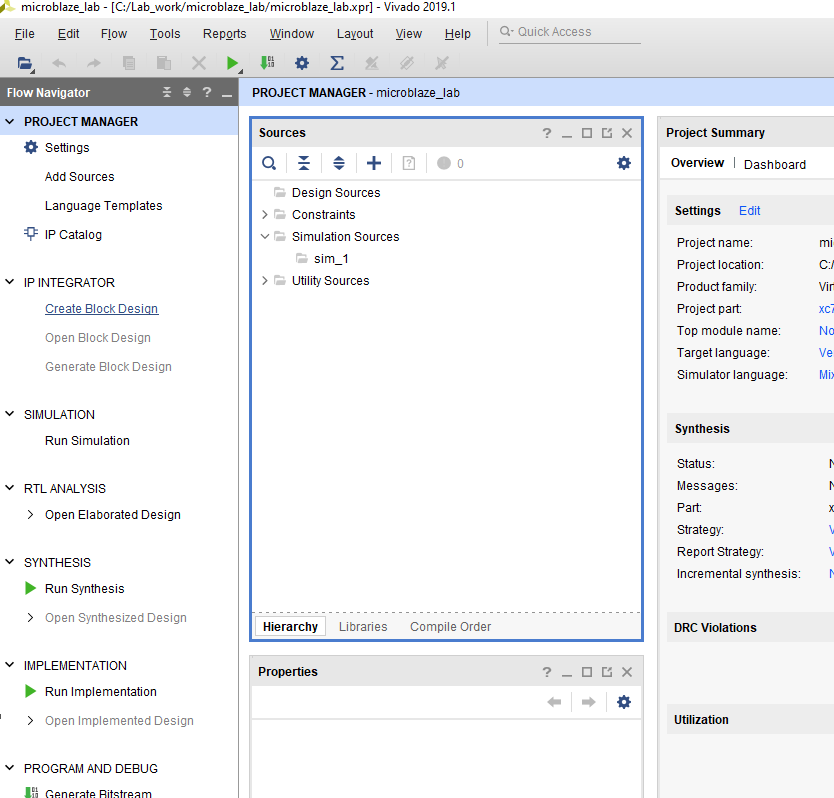
\includegraphics[scale=0.3]{image/m_12.png}   
			\label{m_12}
		\end{minipage}
	}
	\subfigure[Назначаем имя файлу] 
	{
		\begin{minipage}{8cm}
			\centering      
			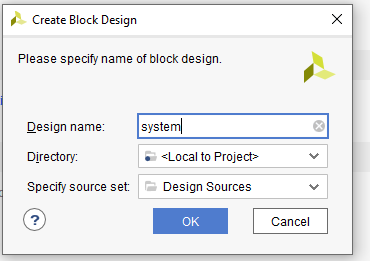
\includegraphics[scale=0.5]{image/m_13.png}   
			\label{m_13}
		\end{minipage}
	}
	\caption{Окно мастера подключения нового файла: кнопка и имя} %  %Имя большого изображения
\end{figure}

После нажатия на кнопку OK Vivado перейдёт в режим \verb|IP Integrator|.

Теперь мы можем начать собирать процессорную систему. Процесс этот во 
многом автоматизирован, и мы этим воспользуемся. Первое, что нам необходимо 
добавить в софт-процессорную систему – это сам софт-процессор MicroBlaze. Есть 
несколько вариантов его исполнения и добавления, но для проектирования таких 
простых систем, как наша, обычно используется мастер настройки. Для добавления 
IP-блоков на схему проекта (вкладка Diagram) можно воспользоваться кнопкой
Add IP или нажать Ctrl+I. После нажатия на кнопку откроется каталог блоков, которые можно 
добавить на поле Diagram.

В появившемся окне со списком доступных IP блоков (рис. ~\ref{m_16}) в поле поиска 
Search пишем MicroBlaze и выбираем из найденных позиций MicroBlaze.

Дважды кликаем по MicroBlaze, после чего IP блок появляется на поле. 
Обратите внимание, что также появилось окно настройки адресов (об этом 
позже), и «свесилась» зелёная строка помощи, которая появляется, если Vivado
может как-то автоматизировать процесс (в нашем случае появилась надпись-ссылка
Run Block Automation) и сам модуль MicroBlaze возник на поле Diagram.

\begin{figure}[!ht]
	\centering
	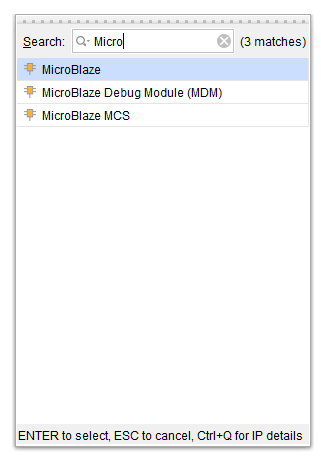
\includegraphics[width=0.3\textwidth]{image/m_16.png}
	\caption{Поиск Microblaze}
	\label{m_16}
\end{figure}

Воспользуемся автоматизацией, нажав на ссылку \verb|Run Block Automation|, после чего появится окно с мастера экспресс настроек процессорной 
системы (рис. ~\ref{m_16}). После вызова мастера доступны именно экспресс-настройки, то 
есть те, которые используются наиболее часто. Расширенные настройки доступны
по двойному щелчку на IP-блоке MicroBlaze, но это выходит за рамки текущей 
статьи.

Из предлагаемых настроек доступны:

\begin{enumerate}
    \item Количество памяти для программы и данных
    \item Управление механизмом коррекции ошибок
    \item Конфигурация кэша
    \item Конфигурация отладчика (тот самый MDM из списка)
    \item Задействование/отключение порта сопряжения с периферией (AXI-порта)
    \item Включение/выключение контроллера прерываний
    \item Выбор сигнала тактирования
\end{enumerate}

Оставим все настройки в значениях по умолчанию и нажмём кнопку OK, т. к. 
для нас этих параметров достаточно. После окончания работы мастера на поле 
появится множество новых блоков, которые мы разберём ниже. 

Как видите, картина изменилась, и на рабочем поле появились:
\begin{enumerate}
	\item Кнопка оптимизации рабочего поля
	\item Предложение по автоматическому подключению одних блоков к другим
(нажмите на неё и посмотрите, что предлагается подключить; после просмотра 
нажмите Отмена – Cancel)
      \item Блок управления тактовой частотой и синхронизацией
	\item Блок сброса процессорной системы
	\item Модуль отладки (отладчик)
	\item Ядро софт-процессора MicroBlaze
	\item Локальная память данных и программ
\end{enumerate}

\begin{figure}[!ht]
	\centering
	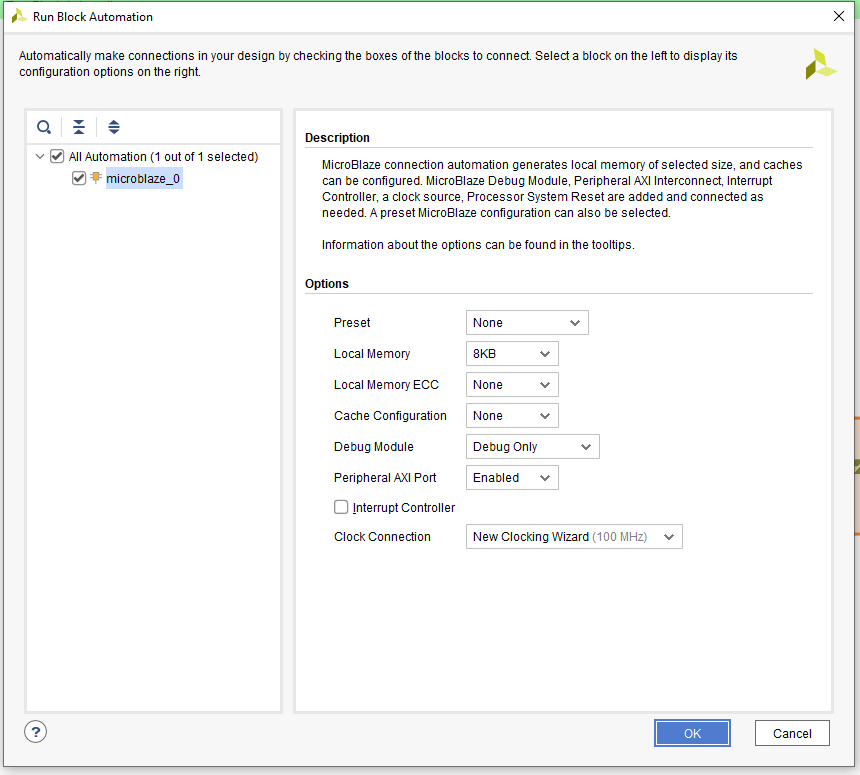
\includegraphics[width=0.4\textwidth]{image/m_18.png}
	\caption{Настройка меню Run Block Automation}
	\label{m_18}
\end{figure}

Теперь добавим необходимую периферию. В начале статьи мы определились, 
что будем мигать светодиодом, и выдавать сообщения по UART. Значит, нужно 
добавить IP-блоки, которые будут обеспечивать этот функционал. Для мигания 
будем использовать IP-блок ввода/вывода общего назначения GPIO, а для вывода сообщений – UART Lite.
Добавление IP блоков аналогично добавлению MicroBlaze. Поэтому нажимаем 
кнопку Add IP, и в поле поиска пишем gpio, выбираем модуль AXI GPIO и нажимаем 
Enter.

После добавления блока AXI GPIO необходимо его настроить, задать 
разрядность портов, определить направление и количество каналов. Настройка 
производится двойным щелчком по блоку либо выбором Customize Block из 
контекстного меню, открывающегося по щелчку правой кнопкой мыши. Модуль
\verb|axi_gpio_0| будет управлять светодиодом, периодически включая и выключая его. 
Значит \verb|axi_gpio_0| должен быть сконфигурирован следующим образом (рис. ~\ref{m_22})

\begin{enumerate}
	\item Задаём направление портов блока AXI GPIO – выбираем, что все выводы 
являются выходами, т. к. мы управляем светодиодом, а не он нами.
	\item Ставим разрядность порта 1 – всего будет подключён 1 светодиод.
	\item Второй канал нам не нужен, отключаем его.
	\item Нажимаем кнопку OK.
\end{enumerate}

Нажав плюсик около интерфейса GPIO модуля \verb|axi_gpio_0| увидим, что порт 
\verb|gpio_io_o| имеет разрядность 1 (вектор [0:0]).

Теперь давайте попробуем подключить наш настроенный блок AXI GPIO к 
MicroBlaze. Предлагаю довериться автоматике и посмотреть, что нам создаст 
Vivado. Нажимаем на строку Run connection Automation и ждём 
появления окна помощника доступных подключений (рис. ~\ref{m_24})

В окне помощника подключений:
\begin{enumerate}
	\item Выберите подключение  \verb|axi_gpio_0| и поставьте галочку \verb|S_AXI| (далее мы 
рассмотрим и поясним это подключение).
	\item Установите подключение тактового сигнала как Auto.
	\item Нажмите OK.
\end{enumerate}

После завершения подключения нажмите кнопку оптимизации рабочего 
пространства в панели инструментов.

\begin{figure}[!ht]
	\centering
	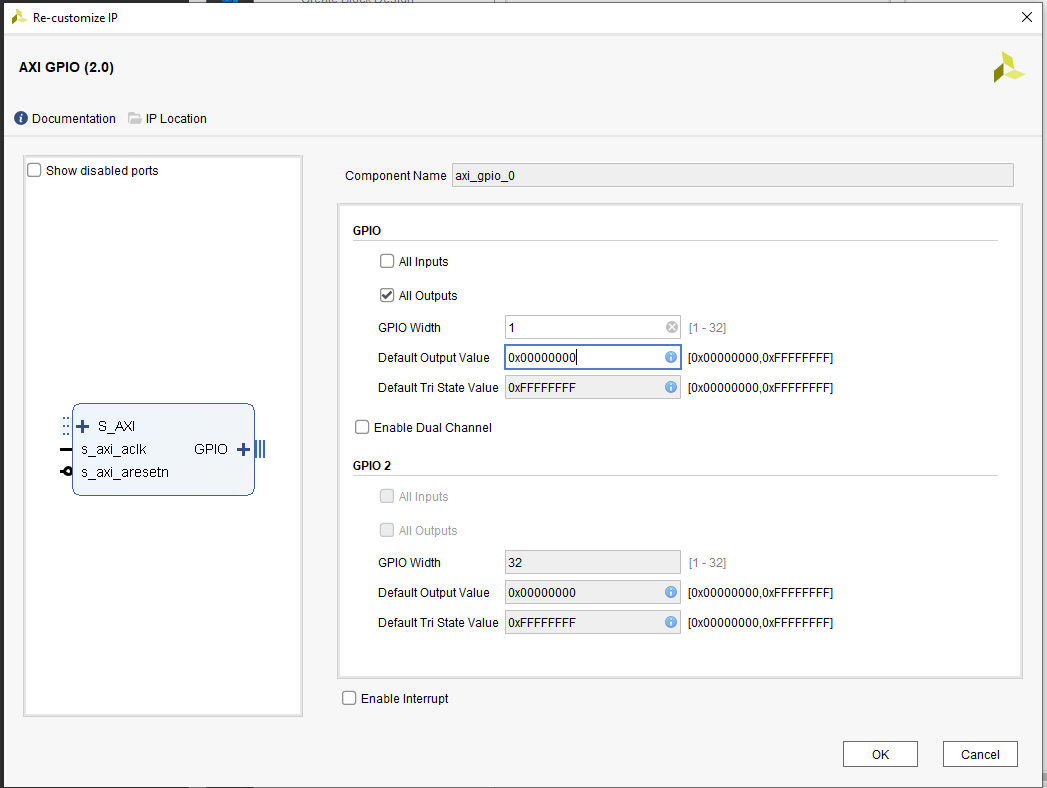
\includegraphics[width=0.4\textwidth]{image/m_22.png}
	\caption{Настройка ядра GPIO}
	\label{m_22}
\end{figure}

Как вы можете заметить, появился дополнительный модуль 
AXI Interconnect. Кратко опишем его назначение. Дело в том, что 
взаимодействие между процессором и периферией происходит по шине AXI. 
На шине есть мастер (обычно это процессор) и слэйв (Slave), в 
нашей литературе это ведущий и ведомый соответственно. Мастер отправляет 
команды слейву. Однако AXI не позволяет подключить к мастеру более одного 
слейва напрямую. Именно напрямую нельзя, но можно через коммутатор, который и 
называется AXI Interconnect – назначение этого модуля обеспечить подключение 
между несколькими мастерами и несколькими слейвами. Пока в нашей системе 
один мастер –  \verb|microblaze_0| и один слейв –  \verb|axi_gpio_0|. 

Теперь давайте попробуем добавить модуль UART Lite в нашу систему.
Надеюсь, что последовательность запомнили. Нажимаем кнопку Add IP, вводим 
в строке поиска Uartlite, дважды кликаем и ждём. 

\begin{figure}[!ht]
	\centering
	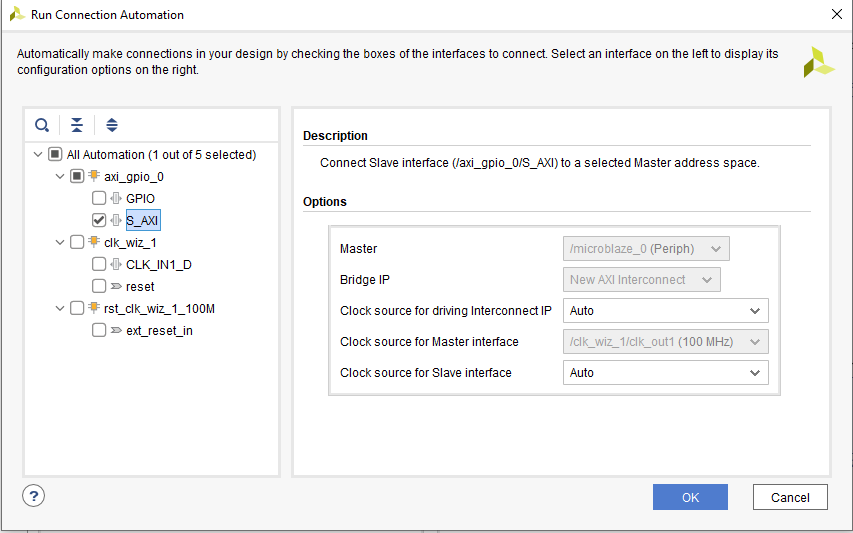
\includegraphics[width=0.4\textwidth]{image/m_24.png}
	\caption{Автоматическое подключение ядра GPIO}
	\label{m_24}
\end{figure}

При желании просмотрите доступные настройки для модуля и если есть 
необходимость, измените. Настройки обычные: скорость (9600), количество стоп
бит (1), чётность (нет), количество бит (8).
Для подключения Uartlite к нашей системе, давайте вновь воспользуемся 
автоматизацией, которую предлагает Vivado, нажав строку Run Connection
Automation. Для модуля  \verb|axi_uart_0| выберите  \verb|S_AXI| и нажмите OK (рис. ~\ref{m_28})

После завершения подключения нажмите кнопку оптимизации рабочего 
пространства и обратите внимание на изменения в AXI
Interconnect. Что произошло и почему? В AXI Interconnect добавился дополнительный 
мастер-порт для подключения второго слэйва (Uartlite – это ведомое устройство). 
MicroBlaze имеет один мастер-порт, который называется  \verb|M_AXI_DP|. Мастер один, 
а слейва два, но подключать напрямую можно только один слейв. Для подключения
нескольких слейвов мы используем AXI Interconnect. Поэтому в AXI Interconnect
добавился ещё один порт. В общем случае, AXI Interconnect может 
обеспечивать взаимное подключение нескольких мастеров и нескольких слейвов.

Теперь давайте настроим модуль управления тактовой 
частотой и синхронизацией  \verb|clk_wiz_1|. 

В окне настроек  \verb|clk_wiz_1|:
\begin{enumerate}
	\item Выберите вкладку Clocking Options.
	\item Тип модуля – MMCM.
	\item Включены возможности синтеза частоты и фазовой подстройки.
	\item Основная тактовая частота – 200MГц.
	\item Тип сигнала с системного тактового генератора на плате –
дифференциальная пара.
	\item На ней – установите выходное значение частоты (тактовая частота 
процессора) – также 100 МГц.
	\item Снимите галочку с сигнала reset.
	\item Установите галочку locked.
	\item Нажмите OK.
\end{enumerate}

Установленные настройки могут повлиять на внешний вид \verb|clk_wiz_1| (для Arty
Board он примет вид, как на рис. 29).

\begin{figure}[!ht]
	\centering
	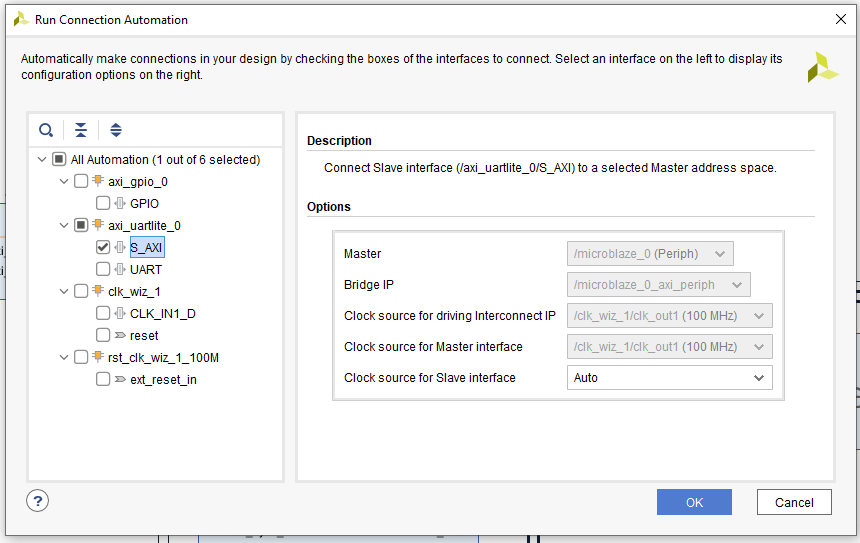
\includegraphics[width=0.7\textwidth]{image/m_28.png}
	\caption{Автоматическое подключение ядра UART}
	\label{m_28}
\end{figure}

Если оставить незадействованные выводы модуля сброса неподключенными, 
то может возникнуть ситуация, при которой процессор будет всегда в состоянии 
сброса. Потому выполним явное их подключение к логического «0» – неактивному 
для них логическому уровню. Для этого(см. рис. ~\ref{m_41}, ~\ref{m_44}):

\begin{enumerate}
	\item Добавьте блок constant.
	\item Установите в нем значение 0 (если по умолчанию оно другое).
	\item Подключите выход блока Constant к входам \verb|aux_reset_in| и  \verb|ext_reset_in|
блока \verb|rst_clk_wiz_1_100M|.
\end{enumerate}

Подключение осуществляется следующим образом: подведите мышку к 
выходу блока Constant (указатель должен принять вид карандашика), нажмите на 
выход и, не отпуская левую кнопку мыши, подведите соединение к входу 
 \verb|aux_reset_in| – а затем повторите те же действия для \verb|ext_reset_in|. В очередной раз 
нажмите кнопку оптимизации рабочего пространства в панели инструментов. 

Теперь необходимо создать внешние входы и выходы для нашей 
процессорной системы. Если вы обратили внимание, сейчас не подключены  \verb|clk_in1| 
и выходы экземпляров модулей \verb|axi_gpio_0| и  \verb|axi_uartlite_0|. Сейчас мы должны 
обозначить, какие порты являются внешними и должны выходить из нашей 
процессорной системы наружу.
Назначим вход \verb|CLK_IN1_D| модуля Clocking Wizard внешним. Для этого кликнем 
по нему правой кнопкой мыши и выберем Create Interface Port.Аналогично поступаем и с выходом GPIO модуля \verb|axi_gpio_0| и шиной UARTмодуля  \verb|axi_uartlite_0| (см. рис. ~\ref{sys_clk},~\ref{m_35},~\ref{m_37} ). 

\begin{figure}[htbp]	
	\subfigure[Тактовый сигнал] 
	{
		\begin{minipage}{8cm}
			\centering         
			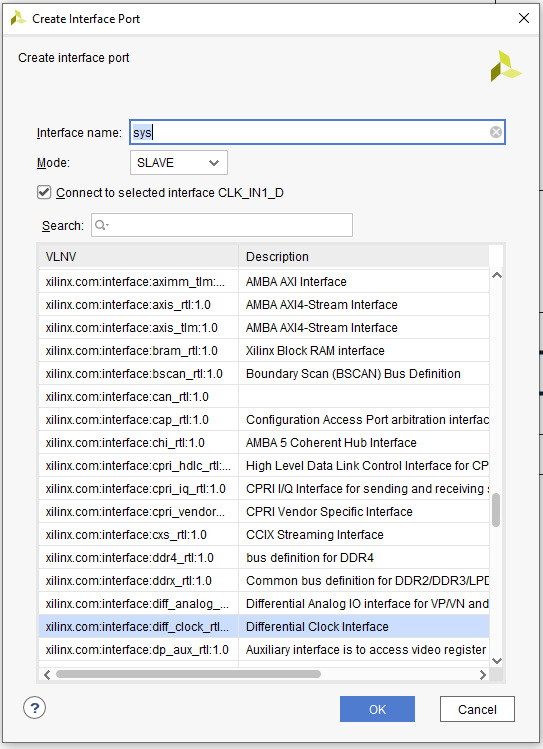
\includegraphics[scale=0.5]{image/gen.PNG}   
			\label{sys_clk}
		\end{minipage}
	}
	\subfigure[GPIO] 
	{
		\begin{minipage}{8cm}
			\centering      
			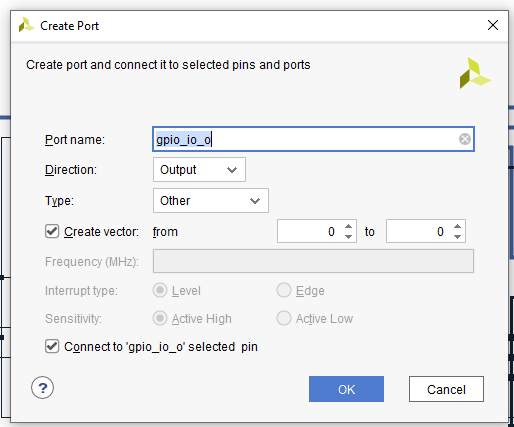
\includegraphics[scale=0.5]{image/m_35.png}   
			\label{m_35}
		\end{minipage}
	}
	\caption{Создание внешнего подключения интерфейсов: тактовый сигнал и GPIO} %  %Имя большого изображения
\end{figure}

\begin{figure}[!ht]
	\centering
	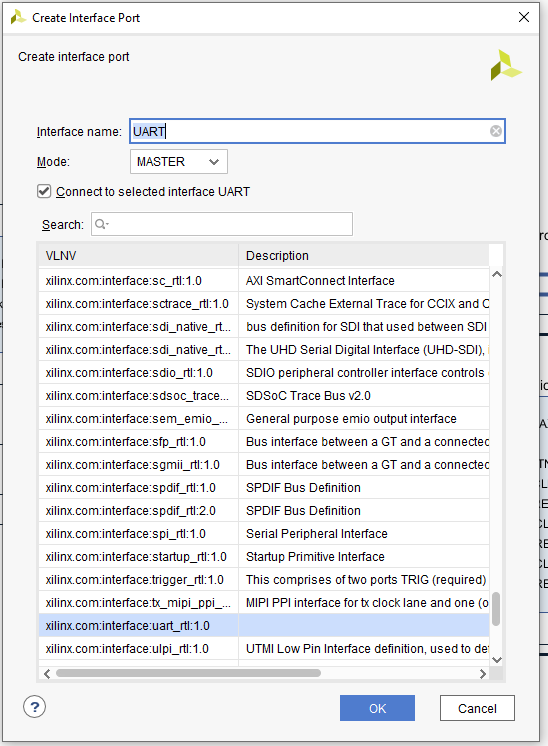
\includegraphics[width=0.3\textwidth]{image/m_37.png}
	\caption{Создание внешнего подключения интерфейса UART}
	\label{m_37}
\end{figure}

\begin{figure}[!ht]
	\centering
	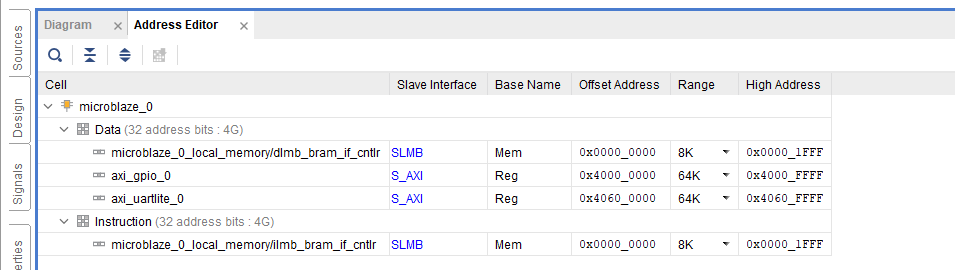
\includegraphics[width=0.8\textwidth]{image/m_39.png}
	\caption{Address Editor}
	\label{Address_Editor}
\end{figure}

Рассмотрим назначение вкладки Address Editor (рис. ~\ref{Address_Editor}).

Наши модули соединены по шине AXI, полное название AXI Memory Map, это 
значит, что все модули, подключённые к шине должны иметь уникальный адрес, 
чтобы процессор смог к ним обратиться и «не перепутать» один модуль с другим. 
Назначение уникальных адресов (распределение адресного пространства) как раз и 
происходит во вкладке \verb|Address Editor|, где в ручном, полуавтоматическом или
автоматическом режиме можно установить диапазон адресов для конкретных 
модулей.

\begin{figure}[!ht]
	\centering
	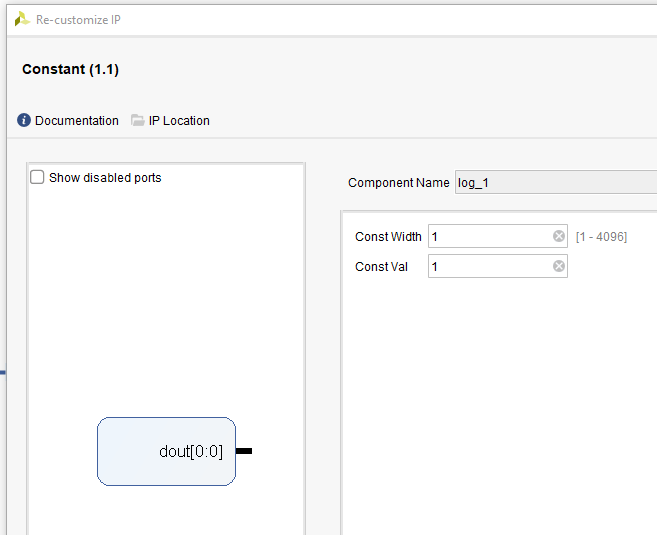
\includegraphics[width=0.4\textwidth]{image/log_1_1.png}
	\caption{Настройка Constant}
	\label{m_41}
\end{figure}

К сожалению, для нашей будущей программы не достаточно памяти, которую 
мы задали, когда пользовались мастером экспресс-настроек MicroBlaze. 
Нам необходимо увеличить количество памяти для данных и инструкций с 8К до 
16К. Сделать это можно простым выбором из выпадающего списка доступного 
количества памяти, нажав на стрелочку в соответствующем поле. Изменить 
необходимо размер памяти и инструкций. В обоих полях должно быть значение 16К.

\begin{figure}[!ht]
	\centering
	\includegraphics[width=0.4\textwidth]{image/log_1.png}
	\caption{Подключение Constant к Processor System Reset}
	\label{m_44}
\end{figure}

\begin{figure}[!ht]
	\centering
	\includegraphics[width=0.4\textwidth]{image/m_46.png}
	\caption{Create HDL Wrapper: первый шаг}
	\label{m_46}
\end{figure}

Мы проделали много действий, закончили собирать систему и назначили все 
адреса. Но все ли корректно и правильно? В панели инструментов на вкладке 
Diagram есть одна из самых важных кнопок, называется она Validate Design. Нажатие этой кнопки запускает инструмент проверки 
ошибок сборки HW части процессорной системы. Нажмите эту кнопку и дождитесь результата. Если же появились ошибки – внимательно прочитайте их и постарайтесь самостоятельно исправить, вернувшись по тексту к соответствующим пунктам либо проделав всю последовательность с начала ещё раз, более внимательно и аккуратно.

\begin{figure}[!ht]
	\centering
	\includegraphics[width=0.4\textwidth]{image/m_47.png}
	\caption{Create HDL Wrapper: второй шаг}
	\label{m_47}
\end{figure}

Нажмите на основной панели Vivado кнопку сохранения, а затем – кнопку 
Project Manager, чтобы выйти из IP Integrator и вернуться в основной режим работы 
Vivado.

Далее следуют стандартные этапы проектирования: синтез, имплементация, 
генерация файла прошивки (битстрима). Но для блочного проекта обязательно 
нужно сделать обёртку (wrapper); это показано на рис. ~\ref{m_46},~\ref{m_47}. Нажмите правой кнопкой на созданном блочном проекте и выберите Create HDL Wrapper. В появившемся 
окне нажмите OK.

\begin{Verbatim}[tabsize=4]
# SYSCLK 200MHz
set_property PACKAGE_PIN E19 [get_ports sys_clk_p]
set_property IOSTANDARD LVDS [get_ports sys_clk_p]
set_property PACKAGE_PIN E18 [get_ports sys_clk_n]
set_property IOSTANDARD LVDS [get_ports sys_clk_n]

# LED_0
set_property PACKAGE_PIN AM39 [get_ports gpio_io_o]
set_property IOSTANDARD LVCMOS18 [get_ports gpio_io_o]

# UART
set_property PACKAGE_PIN AU33 [get_ports UART_rxd]
set_property IOSTANDARD LVCMOS18 [get_ports UART_rxd]
set_property PACKAGE_PIN AU36 [get_ports UART_txd]
set_property IOSTANDARD LVCMOS18 [get_ports UART_txd]

\end{Verbatim}

Обёртка – это простой VHDL- или Verilog-файл (с расширениями «vhd» или 
«v» соответственно), в который включена наша процессорная система, как часть 
иерархии. Таким образом, нашей собранной процессорной системой мы сможем 
оперировать, как простым модулем, добавляя её в качестве подмодуля в модули 
верхнего уровня. После создания обёртки наш модуль можно наконец-то запустить 
на синтез, нажав на кнопу Run Synthesis.

Окно, появляющееся после синтеза, предлагает выполнить:
\begin{enumerate}
	\item Запустить имплементацию.
	\item Открыть синтезируемый проект (Выберите этот пункт).
	\item Просмотреть отчёты.
\end{enumerate}
Нажмите Generate Bitstream и затем, когда Vivado предложит выполнить 
синтез и имплементацию перед запуском генерации bit-файла – нажмите Yes.
Теперь нам нужно ждать окончания генерации bit-файла. Это может занять 
минут 10-15 в зависимости от Вашего компьютера. 
По окончании генерации bit файла появится окно (рис. 50), предлагающее выполнить одно из действий. Нам 
ничего дальше делать не нужно, поэтому его просто закрываем.

\section{Проект в Xilinx SDK}

SW-часть (программная) необходима, чтобы «оживить» нашу собранную 
процессорную систему. Сейчас это просто кусок «железа», который не выполняет 
никаких действий. Как уже было сказано выше, разработка программной части 
выполнятся в среде Xilinx SDK, которая есть по сути Eclipse с плагинами от Xilinx. 
Разумеется, что Xilinx уже автоматизировал часть процесса написания программы и 
подготовил некоторые исходные файлы и библиотеки, так что писать мы будем не 
«с нуля». Сейчас нам необходимо передать Xilinx SDK информацию об аппаратной 
«начинке» нашей процессорной системы: какие использованы устройства, какова их 
конфигурация и адреса и т.д. В общем – выполнить экспорт нашей аппаратной (HW) 
части. Сделать это можно, выбрав в левом верхнем углу File -> Export -> Export Hardware
(рис. ~\ref{hw_1})

\begin{figure}[htbp]	
	\subfigure[Экспорт HW-части проекта в Xilinx SDK] 
	{
		\begin{minipage}{8cm}
			\centering         
			\includegraphics[scale=0.5]{image/hw_1.png}   
			\label{hw_1}
		\end{minipage}
	}
	\subfigure[Параметры экспорта HW части] 
	{
		\begin{minipage}{8cm}
			\centering      
			\includegraphics[scale=0.5]{image/hw_2.png}   
			\label{hw_2}
		\end{minipage}
	}
	\caption{Экспорт HW-части проекта в Xilinx SDK} %  %Имя большого изображения
\end{figure}


После этого появится окно (рис. ~\ref{hw_2}), в котором указывается, нужно ли 
экспортировать bit-файл, и какую папку выбрать в качестве рабочей. Оставим все 
настройки в состояниях по умолчанию; bit-файл экспортировать сейчас не надо, мы 
добавим его позже. Нажимаем OK.


\begin{figure}[htbp]	
	\subfigure[Назначаем проекту имя] 
	{
		\begin{minipage}{8cm}
			\centering         
			\includegraphics[scale=0.3]{image/image61.png}   
			\label{image61}
		\end{minipage}
	}
	\subfigure[Настраиваем параметры проекта] 
	{
		\begin{minipage}{8cm}
			\centering      
			\includegraphics[scale=0.5]{image/image62.png}   
			\label{image62}
		\end{minipage}
	}
	\caption{Создание нового проекта в Xilinx SDK} %  %Имя большого изображения
\end{figure}

Теперь запускаем программу Xilinx SDK. Сделать это можно через главное 
меню Windows или из-под Vivado – просто выберите в левом верхнем углу File->Launch SDK.

Теперь Vivado просит указать параметры запуска SDK; отставим их по 
умолчанию и нажмём OK.

Приступим к созданию проекта. Выбираем File-New-Application project
Задаём основные параметры проекта (рис. ~\ref{image62}):

\begin{enumerate}
	\item Название проекта.
	\item Место расположения проекта (выставляем используемое по 
умолчанию).
	\item Тип используемой в проекте операционной системы (без ОС –
standalone).
	\item Аппаратная конфигурация (если процессоров системе несколько, то 
будет список; у нас – только один).
	\item Идентификатор процессора (актуально для многопроцессорных систем).
	\item Язык программирования (чистый C).
	\item Пакет драйверов (создаём новый на основании информации о HW части).
	\item Нажимаем Next.
\end{enumerate}

Теперь SDK предлагает выбрать один из нескольких готовых вариантов 
приложения, выбираем Hello world. После нажатия на кнопку Finish в 
проект добавляется несколько файлов и папок.

\begin{figure}[!ht]
	\centering
	\includegraphics[width=0.5\textwidth]{image/SDK_Exp.png}
	\caption{Project Explorer в Xilinx SDK}
	\label{SDK_Exp}
\end{figure}

Откройте файл helloworld.c(см. рис. ~\ref{SDK_Exp}) и заполните его следующим кодом:

\begin{Verbatim}[tabsize=4]
#include <stdio.h>
#include "platform.h"
#include "xil_printf.h"

#include "xgpio.h"

XGpio gpio;

int main()
{
    init_platform();

    xil_printf("Hello World\n\r");

    u32 i = 0;
    u32 led = 0;
    XGpio_Initialize(&gpio, XPAR_GPIO_0_DEVICE_ID);

    while(1)
    {
    	i++;
    	if(i == 1000000)
    	{
    		led = !led;
    		XGpio_DiscreteWrite(&gpio, 1, led);
       		i = 0;
    	}
    }

    cleanup_platform();
    return 0;
}
\end{Verbatim}

После этого нажмите кнопку Build на верхней панели. 

\begin{figure}[htbp]	
	\subfigure[Настройка->COM-порт...] 
	{
		\begin{minipage}{8cm}
			\centering         
			\includegraphics[scale=0.5]{image/Terra_0.png}   
			\label{terra_wind}
		\end{minipage}
	}
	\subfigure[Terra Term: Serial Port and Setup Connection] 
	{
		\begin{minipage}{8cm}
			\centering      
			\includegraphics[scale=0.5]{image/terra.png}   
			\label{terra_com}
		\end{minipage}
	}
	\caption{Настройка программы Terra Term} %  %Имя большого изображения
\end{figure}

Перед тем как прошивать ПЛИС настроим Terra Term для просмотра сообщений переданных по UART от софт-процессора(см. рис. ~\ref{terra_wind}, ~\ref{terra_com}).
После успешной сборки проекта и настройки Terra Term можно прошивать ПЛИС. Для этого нажмите Program FPGA(см. рис. ~\ref{program_FPGA}).

\begin{figure}[!ht]
	\centering
	\includegraphics[width=0.5\textwidth]{image/program_FPGA.png}
	\caption{Program FPGA в Xilinx SDK}
	\label{program_FPGA}
\end{figure}

В результате прошивки ПЛИС нулевой светодиод на плате VC707 должен начать мигать, а в Terra Term должно появиться сообщение «Hello, world!»(см. рис. ~\ref{terra_result}).

\begin{figure}[!ht]
	\centering
	\includegraphics[width=0.5\textwidth]{image/terra_result.png}
	\caption{Результаты вывода сообщения в консоль}
	\label{terra_result}
\end{figure}

\newpage

Задачи:

\begin{enumerate}
	\item Сделайте бегущие огни из восьми светодиодов, которые установлены на отладочной плате VC707.
	\item Настройте ядро GPIO таким образом, что бы можно было считывать состояния кнопок, установленных на плате, и отображать их состояние в Terra Term.
\end{enumerate}

Вопросы:

\begin{enumerate}
	\item Как работает ядро Processor System Reset? В какой последовательности и с какими задержками оно формирует сброс?
	\item Какой формат пакета имеет интерфейс UART?
	\item Какие регистры есть у ядра AXI UARTLite? Нарисуйте структурную схему данного ядра.
\end{enumerate}

\chapter{Лабораторная работа №5. Создание IP ядра с управлением по AXI4-Lite}

\section{Интерфейс AXI4-Lite}

Интерфейс AXI4-Lite состоит из следующих независимых каналов транзакций:

\begin{itemize}
	\item Read Address Channel, кратко AR
	\item Write Address Channel, кратко AW
	\item Read Data Channel, кратко R
	\item Write Data Channel, кратко W  
	\item Write Response Channel, кратко B
\end{itemize}

На рисунках~\ref{AXI_read_channel} и~\ref{AXI_write_ch} представлена архитектура каналов AXI4-Lite, а в таблицах ~\ref{WA} - ~\ref{WRC} представлено описание всех пяти каналов интерфейса AXI4.

Read Address Channel предназначен для передачи управляющей информации и адреса чтения от ведущего(master) к ведомому(slave) для совершения транзакции чтения. Read Data Channel предназначен для передачи данных от ведомого к ведущему. Транзакция чтения происходит следующим образом: ведущий передаёт управляющую информацию и адрес чтения ведомому на канале AR, если тот принял её, то он формирует ответ на канале R c запрошенными данными.

Write Address Channel предназначен для передачи управляющей информации от ведущего к ведомому для совершения транзакции записи.Write Data Channel предназначен для передачи данных от ведущего к ведомому при записи данных. Write Response Channel предназначен для формирования ответа ведомым о состоянии транзакции записи. Транзакция записи происходит следующим образом: ведущий передаёт управляющую информацию и адрес записи ведомому на канале AW, если тот принял её, то на канале W ведущий формирует транзакцию записи, после этого ожидаем ответ на канале B. 

\begin{figure}[htbp]	
	\subfigure[Архитектура канала чтения интерфейса AXI] 
	{
		\begin{minipage}{8cm}
			\centering         
			\includegraphics[scale=0.4]{image/AXI_read_ch.png}   
			\label{AXI_read_channel}
		\end{minipage}
	}
	\subfigure[Архитектура канала записи интерфейса AXI] 
	{
		\begin{minipage}{8cm}
			\centering      
			\includegraphics[scale=0.4]{image/AXI_write_ch.png}   
			\label{AXI_write_ch}
		\end{minipage}
	}
	\caption{Архитектура каналов чтения и записи в AXI} %  %Имя большого изображения
\end{figure}

\renewcommand{\arraystretch}{1.1} %% increase table row spacing

\begin{table}[!ht]
	\centering
	\caption{Cигналы Write Address Channel AXI4-Lite}
	\label{WA}
	\begin{tabular}{c c p{0.6\textwidth}} 
		\toprule
		Сигнал & Источник & Описание \\ 
		\midrule
		AWADDR & Master & Адрес записи. Адрес записи дает адрес 
		первой передачи при пакетной транзакции. \\
		AWVALID & Master  & \multirow{2}{*}{Сигналы механизма "рукопожатий".} \\ 
		AWREADY & Slave  &   \\
		\bottomrule
	\end{tabular}
\end{table}

\begin{table}[!ht]
		\centering
		\caption{Описание сигналов Read Address Channel интерфейса AXI4-Lite}
		\label{RA}
		\begin{tabular}{ c  c  p{0.6\textwidth} } 
			\toprule
			Сигнал & Источник & Описание \\ 
			\midrule 
			ARADDR & Master & Адрес по которому будет происходит операция чтения данных. Для пакетной транзакции дает адрес первой операции чтения.\\
			ARVALID & Master  & \multirow{2}{*}{Сигналы механизма "рукопожатий".} \\ 
			ARREADY & Slave  & \\
			\bottomrule
		\end{tabular}
\end{table}

\begin{table}[!ht]
	\centering
	\caption{Сигналы Write Data Channel AXI4-Lite}
	\label{WD}
	\begin{tabular}{ c  c  p{0.6\textwidth} } 
		\toprule
		Сигнал & Источник & Описание \\ 
		\midrule
		WDATA & Master & Шина данных записи. \\ 
		WSTRB & Master  & Cтробы данных записи. Этот сигнал указывает, какие байты содержат действительные данные. На каждые восемь бит шины данных записи приходится один стробирующий бит записи. \\ 
		WVALID & Slave  & \multirow{2}{*}{Сигналы механизма "рукопожатий".} \\ 
		WREADY & Slave  & \\
		\bottomrule
	\end{tabular}

\end{table}

\begin{table}[!ht]
	\centering
	\caption{Сигналы Read Data Channel AXI4-Lite}
	\label{RD}
		\begin{tabular}{  c c  p{0.6\textwidth} } 
			\toprule
			Сигнал & Источник & Описание \\ 
			\midrule
			RDATA & Slave & Прочитанные данные. \\ 
			RRESP & Slave  & Этот сигнал указывает на состояние транзакции чтения. \\ 
			RVALID & Slave  & \multirow{2}{*}{Сигналы механизма "рукопожатий".} \\ 
			RREADY & Master  & \\ 
			\bottomrule
		\end{tabular}
\end{table}

\begin{table}[!ht]
	\centering
	\caption{Сигналы Write Response Channel AXI4-Lite}
	\label{WRC}
		\begin{tabular}{  c c  p{0.6\textwidth} } 
			\toprule
			Сигнал & Источник & Описание \\
			\midrule
			BRESP & Slave  & Ответ на запись. Этот сигнал указывает на состояние транзакции записи. \\
			BVALID & Slave  & \multirow{2}{*}{Сигналы механизма "рукопожатий".} \\ 
			BREADY & Master  & \\ 
			\bottomrule
		\end{tabular}
\end{table}

\clearpage

Рассмотрим механизм обмена данными в AXI4. Все пять каналов транзакций используют один и тот же процесс подтверждения VALID/READY для передачи адреса, данных и управляющей информации. Этот двусторонний механизм управления потоком означает, что и ведущий, и ведомый могут управлять скоростью, с которой информация перемещается между ведущим и ведомым. Источник генерирует сигнал VALID, чтобы указать, когда адрес, данные или управляющая информация доступны. Приёмник генерирует сигнал READY, чтобы указать, что он может принять информацию. Передача происходит только тогда, когда оба сигнала VALID и READY имеют высокий уровень.

\begin{figure}[!ht]
	\centering
	\includegraphics[width=0.4\textwidth]{image/AXI-handshape}
	\caption{Механизм обмена данными - VALID до READY}
	\label{AXI-valid_before_ready}
\end{figure}

На рисунке~\ref{AXI-valid_before_ready} источник представляет адрес, данные или управляющую информацию после T1 и утверждает сигнал VALID. Приёмник устанавливает сигнал READY после T2, а источник должен сохранять свою информацию стабильной до тех пор, пока передача не произойдет в T3.


\begin{figure}[!ht]
	\centering
	\includegraphics[width=0.4\textwidth]{image/AXI-hand-valid}
	\caption{Механизм обмена данными - READY и VALID одновременно}
	\label{AXI-valid_ready}
\end{figure}


На рисунке~\ref{AXI-valid_ready} и источник, и приёмник после T1 указывают, что они могут передавать/принимать адрес, данные или управляющую информацию. В этом случае передача происходит по нарастающему фронту тактового сигнала T2, когда как VALID, так и READY имеют высокий уровень напряжения.

\begin{figure}[!ht]
	\centering
	\includegraphics[width=0.4\textwidth]{image/AXI-hand_ready}
	\caption{Механизм обмена данными - READY до VALID}
	\label{AXI-handshape}
\end{figure}

На рисунке~\ref{AXI-handshape} приёмник утверждает READY после T1, прежде чем адрес, данные или управляющая информация являются действительными, указывая на то, что он может принять информацию. Источник представляет информацию и утверждает VALID после T2, и передача происходит в T3.

\section{Транзакции чтения и записи интерфейса AXI4-Lite}

На рисунке ~\ref{AXI_wr_tr} представлен пример транзакции записи интерфейса AXI4-Lite.
Опишем последовательность выполнения транзакции.

\begin{figure}[h]
	\centering
	\includegraphics[width=0.8\textwidth]{image/axi_lite_write}
	\caption{AXI4-Lite транзакция записи}
	\label{AXI_wr_tr}
\end{figure}

\begin{enumerate}
	\item Мастер помещает адрес в канал адреса записи, а данные - в канал данных записи. В то же время он утверждает AWVALID и WVALID, указывая, что адрес и данные на соответствующих каналах действительны. BREADY также утверждается Мастером, указывая на то, что он готов получить ответ.
	\item Подчиненное устройство устанавливает AWREADY и WREADY на каналы адреса записи и записи данных соответственно.
	\item Поскольку сигналы «Действительный» и «Готово» присутствуют как на каналах адреса записи, так и на каналах записи данных, на этих каналах происходит подтверждение связи, и соответствующие сигналы «Действительный» и «Готово» могут быть отменены. (После того, как произойдут оба рукопожатия, ведомое устройство имеет адрес записи и данные)
	\item Подчиненное устройство заявляет BVALID, указывая на наличие действительного ответа по каналу ответа на запись. (в данном случае ответ 2'b00, это «ОК»).
	\item Следующий нарастающий фронт тактовой частоты завершает транзакцию, при этом сигналы Ready и Valid в канале ответа на запись имеют высокий уровень.
\end{enumerate}

На рисунке ~\ref{AXI_wr_tr} представлен пример транзакции чтения интерфейса AXI4-Lite.
Опишем последовательность выполнения транзакции.

\begin{figure}[h]
	\centering
	\includegraphics[width=0.8\textwidth]{image/axi_lite_read}
	\caption{AXI4-Lite транзакция чтения}
	\label{AXI_rd_tr}
\end{figure}

\begin{enumerate}
	\item Мастер помещает адрес в канал адреса чтения, а также устанавливает ARVALID, указывая, что адрес действителен, и RREADY, указывая, что мастер готов принять данные от подчиненного устройства.
	\item Подчиненный заявляет ARREADY, указывая, что он готов принять адрес на шине.
	\item Поскольку подтверждены как ARVALID, так и ARREADY, на следующем нарастающем фронте тактового сигнала происходит квитирование, после чего ведущее и ведомое устройства отменяют ARVALID и ARREADY, соответственно. (На этом этапе ведомое устройство получило запрошенный адрес).
	\item Подчиненное устройство помещает запрошенные данные в канал чтения данных и устанавливает RVALID, указывая, что данные в канале действительны. Подчиненное устройство также может отправить ответ на RRESP, хотя здесь этого не происходит.
	\item Поскольку подтверждены и RREADY, и RVALID, следующий нарастающий фронт тактовой частоты завершает транзакцию. RREADY и RVALID теперь можно отключить.
\end{enumerate}

Подтверждения связи в канале адреса записи и записи данных не обязательно происходят одновременно (как в показанной транзакции). Однако спецификация AXI4 утверждает, что оба должны произойти, прежде чем ведомое устройство сможет отправить ответ на запись. Подтверждение адреса записи и записи данных может происходить независимо или одновременно, и никакой порядок не применяется, только оба должны произойти для завершения транзакции.

\section{AXI4-Lite и конфигурационные регистры ядра}

У ядра предусмотрен(если нужно) набор конфигурационных регистров. Чаще всего регистры сгруппированы по словам (например, 32-битным), где внутри разделяются по полям(в пределах одного регистра могут быть несколько полей), у которых могут быть различные режимы работы:
\begin{enumerate}
	\item RW — read and write: можно писать и читать. Служат для настройки ядра (например, включение того или иного режима работы, настройка каких-то параметров и пр.).
	\item RW/SC — read write self clear: если записать единицу, то она сама сбросит в ноль (может быть удобно для ресета ядра или модуля ядра: ставишь единицу, а он сам сбросит себя в ноль).
	\item RO — read only: только читать (например, для статистики или о состояния ядра). Так же некоторые регистры делаются RO для хранения константных значений (например, версию ядра, либо его возможности).
\end{enumerate}

Конфигурационные регистры так же есть у различных микросхем, таких как аналого-цифровые и цифро-аналоговые преобразователи, системы фазовой автоподстройки частоты, микросхемы реализующие физический уровень интерфейса Ethernet и у многих других.

При проектирование цифровых устройств на ПЛИС фирмы Xilinx конфигурационные регистры ядра чаще всего реализуются с использованием интерфейса AXI4-Lite. Среда разработки Vivado Design Suite при создании проекта IP ядра позволяет получить код ведомого(slave) интерфейса AXI4-Lite, который можно легко использовать для создания системы конфигурационных регистров ядра. Укажем, что кроме этого генерировать можно ведущий(master) интерфейс AXI4-Lite, а также ведущий(master) и ведомый(slave) таких интерфейсов как AXI4 и AXI4-Stream.

\section{Создание IP ядра в Vivado}

Для создания собственного IP ядра в Vivado нажмите \verb|Tools -> Create and Package New Ip...|(см. рис. ~\ref{create_and_pkg_new_ip_0}, ~\ref{create_and_pkg_new_ip_1}).
Во вкладке \verb|Create Peripheral, Package IP or Package a Block Deisgn| выбираем пункт создания ядра с AXI4 интерфейсом: \verb|Create a new AXI4 peripheral|(см. рис. ~\ref{create_and_pkg_new_ip_2}). В следующей вкладке \verb|Peripheral Details| введите имя, версию, описание и путь до ядра как показано на~\ref{create_and_pkg_new_ip_3}.

\begin{figure}[htbp]	
	\subfigure[Tools->Create and Package New Ip...] 
	{
		\begin{minipage}{8cm}
			\centering         
			\includegraphics[scale=0.5]{image/create_and_pkg_new_ip_0.png}   
			\label{create_and_pkg_new_ip_0}
		\end{minipage}
	}
	\subfigure[Окно мастера создания IP ядра] 
	{
		\begin{minipage}{8cm}
			\centering      
			\includegraphics[scale=0.3]{image/create_and_pkg_new_ip_1.png}   
			\label{create_and_pkg_new_ip_1}
		\end{minipage}
	}
	\caption{Запуск мастера создания IP ядра} %  %Имя большого изображения
\end{figure}


\begin{figure}[htbp]	
	\subfigure[Create a new AXI4 peripheral] 
	{
		\begin{minipage}{8cm}
			\centering         
			\includegraphics[scale=0.3]{image/create_and_pkg_new_ip_2.png}   
			\label{create_and_pkg_new_ip_2}
		\end{minipage}
	}
	\subfigure[Создаём параметры нового IP ядра] 
	{
		\begin{minipage}{8cm}
			\centering      
			\includegraphics[scale=0.3]{image/create_and_pkg_new_ip_3.png}   
			\label{create_and_pkg_new_ip_3}
		\end{minipage}
	}
	\caption{Тип и параметры ядра} %  %Имя большого изображения
\end{figure}

\begin{figure}[htbp]	
	\subfigure[Выбор интерфейса] 
	{
		\begin{minipage}{8cm}
			\centering         
			\includegraphics[scale=0.3]{image/create_and_pkg_new_ip_4.png}   
			\label{create_and_pkg_new_ip_4}
		\end{minipage}
	}
	\subfigure[Выбор следующий шага после генерации ядра] 
	{
		\begin{minipage}{8cm}
			\centering      
			\includegraphics[scale=0.3]{image/create_and_pkg_new_ip_5.png}   
			\label{create_and_pkg_new_ip_5}
		\end{minipage}
	}
	\caption{Выбор интерфейса и следующего шага после генерации ядра} %  %Имя большого изображения
\end{figure}

\begin{Verbatim}[tabsize=4]
module lcd #(
	parameter CYCLES_PER_US = 50
)
(
	input wire clk,    
	input wire rst, 
	output wire [2:0] ctrl_lcd,
	output wire [3:0] data_lcd,

	output wire 		lcd_ready,
 	input wire 			lcd_valid,
 	input wire [31:0] 	lcd_data_str_0_0,
 	input wire [31:0] 	lcd_data_str_0_1,
 	input wire [31:0] 	lcd_data_str_0_2,
 	input wire [31:0] 	lcd_data_str_0_3,
 	input wire [31:0] 	lcd_data_str_1_0,
 	input wire [31:0] 	lcd_data_str_1_1,
 	input wire [31:0] 	lcd_data_str_1_2,
 	input wire [31:0] 	lcd_data_str_1_3
);

	localparam [3:0]
		WAITING = 4'd0,
        INIT_H30_ONE = 4'd1,
        INIT_H30_TWO = 4'd2,
        INIT_H30_THREE = 4'd3,
        INIT_H20 = 4'd4,
        INIT_FUNCTION_SET = 4'd5,
        INIT_DISPLAY_ON = 4'd6,
		INIT_DISPLAY_CLEAR = 4'd7,
		INIT_SET_ENTRY_MODE = 4'd8,
		CUR_FIRST_ROW = 4'd9,
		WRITE_UPPER_LINE = 4'd10,
		COUNTER_UPPER_LINE = 4'd11,
		CUR_SECOND_ROW = 4'd12,
		WRITE_LOWER_LINE = 4'd13,
		COUNTER_LOWER_LINE = 4'd14,
		LCD_WAIT_VALID = 4'd15;

	reg lcd_ready_r;

	assign lcd_ready = lcd_ready_r;

\end{Verbatim}

\begin{Verbatim}[tabsize=4]
               	LCD_WAIT_VALID: begin
               		if(lcd_valid) begin
               			lcd_ready_r <= 1'b0;
               			lcd_state_r <= CUR_FIRST_ROW;
               			upper_line[0] <= lcd_data_str_0_0[7:0]; 
						upper_line[1] <= lcd_data_str_0_0[15:8]; 
						upper_line[2] <= lcd_data_str_0_0[23:16];
						upper_line[3] <= lcd_data_str_0_0[31:24];
						upper_line[4] <= lcd_data_str_0_1[7:0]; 
						upper_line[5] <= lcd_data_str_0_1[15:8]; 
						upper_line[6] <= lcd_data_str_0_1[23:16]; 
						upper_line[7] <= lcd_data_str_0_1[31:24]; 
						upper_line[8] <=  lcd_data_str_0_2[7:0];  
						upper_line[9] <=  lcd_data_str_0_2[15:8]; 
						upper_line[10] <= lcd_data_str_0_2[23:16]; 
						upper_line[11] <= lcd_data_str_0_2[31:24]; 
						upper_line[12] <= lcd_data_str_0_3[7:0]; 
						upper_line[13] <= lcd_data_str_0_3[15:8]; 
						upper_line[14] <= lcd_data_str_0_3[23:16]; 
						upper_line[15] <= lcd_data_str_0_3[31:24]; 

               			lower_line[0] <= lcd_data_str_1_0[7:0]; 
						lower_line[1] <= lcd_data_str_1_0[15:8];
						lower_line[2] <= lcd_data_str_1_0[23:16]; 
						lower_line[3] <= lcd_data_str_1_0[31:24]; 
						lower_line[4] <= lcd_data_str_1_1[7:0]; 
						lower_line[5] <= lcd_data_str_1_1[15:8];
						lower_line[6] <= lcd_data_str_1_1[23:16]; 
						lower_line[7] <= lcd_data_str_1_1[31:24];
						lower_line[8] <=  lcd_data_str_1_2[7:0];
						lower_line[9] <=  lcd_data_str_1_2[15:8]; 
						lower_line[10] <= lcd_data_str_1_2[23:16];
						lower_line[11] <= lcd_data_str_1_2[31:24];
						lower_line[12] <= lcd_data_str_1_3[7:0]; 
						lower_line[13] <= lcd_data_str_1_3[15:8]; 
						lower_line[14] <= lcd_data_str_1_3[23:16]; 
						lower_line[15] <= lcd_data_str_1_3[31:24]; 
               		end else begin
               			lcd_ready_r <= 1'b1;
						lcd_state_r <= LCD_WAIT_VALID;
               		end
               	end
\end{Verbatim}

\begin{Verbatim}[tabsize=4]
				COUNTER_LOWER_LINE: begin
               		if(counter_lower_line_r == 32'd15) begin
						counter_lower_line_r <= 32'b0;
						lcd_state_r <= LCD_WAIT_VALID;		
                	end else begin
	                	counter_lower_line_r <= counter_lower_line_r + 1;
	                	lcd_state_r <= WRITE_LOWER_LINE;
                	end
               	end
\end{Verbatim}
\section{Верификация ядра с интерфейсом AXI4-Lite}
Если мы разрабатываем ядро, реализуя конфигурационные регистры с использованием ведомого интерфейса AXI4-Lite, то при тестировании ядра необходимо в соответствии с логикой работы ядра заполнить конфигурационные регистры. Для этого необходимо написать тестбенч для ведущего(мастера) интерфейса AXI4-Lite.

\begin{Verbatim}[tabsize=4]
`timescale 1ns/1ps

module tb_lcd();
	
	parameter integer AXI_DATA_WIDTH = 32;
	parameter integer AXI_ADDR_WIDTH = 6;
	parameter integer T_SYS_CLK = 5;


	parameter integer ADDR_DATA_STR_0_0 = 0;
	parameter integer ADDR_DATA_STR_0_1 = 4;
	parameter integer ADDR_DATA_STR_0_2 = 8;
	parameter integer ADDR_DATA_STR_0_3 = 12;
	parameter integer ADDR_DATA_STR_1_0 = 16;
	parameter integer ADDR_DATA_STR_1_1 = 20;
	parameter integer ADDR_DATA_STR_1_2 = 24;
	parameter integer ADDR_DATA_STR_1_3 = 28;
	parameter integer ADDR_VALID 		= 36;


	reg [AXI_ADDR_WIDTH - 1:0] 	axil_awaddr;
	reg 						axil_awvalid;
	wire 						axil_awready;
	
	reg [AXI_DATA_WIDTH - 1:0] 	axil_wdata;
	wire 						axil_wready;
	reg 	 					axil_wvalid;
	
	reg 	 					axil_bready;
	wire 						axil_bvalid;

	reg [AXI_ADDR_WIDTH - 1:0] 	axil_araddr;
	reg 						axil_arvalid;
	wire 						axil_arready;
	
	wire [AXI_DATA_WIDTH - 1:0] axil_rdata;
	reg 						axil_rready;
	wire 						axil_rvalid;

	reg [7:0] upper_line [15:0];
	reg [7:0] lower_line [15:0];

	reg sys_clk;
	reg sys_rst;

	initial 
		sys_clk = 1'b0;
	always 
		sys_clk = #(T_SYS_CLK/2) ~sys_clk;

	task delayT_t;
		input [31:0] T;
		input [31:0] N;
		begin
			repeat (N)
			#T;
		end
	endtask
	
	task AXI4_Lite_W;
		input [31:0] T;
		input [31:0] ADDR;
		input [31:0] DATA;
		begin
			delayT_t(T,2);
			axil_awaddr <= ADDR;
			axil_awvalid <= 1;
			axil_wdata <= DATA;
			axil_wvalid <= 1;
			axil_bready <= 0;
			wait (axil_awready || axil_wready);
			if (axil_awready && axil_wready) begin
				delayT_t(T,1);
				axil_awvalid <= 0;
				axil_wvalid <= 0;
			end else if (axil_awready) begin
				delayT_t(T,1);
				axil_awvalid <= 0;
				wait(axil_wready);
				delayT_t(T,1);
				axil_wvalid <= 0;
			end else if (axil_wready) begin
				delayT_t(T,1);
				axil_wvalid <= 0;
				wait(axil_awready);
				delayT_t(T,1);
				axil_awvalid <= 0;
			end
			axil_bready <= 1;
			wait(axil_bvalid);
			delayT_t(T,1);
			axil_bready <= 0;
		end
	endtask

	task AXI4_Lite_R;
		input [31:0] T;
		input [31:0] ADDR;
		output [31:0] DATA;
		begin
			delayT_t(T,2);
			axil_araddr <= ADDR;
			axil_arvalid <= 1;
			wait(axil_arready);
			delayT_t(T,1);
			axil_arvalid <= 0;
			axil_rready <= 1;
			wait(axil_rvalid);
			delayT_t(T,1);
			DATA <= axil_rdata;
			axil_rready <= 0;
		end
	endtask

	initial begin
		upper_line[0] = 8'h46; // F
		upper_line[1] = 8'h69; // i
		upper_line[2] = 8'h72; // r
		upper_line[3] = 8'h6d; // m
		upper_line[4] = 8'h77; // w
		upper_line[5] = 8'h61; // a
		upper_line[6] = 8'h72; // r
		upper_line[7] = 8'h65; // e
		upper_line[8] = 8'h20; // 
		upper_line[9] = 8'h6c; // l
		upper_line[10] = 8'h6f; // o
		upper_line[11] = 8'h61; // a
		upper_line[12] = 8'h64; // d
		upper_line[13] = 8'h65; // e
		upper_line[14] = 8'h64; // d
		upper_line[15] = 8'h21; // !
				
		lower_line[0] = 8'h30; // 0
		lower_line[1] = 8'h31; // 1
		lower_line[2] = 8'h32; // 2
		lower_line[3] = 8'h33; // 3
		lower_line[4] = 8'h34; // 4
		lower_line[5] = 8'h35; // 5
		lower_line[6] = 8'h36; // 6
		lower_line[7] = 8'h37; // 7
		lower_line[8] = 8'h38; // 8
		lower_line[9] = 8'h39; // 9
		lower_line[10] = 8'h61; // a
		lower_line[11] = 8'h62; // b
		lower_line[12] = 8'h63; // c
		lower_line[13] = 8'h64; // d
		lower_line[14] = 8'h65; // e
		lower_line[15] = 8'h66; // f
	end

	initial begin
		axil_awaddr = 32'b0;
		axil_awvalid = 32'b0;
		axil_wdata = 32'b0;
		axil_wvalid = 32'b0;
		axil_bready = 32'b0;
		sys_rst = 1'b1;
	    delayT_t(5, 4000);
	    sys_rst = 1'b0;
		delayT_t(5, 10000000);

	    AXI4_Lite_W(T_SYS_CLK, ADDR_DATA_STR_0_0, {upper_line[0], upper_line[1], upper_line[2], upper_line[3]});
	    AXI4_Lite_W(T_SYS_CLK, ADDR_DATA_STR_0_1, {upper_line[4], upper_line[5], upper_line[6], upper_line[7]});
	    AXI4_Lite_W(T_SYS_CLK, ADDR_DATA_STR_0_2, {upper_line[8], upper_line[9], upper_line[10], upper_line[11]});
	    AXI4_Lite_W(T_SYS_CLK, ADDR_DATA_STR_0_3, {upper_line[12], upper_line[13], 	upper_line[14], upper_line[15]});

	    AXI4_Lite_W(T_SYS_CLK, ADDR_DATA_STR_1_0, {lower_line[0], lower_line[1], lower_line[2], lower_line[3]});
	    AXI4_Lite_W(T_SYS_CLK, ADDR_DATA_STR_1_1, {lower_line[4], lower_line[5], lower_line[6], lower_line[7]});
	    AXI4_Lite_W(T_SYS_CLK, ADDR_DATA_STR_1_2, {lower_line[8], lower_line[9], lower_line[10], lower_line[11]});
	    AXI4_Lite_W(T_SYS_CLK, ADDR_DATA_STR_1_3, {lower_line[12], lower_line[13], lower_line[14], lower_line[15]});

	    AXI4_Lite_W(T_SYS_CLK, ADDR_VALID, 32'h1);
	end

	top_lcd
	top_lcd_inst
	(
		.s00_axi_aclk(sys_clk),
		.s00_axi_aresetn(~sys_rst),

		.s00_axi_awaddr(axil_awaddr),
		.s00_axi_awprot(3'b0),
		.s00_axi_awvalid(axil_awvalid),
		.s00_axi_awready(axil_awready),

		.s00_axi_wdata(axil_wdata),
		.s00_axi_wstrb(4'b1111),
		.s00_axi_wvalid(axil_wvalid),
		.s00_axi_wready(axil_wready),

		.s00_axi_bresp(),
		.s00_axi_bvalid(axil_bvalid),
		.s00_axi_bready(axil_bready),

		.s00_axi_araddr(),
		.s00_axi_arprot(),
		.s00_axi_arvalid(),
		.s00_axi_arready(),

		.s00_axi_rdata(),
		.s00_axi_rresp(),
		.s00_axi_rvalid(),
		.s00_axi_rready(),

		.lcd_data(), 
		// LCD: E   (control bit)	
		.lcd_e(),	
		// LCD: RS  (setup or data)
		.lcd_rs(),	
		// LCD: R/W (read or write)
		.lcd_rw()	
	);

endmodule
\end{Verbatim}

\section{Проект в Vivado}

\section{Проект в Xilinx SDK}

\begin{Verbatim}[tabsize=4]
#include <stdio.h>
#include "platform.h"
#include "xil_printf.h"
#include "xgpio.h"
#include "xparameters.h"
#include "sleep.h"
#include "string.h"

XGpio gpio;

#define MYIP_S00_AXI_SLV_REG0_OFFSET 0
#define MYIP_S00_AXI_SLV_REG1_OFFSET 4
#define MYIP_S00_AXI_SLV_REG2_OFFSET 8
#define MYIP_S00_AXI_SLV_REG3_OFFSET 12
#define MYIP_S00_AXI_SLV_REG4_OFFSET 16
#define MYIP_S00_AXI_SLV_REG5_OFFSET 20
#define MYIP_S00_AXI_SLV_REG6_OFFSET 24
#define MYIP_S00_AXI_SLV_REG7_OFFSET 28
#define MYIP_S00_AXI_SLV_REG8_OFFSET 32
#define MYIP_S00_AXI_SLV_REG9_OFFSET 36

int main()
{
	init_platform();

	xil_printf("Hello World\n\r");
	u32 i = 0;
	u32 led = 0;

	XGpio_Initialize(&gpio, XPAR_GPIO_0_DEVICE_ID);

	char str_upper[16];
	char str_lower[16];

	strcpy(str_upper, "Microblaze Work!");
	strcpy(str_lower, "Firmware loaded!");

	u32 reg_0 = (str_upper[3] << 24) | (str_upper[2] << 16) | (str_upper[1] << 8) | str_upper[0];
	u32 reg_1 = (str_upper[7] << 24) | (str_upper[6] << 16) | (str_upper[5] << 8) | str_upper[4];
	u32 reg_2 = (str_upper[11] << 24) | (str_upper[10] << 16) | (str_upper[9] << 8) | str_upper[8];
	u32 reg_3 = (str_upper[15] << 24) | (str_upper[14] << 16) | (str_upper[13] << 8) | str_upper[12];
	u32 reg_4 = (str_lower[3] << 24) | (str_lower[2] << 16) | (str_lower[1] << 8) | str_lower[0];
	u32 reg_5 = (str_lower[7] << 24) | (str_lower[6] << 16) | (str_lower[5] << 8) | str_lower[4];
	u32 reg_6 = (str_lower[11] << 24) | (str_lower[10] << 16) | (str_lower[9] << 8) | str_lower[8];
	u32 reg_7 = (str_lower[15] << 24) | (str_lower[14] << 16) | (str_lower[13] << 8) | str_lower[12];

	sleep(1);
	Xil_Out32(XPAR_MYIP_0_S00_AXI_BASEADDR + MYIP_S00_AXI_SLV_REG0_OFFSET, reg_0);
	Xil_Out32(XPAR_MYIP_0_S00_AXI_BASEADDR + MYIP_S00_AXI_SLV_REG1_OFFSET, reg_1);
	Xil_Out32(XPAR_MYIP_0_S00_AXI_BASEADDR + MYIP_S00_AXI_SLV_REG2_OFFSET, reg_2);
	Xil_Out32(XPAR_MYIP_0_S00_AXI_BASEADDR + MYIP_S00_AXI_SLV_REG3_OFFSET, reg_3);
	Xil_Out32(XPAR_MYIP_0_S00_AXI_BASEADDR + MYIP_S00_AXI_SLV_REG4_OFFSET, reg_4);
	Xil_Out32(XPAR_MYIP_0_S00_AXI_BASEADDR + MYIP_S00_AXI_SLV_REG5_OFFSET, reg_5);
	Xil_Out32(XPAR_MYIP_0_S00_AXI_BASEADDR + MYIP_S00_AXI_SLV_REG6_OFFSET, reg_6);
	Xil_Out32(XPAR_MYIP_0_S00_AXI_BASEADDR + MYIP_S00_AXI_SLV_REG7_OFFSET, reg_7);

	Xil_Out32(XPAR_MYIP_0_S00_AXI_BASEADDR + MYIP_S00_AXI_SLV_REG9_OFFSET, 0x1);

	while(1)
	{
		i++;
		if(i == 1000000)
		{
			led = !led;
			XGpio_DiscreteWrite(&gpio, 1, led);
			i = 0;
		}
	}

	cleanup_platform();
	return 0;
}
\end{Verbatim}

\chapter{Лабораторная работа №7. Реализация корреляционного устройства на ПЛИС}

\section{Сжатие сигналов с применением быстрой свёрки}

Сжатие сигналов — это метод обработки сигналов, используемый в радиолокационных системах,
позволяет максимизировать отношение сигнал/шум и получить высокое разрешение воспринимаемого объекта (например, для достижения чувствительного обнаружения цели или хорошего качества изображения). Принцип действия радиолокационной аппаратуры заключается в облучении объекта радиоволнами и приёме отражённого от него сигнала (см. рисунок). Для обнаружения и определения местоположения самолёта, корабля, крупного населённого пункта или иного объекта радиолокационная станция должна выработать электромагнитную энергию, излучить её в нужном направлении, принять и зарегистрировать отражённый от объекта сигнал. Местоположение объекта, отражающего радиоволны, определяют путём измерения дальности до этого объекта и направлении на него.

Наиболее широко применяемый в настоящее время метод измерения дальности - импульсный. При таком методе радиолокационная станция излучает электромагнитную энергию не непрерывно, а короткими импульсами, измеряемыми единицами и даже долями микросекунды. После посылки импульса радиоволн станция некоторое время работает только на приём, улавливая и регистрируя отражённый сигнал. Затем станция излучает следующий импульс и вновь переключается на приём.

По времени прохождения сигнала от станции до объекта и обратно определяют расстояние до объекта: чем больше дальность, тем больше требуется времени, чтобы импульс достиг объекта, отразился от него и возвратился обратно.

Измерив промежуток времени t между моментом излучения станцией импульса и моментом приёма отражённого сигнала, и зная скорость распространения радиоволн (с достаточной степенью точности её можно принять равной 300000 км/сек), нетрудно подсчитать расстояние $R$ до отражающего объекта по формуле:
\begin{equation}
R = \frac{c \cdot \tau}{2},
\end{equation}
Цифра 2 в знаменателе формулы характеризует двойной путь сигнала - от радиолокационной станции до объекта и обратно.

Современных решением для сжатия сложных сигналов является цифровая быстрая свёртка в спектральной области на основе БПФ. Алгоритм быстрой свёртки имеет следующий вид:

\begin{equation}	
	y(k) = IFFT[FFT\{x(k)\} \cdot \compconj{FFT\{S(k)\}}],
\end{equation}

где y(k) - отсчёты сжатаго сигнала; x(n) - отсчёты эхо-сигналов, то есть отражённый от целей; S(k) - отсчёты, описывающие зондирующий сигнал(опорная функция). Блок-схема алгоритма приведена на рисунке ~\ref{fft_conv}.

\begin{figure}[h]
	\centering
	\includegraphics[width=0.9\textwidth]{fft_conv.pdf}
	\caption{Блок-схема алгоритма быстрой свёртки}
	\label{fft_conv}
\end{figure}

Данный алгоритм сжатия (свертки) сложных сигналов и сама система сжатия имеет большие преимущества перед согласованными фильтрами, так как легко адаптируется к виду сигнала, его ширине спектра, обладает большим динамическим диапазоном и легко реализуется при использовании современных цифровых компонентов, особенно программируемых логических интегральных схем (ПЛИС).

В РЛС широкое применение получили сигналы с линейной-частотной модуляцией(ЛЧМ), а также импульсные сигналы с фазокодовой бинарной модуляцией(ФКМ). Рассмотрим процесс сжатия на примере данных сигналов.

Сигнал с линейной-частотной модуляцией определяется по следующей формуле:
\begin{equation}	
	s(t) = rect(\frac{t}{T}) \cdot \cos(2 \cdot \pi \cdot f_0 \cdot t + j \cdot \pi \cdot K \cdot t^{2}),
\end{equation}

где t - время в секундах, K-скорость изменения частоты во времени, T - длительность импульса, rect() - прямоугольное окно, \(f_0\) - несущая частота.

После прохождения через квадратурный демодулятор получаем следующий комплексный сигнал:

\begin{equation}	
	g(t) = rect(\frac{t}{T}) \cdot \exp(j \cdot \pi \cdot K \cdot t^{2})
\end{equation}

Действительная часть называется квадратурной
составляющей ЛЧМ-сигнал, и обозначается как \(Q(t)\), а мнимая 
синфазной составляющей ЛЧМ-сигнала, и обозначается как \(I(t)\):

\begin{equation}	
	Q(t) = rect(\frac{t}{T}) \cdot \cos(\pi \cdot K \cdot t^{2}),
\end{equation}

\begin{equation}	
	I(t) = rect(\frac{t}{T}) \cdot \sin(\pi \cdot K \cdot t^{2}).
\end{equation}

Важнейшими параметрами ЛЧМ-сигнала являются:

\begin{enumerate}
	\item Девиация частоты: 
\begin{equation}
	BW = |K| \cdot T, 
\end{equation}
измеряется в Гц.
	\item База: 
\begin{equation}
	B = |K| \cdot T^2, 
\end{equation}
безразмерная величина.
\end{enumerate}

\begin{figure}[h]
    \centering
    \noindent
    \begin{tikzpicture}
        \begin{axis}
            [
            RCS Plot,
            title={},
            height=0.35\textwidth,
            xlabel={Время, мкс},
            ylabel={Амплитуда, отсчётов},
            legend pos = south east
            ]
            \addplot table {Synopsis/data/third-party/lfm_im.dat};
            \addlegendentry{Q(t)};
            \addplot table {Synopsis/data/third-party/lfm_re.dat};
            \addlegendentry{I(t)};
        \end{axis}
    \end{tikzpicture}
    \caption{Квадратурная и синфазная составляющая ЛЧМ сигнала}
    \label{fig:chirp}
\end{figure}

Рассмотрим конкретный пример демодулированного ЛЧМ-сигнала. Пусть он имеет следующие параметры: девиация частоты \(BW\) = 400 МГц, длительность сигнала \(T\) = 4 мкс. При этом считаем, что частота дискретизации аналого-цифрового преобразователя(АЦП) в каждом квадратурном канале(то есть мы дискретизируем по времени и квадратурную и синфазную) составляет \(F_{D}\) = 1000 МГц. На рисунке ~\ref{fig:chirp} представлена квадратурная и синфазная составляющая ЛЧМ-сигнала с приведёнными выше параметрами.

\begin{figure}[h]
    \centering
    \noindent
    \begin{tikzpicture}
        \begin{axis}
            [
            RCS Plot,
            title={},
            height=0.35\textwidth,
            xlabel={Время, мкс},
            ylabel={Амплитуда, отсчётов},
            legend pos = south east
            ]
            \addplot table {Synopsis/data/third-party/lfm_shift_im.dat};
            \addlegendentry{Q(t)};
            \addplot table {Synopsis/data/third-party/lfm_shift_re.dat};
            \addlegendentry{I(t)};
        \end{axis}
    \end{tikzpicture}
    \caption{Квадратурная и синфазная составляющая задерженного ЛЧМ сигнала}
    \label{fig:chirp_shift}
\end{figure}

Проведём моделирование отражённого от цели сигнала. При распространении сигнала возникает временная задержка, накладывается шум, а также происходит затухание сигнала. Введём некоторую временную задержку, а также наложим на сигнал белый шум. При наложении белого шума будем руководствоватся заданным отношение сигнал/шум на уровне 0 Дб. На рисунке~\ref{fig:chirp_shift} представлена сдвинутая по времени копия ЛЧМ-сигнала, а на рисунке~\ref{fig:chirp_shift_noise} представлен этот же сдвинутый сигнал, но уже при наличии шума.  

Проведём сжатие данного сигнала на основе формулы представленной в предыдущем параграфе. Для этого:

\begin{enumerate}
	\item Находим быстрое преобразование Фурье эталонного сигнала(рис. ~\ref{fig:chirp}), выполняем комплексное сопряжение полученного массива.
	\item Находим быстрое преобразование Фурье отражённого от цели (в терминах радиолокации) сигнала (рис. ~\ref{fig:chirp_shift_noise}).
	\item Производим комплексное умножение полученных массивов.
	\item Находим обратное быстрое преобразование Фурье.
\end{enumerate}

\begin{figure}[h]
    \centering
    \noindent
    \begin{tikzpicture}
        \begin{axis}
            [
            RCS Plot,
            title={},
            height=0.35\textwidth,
            xlabel={Время, мкс},
            ylabel={Амплитуда, отсчётов},
            legend pos = south east
            ]
            \addplot table {Synopsis/data/third-party/lfm_shift_noise_im.dat};
            \addlegendentry{Q(t)};
            \addplot table {Synopsis/data/third-party/lfm_shift_noise_re.dat};
            \addlegendentry{I(t)};
        \end{axis}
    \end{tikzpicture}
    \caption{Квадратурная и синфазная составляющая задержненного ЛЧМ сигнала при наличии шума}
    \label{fig:chirp_shift_noise}
\end{figure}

\begin{figure}[h]
    \centering
    \noindent
    \begin{tikzpicture}
        \begin{axis}
            [
            RCS Plot,
            title={},
            height=0.35\textwidth,
            xlabel={Время, мкс},
            ylabel={Амплитуда, отсчётов},
            legend pos = south east
            ]
            \addplot table {Synopsis/data/third-party/correl_re.dat};
            \addlegendentry{I(t)};
			\addplot table {Synopsis/data/third-party/correl_im.dat};
            \addlegendentry{I(t)};
        \end{axis}
    \end{tikzpicture}
    \caption{Квадратурная и синфазная составляющая сигнала на выходе фильтра сжатия}
    \label{fig:correl}
\end{figure}

На рисунке ~\ref{fig:correl} представлены квадратурная и синфазная составляющая сжатого сигнала. При этом прослеживается чёткий пик, не смотря на наличие шума. Эта помехоустойчивость достигается за счет того, что фильтр согласуется только с сигналом, а не с шумом — он не коррелирует с шумом. Согласованный фильтр «собирает» большую часть компонентов сигнала в один пик, но оставляет шумовые компоненты случайным образом распределенными в выходном массиве. Известно, что при наличии гауссовского аддитивного шума оптимальным приемником с точки зрения максимизации отношения сигнал/шум на пике сжатого импульса является приемник с согласованным фильтром.

В отличие от непрерывных сигналов с линейной частотной модуляцией, сигналы с фазокодовой модуляцией относятся к классу дискретных сигналов, которые составляются из элементарных импульсов (дискретов), фаза или частота которых изменяются от импульса к импульсу дискретно в соответствии с определенной кодовой последовательностью. Если несущая частота зондирующего импульса остается неизменной, а начальная фаза элементарных импульсов имеет два значения 0 и $\pi$, то такие дискретные сигналы называются бинарными фазоманипулированными или сигналами с фазокодовой бинарной модуляцией (ФКМ-сигналы). Основные свойства фазоманипулированных сигналов определяются кодом, который применен для модуляции. Аналитически ФКМ-сигнал с бинарной модуляцией 0/п может быть представлен в виде [7.7]:

\begin{equation}
    S(t) = A_{0}\sum_{k=1}^{N} C_{k}\cos(\omega_{0}t),   0 <= t <= T;
\end{equation}

S(t)= 0, вне интервала $T$; где $A_{0}$ - амплитуда зондирующего сигнала, N - число символов кодовой последовательности (база сигнала); $T_{и} = N \cdot \tau_{0}$ - длительность зондирующего импульса; $\tau_{0}$ - длительность символа кодовой последовательности;  $\omega_{0}$ - несущая частота зондирующего сигнала; k - номер символа (дискрета) кодовой последовательности; $C_{k}$ значение символа кодовой последовательности, равное $\pm1$.

Выражение (7.6) составлено с учетом того, что:

Символы кодовой последовательности $C_{k}$ принимают значения $\pm1$ эквивалентные фазовой манипуляции несущей $0/\pi$, если $(k - 1)\tau_{0} < t < k\tau_{0}$, и $C_{k} = 0$ в остальных случаях.

В данной лабораторной работе в качестве кодовых последовательностей рассматривается их конкретная разновидность так называемые М-последовательности (МП), свойства которых хорошо изучены и описаны в научной литературе. Эти последовательности также называют последовательностями максимальной длины (периода) или последовательностями Хаффмана.

Основными параметрами одиночных M-последовательностей являются следующие:

1) длительность элементарного символа последовательности величина, обратная тактовой частоте Fi;

\begin{enumerate}
    \item Выбирается первообразный неприводимый над полем GF(2) полином степени n:
    \begin{equation}
    f(x) = x^{n} + a_{n-1}x^{n-1} + ... + a_{x}x + a_{0}
    \end{equation}
    \item Составляем сопровождающую матрицу:
    \begin{equation} 
    H = 
        \begin{bmatrix}
            0 & 0 & .. & 0 & a_{0}\\
            1 & 0 & .. & 0 & a_{1}\\
            0 & 1 & .. & 0 & a_{2}\\
            .. & .. & .. & .. & ..\\
            0 & 0 & .. & 0 & a_{n-2}\\
            0 & 0 & .. & 1 & a_{n-1}
        \end{bmatrix}.
    \end{equation}
    \item Вычисляем векторы:
    \begin{equation}
        x^{(i + 1)} = H \cdot x^{i}, 
    \end{equation}
    \begin{equation}
        x^{0} =
        \begin{bmatrix}
            1 \\
            0 \\
            0 \\
            ..\\
            0 \\
            0 
        \end{bmatrix}, 
    \end{equation}
    \begin{equation}
        i = 0, 1, ... n - 2
    \end{equation}
    \item Из полученной матрицы X формируем код:
\end{enumerate}

\section{Выполнение быстрого преобразование Фурье на ПЛИС}

Для реализации БПФ на ПЛИС используем стандартное ядро, которое предоставляет Xilinx.

\subsection{Возможности ядра}

Ядро вычисляет N-точечное дискретное преобразование Фурье(как прямое, так и обратное), где N может быть равно $2^m$, m = 3–16. Входные данные должны быть всегда представлены в естественном порядке, а выходные данные могут быть либо в естественном, либо в обратном порядке битов/цифр. Алгоритм БПФ переупорядочивает входные данные во время обработки таким образом, что данные, вводимые в естественном порядке, выводятся в бит-реверсном порядке. Заметим что вывод в естестенном порядке требует дополнительного времени преобразования и дополнительных ресурсов на ПЛИС.  

Входные данные могут быть как в формате с фиксированной точкой, так и в формате с плавающей точкой одинарной точности(по факту это реализация с фиксированной точкой с достижение шумовых характеристик плавающей точки одинарной точности). В обоих режимах входные данные представляют собой вектор из N комплексных значений. 

Размер обрабатываемого вектора данных N, выбор прямого или обратного преобразования, параметры масштабирования и длина циклического префикса могут настраиваться во время выполнения. Тип преобразования (прямое или обратное), параметры масштабирования и длину циклического префикса можно изменять для каждого кадра. Изменение же размера обрабатываемых данных N приведёт к сбросу ядра. 

Ядро БПФ предлагает четыре варианта архитектуры, обеспечивающие компромисс между ресурсами, которые будет занимать ядро на ПЛИС и пропускной способностью ядра (как правило, каждая архитектура предлагает двухкратную разницу в ресурсах по сравнению со следующей архитектурой): 

\begin{enumerate}
	\item Конвейерный потоковый ввод-вывод(Pipelined Streaming I/O) — обеспечивает непрерывную обработку данных. 
	\item Radix-4 — загружает и обрабатывает данные отдельно, используя итеративный подход. Оно меньше по размеру, чем конвейерное решение, но имеет большее время преобразования. 
	\item Radix-2 — использует тот же итеративный подход, что и Radix-4, но бабочка меньше. Это означает, что он меньше по размеру, чем решение Radix-4, но время преобразования больше. 
	\item Radix-2 Lite Burst I/O — основанный на архитектуре Radix-2, этот вариант использует подход с временным мультиплексированием к бабочке для еще меньшего ядра за счет более длительного времени преобразования.
\end{enumerate} 

\begin{figure}[h]
	\centering
	\includegraphics[width=0.6\textwidth]{image/fft_xilinx_fp.png}
	\caption{Сравнение двух уровней шумовых характеристик}
	\label{fft_xilinx_fp}
\end{figure}

Ядро БПФ может принимать данные в формате одинарной точности IEEE-754 с 32-битными словами, состоящими из 1-бита знака, 8-битной экспоненты и 23-битной дроби. Реализация полной плавающей точки на ПЛИС является дорогостоящей с точки зрения требуемых ресурсов. Режим с плавающей точкой использует БПФ с фиксированной запятой более высокой точности для достижения шумовых характеристик, аналогичных полному БПФ с плавающей точкой, со значительно меньшими ресурсами. Рисунок~\ref{fft_xilinx_fp} иллюстрирует два возможных уровня шумовых характеристик при выборе 24 или 25 битов для ширины фазового коэффициента. При увеличении ширины фазового коэффициента до 25 бит может потребоваться больше ресурсов в зависимости от целевого устройства. Таким образом для достижения наибольшей точности вычислений в режиме с плавающей точкой требуется выбирать ширину фазового коэффициента равной 25 бит при наличии ресурсов необходимых для этого.

При использовании ядра БПФ в проекте неизбежно возникает вопрос моделирования полученной схемы в симуляторе. Однако моделирование ядра требует больших затрат времени. Для ускрорения этого процесса можно использовать С-модель ядра, которая с точностью до бита воспроизводит выходные данные во всех режимах работы. Также модель БПФ доступна как MEX-функция программного обеспечения MATLAB.

\subsection{Интерфейс настройки ядра и сигналы событий}

Размер входного вектора обрабатываемых данных, длина циклического префикса(если используется), тип преобразования (прямое или обратное) и коэффициенты маштабирования данных(при использовании вычислений с фиксированной точкой) задаются с использованием интерфейс AXI4-Stream под названием \verb|S_AXIS_CONFIG|. 
Он состоит из следующих линий ввода/вывода: 

\begin{enumerate}
	\item \verb|s_axis_data_tdata| - шина данных;
	\item \verb|s_axis_config_tvalid|, \verb|s_axis_config_tready| - линии механизма "рукопожатий" в интерфейсе AXI4.
\end{enumerate}

Поля конфигурации упаковываются в вектор \verb|s_axis_config_tdata| в следующем порядке (начиная с младшего разряда):

\begin{enumerate}
	\item Поле \verb|NFFT| и дополнение нулями. Значение \verb|NFFT| равно log2 (размер преобразуемого вектора данных). Размер преобразуемого вектора данных N может быть размером максимального преобразования(выбирается при настроке в графическом интерфейсе) или любым меньшим размером. Например, 1024-точечное БПФ может вычислять размеры 1024, 512, 256 и т. д. Это поле присутсвует только при выборе режима Run time configurable transform length. Если введенное значение NFFT слишком велико, ядро устанавливает максимально доступный размер точки. Если значение слишком мало, ядро устанавливает наименьший доступный размер точки: 64 для архитектуры Burst I/O Radix-4 и 8 для других архитектур. 
	\item Длина циклического префикса \verb|CP_LEN| и дополнение нулями.
	\item Выбор типа преобразования - прямое или обратное. Когда \verb|FWD_INV| = 1, вычисляется прямое преобразование. Если \verb|FWD_INV| = 0, вычисляется обратное преобразование. Поле содержит 1 бит на канал данных БПФ, бит 0 (LSB) представляет канал 0, бит 1 представляет канал 1 и т. д.
	\item Коэффициенты маштабирования данных - \verb|SCALE_SCH|. При использовании данных с фиксированной точкой возможно маштабирование, при использовании плавающей точки одинарной точности оно игнорируется.
\end{enumerate}

Также в ядре присутствуют следующие сигналы событий:

\begin{enumerate}
	\item \verb|event_frame_started| принимает значение логической единицы на один такт, когда ядро начинает обрабатывать новый пакет. Этот сигнал предназначен для подсчета кадров и синхронизации конфигурации ядра с конкретным кадром, если это необходимо.
	\item \verb|event_tlast_missing| принимает значение логической единицы на один такт, когда \verb|s_axis_data_tlast| имеет значение логического нуля для последнего отчёта входящего пакета.
	\item \verb|event_tlast_unexpected| принимает значение логической единицы на один такт, когда ядро видит \verb|s_axis_data_tlast| в состоянии логической единицы для любого отсчёта, который не является последним в пакета. 
	\item \verb|event_fft_overflow| принимает значение логической единицы, когда наблюдается переполнение в выборках данных, передаваемых на выходной канал данных. 
	\item \verb|event_data_in_channel_halt| принимает значение логической единицы, когда ядру требуются данные из канала ввода данных, а данные недоступны. При этом возможны два варианта:
	\begin{enumerate}
		\item В режиме реального времени ядро продолжает обработку кадра, даже если он безвозвратно поврежден.
		\item В режиме без обрабоки в реальном времени основная обработка останавливается и продолжается только тогда, когда данные записываются в канал ввода данных.
	\end{enumerate}
	В обоих режимах данный сигнал остаётся в состоянии высокого логического уровня до тех пор, пока данные не будут доступны в канале ввода данных.
	\item \verb|event_data_out_channel_halt| принимает значение логической единицы, когда ядро пытается записать данные в канал вывода данных, но не может этого сделать. Присутствует только в случае работы ядра без обрабоки в реальном времени. 
	\item \verb|event_status_channel_halt| принимает значение логической единицы, когда ядро пытается записать данные в канал состояния, но не может этого сделать. Присутствует только в случае работы ядра без обрабоки в реальном времени. 
\end{enumerate}

\subsection{Создание и настройка ядра}

\begin{figure}[h]
	\centering
	\includegraphics[width=0.5\textwidth]{image/fft_config.png}
	\caption{Временная диаграмма работы интерфейса AXI4-Stream}
	\label{fft_config}
\end{figure}
	
\begin{figure}[h]
	\centering
	\includegraphics[width=0.5\textwidth]{image/fft_implemetation.png}
	\caption{Временная диаграмма работы интерфейса AXI4-Stream}
	\label{fft_implemetation}
\end{figure}
	
\section{Практическая часть}

Вкладка Configuration содержит:
\begin{enumerate}
	\item Число одновременно обрабатываемых каналов: выберите количество каналов от 1 до 12. Многоканальный режим доступен только для архитектур Burst I/O.
	\item Размер вектора преобразуемых данных: от 8 до 65536 отсчётов.
	\item Выбор архитектуры ядра.
	\item Параметры длины преобразования: выберите длину преобразования, которая будет настраиваться во время выполнения или нет. Ядро использует меньше логических ресурсов и имеет более высокую максимальную тактовую частоту, когда длина преобразования не настраивается во время выполнения.
\end{enumerate}

Вкладка «Реализация»
\begin{enumerate}
\item Формат данных: выберите, будут ли выборки входных и выходных данных в фиксированной точке или в формате с плавающей запятой одинарной точности IEEE-754 (32 бита). Плавающая точка
формат недоступен, когда ядро находится в многоканальной конфигурации.
\item Параметры точности: входные данные и фазовые коэффициенты можно настроить независимо друг от друга.разрядность от 8 до 34 бит включительно. Когда формат данных - с плавающей запятой, входширина данных фиксируется на уровне 32 бит, а ширина фазового коэффициента может быть установлена на 24 или 25 битов зависимости от требуемой шумовой производительности и доступных ресурсов.


\item Параметры масштабирования. Доступны три параметра для всех архитектур:
° Немасштабированный
- Все целочисленные разряды передаются на выход. Это может использовать больше FPGA Ресурсы.
° В масштабе
- Определяемый пользователем график масштабирования определяет, как данные масштабируются между БПФ и
этапы.
° Блок с плавающей запятой
- Ядро определяет, насколько масштабирование необходимо для наилучшего использования
доступный динамический диапазон и сообщает масштабный коэффициент в виде блочной экспоненты.
\item Сигналы управления: Включение часов (aclken) и Синхронный сброс (aresetn)
дополнительные штифты. Synchronous Clear имеет приоритет над Clock Enable, если выбраны оба параметра. Если
опция не выбрана, некоторые логические ресурсы могут быть сохранены и более высокая тактовая частота
может быть достижимо.
\item Необязательные поля вывода: \verb|XK_INDEX| является необязательным полем в канале вывода данных.
OVFLO является необязательным полем как в канале вывода данных, так и в канале состояния.
\item Схемы дросселирования: выбор компромисса между производительностью и синхронизацией данных.
требования. Режим реального времени обычно дает меньший и более быстрый дизайн, но имеет строгие ограничения.
ограничения на то, когда данные должны быть предоставлены и использованы. Режим не в реальном времени не имеет
такие ограничения, но дизайн может быть больше и медленнее. См. Управление БПФ.
Ядро для более подробной информации.
\item Режимы округления: на выходе бабочки младшие биты в тракте данных должны быть
подстриженный. Эти биты могут быть усечены или округлены с использованием конвергентного округления, которое
беспристрастная схема округления. Когда дробная часть числа точно равна
до половины, сходящееся округление округляет в большую сторону, если число нечетное, и округляет в меньшую, если
число четное. Конвергентное округление можно использовать, чтобы избежать смещения постоянного тока, которое могло бы
в противном случае вводите путем усечения после стадий бабочки. Выбор этой опции
увеличивает использование слайсов и дает небольшое увеличение времени преобразования из-за дополнительных
задержка.
\item Порядок вывода: выбор выходных данных: битовый/цифровой обратный порядок или естественный.
Заказ. Архитектуры на основе Radix-2 (конвейерный потоковый ввод-вывод, пакетный ввод-вывод Radix-2 и
Radix-2 Lite Burst I/O) предлагает обратный порядок битов и архитектуру на основе Radix-4.
(Radix-4 Burst I/O) предлагает обратный порядок цифр. Для конвейерного потокового ввода-вывода
архитектуре выбор естественного порядка вывода приводит к увеличению объема памяти
используется ядром. Для архитектур Burst I/O выбор выходных данных в естественном порядке увеличивает
общее время преобразования, поскольку требуется отдельная фаза разгрузки.
\item Циклическая вставка префикса может быть выбрана, если выходной порядок соответствует естественному порядку. Циклический
Вставка префикса доступна для всех архитектур и обычно используется в OFDM.
системы беспроводной связи.
\end{enumerate}

Информационные вкладки:
\begin{enumerate}
	\item Детали реализации:
	\begin{enumerate}
		\item Реализация: В этом поле отображается выбранная в данный момент архитектура. Это полезно увидеть результат автоматического выбора архитектуры.
		\item  Размер преобразования: когда длина преобразования настраивается во время выполнения, ядро возможность перепрограммирования размера точек во время работы ядра; то есть ядро может поддерживают выбранный размер точки и любой меньший размер точки. В этом поле отображается
		поддерживаемые размеры точек на основе длины преобразования, параметров длины преобразования,
		и выбранные варианты реализации.

		\item Ширина выходных данных: ширина выходных данных равна ширине входных данных для
		арифметика и блочная арифметика с плавающей запятой. При немасштабированной арифметике вывод
		ширина данных равна (ширина входных данных + log2 (размер точки) + 1).
		\item Оценки ресурсов: в зависимости от выбранных параметров в этом поле отображается срез DSP.
		count и 18K блоков ОЗУ. Количество ресурсов является лишь оценкой. За точное использование ресурсов и информацию о паре слайс/LUT-FlipFlop, следует ознакомиться с отчетом об использовании после внедрения.
		\item Структура порта AXI4-Stream: в этом разделе показано, как поля БПФ каналы AXI.
	\end{enumerate}
\item Задержка: На этой вкладке отображается задержка ядра БПФ в тактовых циклах и микросекундах (мкс) для
поддерживается каждый размер точки. Задержка исходит от вышестоящего мастера, поставляющего
от первой выборки кадра до последней выборки выходных данных, выходящих из ядра, предполагая, что ядро FFT простаивало и ни восходящий мастер, ни Ведомый нисходящий поток вставил состояния ожидания. Это не минимальное количество циклов между начальными последовательными кадрами, поскольку в некоторых случаях кадры могут перекрываться задержка в микросекундах зависит от целевой тактовой частоты.
\end{enumerate}

\subsection{Моделирование подсистемы сжатия сигналов}

\begin{Verbatim}[tabsize=4]
`timescale 1 ns/1 ps

module ham_tb();

reg aclk_reg;
reg aresetn_reg;

wire           FFT_CONFIG_tready;
wire           IFFT_CONFIG_tready;
wire           FFT_SF_CONFIG_tready;
wire           S_AXIS_IM_tready;
wire           S_AXIS_RE_tready;

wire           SF_IM_tready;
wire           SF_RE_tready;

reg [15:0]     FFT_CONFIG_tdata_reg;
reg            FFT_CONFIG_tvalid_reg;

reg [23:0]     IFFT_CONFIG_tdata_reg;
reg            IFFT_CONFIG_tvalid_reg;

reg [15:0]     S_AXIS_IM_tdata_reg;
reg            S_AXIS_IM_tlast_reg;
reg            S_AXIS_IM_tvalid_reg;

reg [15:0]     S_AXIS_RE_tdata_reg;
reg            S_AXIS_RE_tlast_reg;
reg            S_AXIS_RE_tvalid_reg;

reg [63:0]     S_AXIS_SF_tdata_reg;
reg            S_AXIS_SF_tvalid_reg;

reg [15:0]     SF_RE_tdata_reg;
reg [15:0]     SF_IM_tdata_reg;

reg            SF_RE_tvalid_reg;
reg            SF_IM_tvalid_reg;

reg [15:0]     FFT_SF_CONFIG_tdata_reg;
reg            FFT_SF_CONFIG_tvalid_reg;

design_1_wrapper
design_1_wrapper_inst
(
   .FFT_SF_CONFIG_tdata(FFT_SF_CONFIG_tdata_reg),
   .FFT_SF_CONFIG_tready(FFT_SF_CONFIG_tready),
   .FFT_SF_CONFIG_tvalid(FFT_SF_CONFIG_tvalid_reg),

   // Настройка БПФ ядра  
   .FFT_CONFIG_tdata(FFT_CONFIG_tdata_reg),
   .FFT_CONFIG_tready(FFT_CONFIG_tready),
   .FFT_CONFIG_tvalid(FFT_CONFIG_tvalid_reg),

   // Настройка ОБПФ ядра
   .IFFT_CONFIG_tdata(IFFT_CONFIG_tdata_reg),
   .IFFT_CONFIG_tready(IFFT_CONFIG_tready),
   .IFFT_CONFIG_tvalid(IFFT_CONFIG_tvalid_reg),

   .M_AXIS_DATA_tdata(),
   .M_AXIS_DATA_tlast(),
   .M_AXIS_DATA_tready(1'b0),
   .M_AXIS_DATA_tvalid(),
   
   .S_AXIS_IM_tdata(S_AXIS_IM_tdata_reg),
   .S_AXIS_IM_tlast(S_AXIS_IM_tlast_reg),
   .S_AXIS_IM_tvalid(S_AXIS_RE_tvalid_reg),
   .S_AXIS_IM_tready(S_AXIS_IM_tready),
   
   .S_AXIS_RE_tdata(S_AXIS_RE_tdata_reg),
   .S_AXIS_RE_tlast(S_AXIS_RE_tlast_reg),
   .S_AXIS_RE_tvalid(S_AXIS_RE_tvalid_reg),
   .S_AXIS_RE_tready(S_AXIS_RE_tready),
    
   .SF_IM_tdata(SF_IM_tdata_reg),
   .SF_IM_tready(SF_IM_tready),
   .SF_IM_tvalid(SF_IM_tvalid_reg),
   
   .SF_RE_tdata(SF_RE_tdata_reg),
   .SF_RE_tready(SF_RE_tready),
   .SF_RE_tvalid(SF_RE_tvalid_reg),

   .aclk(aclk_reg),
   .aresetn(aresetn_reg)
);


initial begin
   aclk_reg = 0;
   forever begin
      #5;
      aclk_reg = !aclk_reg;
   end
end

integer fd_recv_re;
integer fd_recv_im;  

integer fd_recv_int16_re;
integer fd_recv_int16_im;  

reg [15:0] lfm_reg;

reg [15:0] lfm_re_shift_reg [1023:0];
reg [15:0] lfm_im_shift_reg [1023:0];

reg [15:0] lfm_re_int16_reg [1023:0];
reg [15:0] lfm_im_int16_reg [1023:0];

initial begin
   $display("Read LFM from files ...");

   fd_recv_re = $fopen("lfm_int16_shift_re.dat","rb");
   fd_recv_im = $fopen("lfm_int16_shift_im.dat","rb");
   $fread(lfm_re_shift_reg, fd_recv_re);
   $fread(lfm_im_shift_reg, fd_recv_im);

   fd_recv_int16_re = $fopen("lfm_re_int16.dat","rb");
   fd_recv_int16_im = $fopen("lfm_im_int16.dat","rb");
   $fread(lfm_re_int16_reg, fd_recv_int16_re);
   $fread(lfm_im_int16_reg, fd_recv_int16_im);

   $display("Begin verification of correl function windows ...");
   aresetn_reg = 0;
   S_AXIS_SF_tdata_reg = 64'b0;
   S_AXIS_SF_tvalid_reg = 1'b0;

   S_AXIS_IM_tdata_reg = 16'b0;
   S_AXIS_IM_tlast_reg = 1'b0;
   S_AXIS_IM_tvalid_reg = 1'b0;

   S_AXIS_RE_tdata_reg = 16'b0;
   S_AXIS_RE_tlast_reg = 1'b0;
   S_AXIS_RE_tvalid_reg = 1'b0;

   FFT_CONFIG_tdata_reg = 16'b0;
   FFT_CONFIG_tvalid_reg = 1'b0;
   IFFT_CONFIG_tdata_reg = 24'b0;
   IFFT_CONFIG_tvalid_reg = 1'b0;
   FFT_SF_CONFIG_tdata_reg = 16'b0;
   FFT_SF_CONFIG_tvalid_reg = 1'b0;

   SF_IM_tvalid_reg = 0;
   SF_RE_tvalid_reg = 0;
   SF_RE_tdata_reg = 16'b0;
   SF_IM_tdata_reg = 16'b0;
   #100;
   aresetn_reg = 1;
   #250;
   
   // Задаём настройки для БПФ
   $display("FFT_CONFIG_tready event");
   wait(FFT_SF_CONFIG_tready);
   FFT_SF_CONFIG_tdata_reg = {15'b0, 1'b1};
   @(posedge aclk_reg);
   FFT_SF_CONFIG_tvalid_reg = 1'b1;
   @(posedge aclk_reg);
   FFT_SF_CONFIG_tvalid_reg = 1'b0;

   // Задаём настройки для БПФ
   $display("FFT_CONFIG_tready event");
   wait(FFT_CONFIG_tready);
   FFT_CONFIG_tdata_reg = {15'b0, 1'b1};
   @(posedge aclk_reg);
   FFT_CONFIG_tvalid_reg = 1'b1;
   @(posedge aclk_reg);
   FFT_CONFIG_tvalid_reg = 1'b0;

   // Задаём настройки для ОБПФ
   $display("IFFT_CONFIG_tdata_reg event");
   wait(IFFT_CONFIG_tready);
   IFFT_CONFIG_tdata_reg = {18'b0 , 1'b0, 5'b01010};
   @(posedge aclk_reg);
   IFFT_CONFIG_tvalid_reg = 1'b1;
   @(posedge aclk_reg);
   IFFT_CONFIG_tvalid_reg = 1'b0;

   // Задаём опорную функцию для сжатия
   // Задаём принятый сигнал для сжатия

   wait(SF_RE_tready);
   wait(SF_IM_tready);
   wait(S_AXIS_RE_tready);
   @(posedge aclk_reg);
   #9.9;
   SF_RE_tdata_reg = lfm_re_int16_reg[0];
   SF_IM_tdata_reg = lfm_im_int16_reg[0];
   S_AXIS_RE_tdata_reg = lfm_re_shift_reg[0];
   S_AXIS_IM_tdata_reg = lfm_im_shift_reg[0]; 
   SF_IM_tvalid_reg = 1;
   SF_RE_tvalid_reg = 1;
   S_AXIS_RE_tvalid_reg = 1;
   @(posedge aclk_reg);
   for (integer i = 1; i < 1024; i = i + 1) begin
      @(posedge aclk_reg);
      SF_RE_tdata_reg = lfm_re_int16_reg[i];
      SF_IM_tdata_reg = lfm_im_int16_reg[i];
      S_AXIS_RE_tdata_reg = lfm_re_shift_reg[i];
      S_AXIS_IM_tdata_reg = lfm_im_shift_reg[i]; 
   end
   #9.9;   
   SF_RE_tvalid_reg = 0;
   SF_IM_tvalid_reg = 0;
   S_AXIS_RE_tvalid_reg = 0;

   $display("TEST PASSED");
end

endmodule
\end{Verbatim}

\begin{figure}[h]
	\centering
	\includegraphics[width=0.5\textwidth]{image/lfm_with_noise.png}
	\caption{Временная диаграмма работы интерфейса AXI4-Stream}
	\label{fft_result}
\end{figure}
	
\begin{figure}[h]
	\centering
	\includegraphics[width=0.5\textwidth]{image/correl_with_noise.png}
	\caption{Временная диаграмма работы интерфейса AXI4-Stream}
	\label{fft_detailed_implem}
\end{figure}



\chapter{Лабораторная работа №6. Основы работы с интерфейсом Ethernet}

\section{Структура пакета}
Для реализации приёма и передачи Ethernet пакета на ПЛИС необходимо рассмотреть структуру пакета. 

\subsection{Общая структура Ethernet пакета}

Базовая структура Ethernet кадра представлена на рисунке ~\ref{Ethernet_frame}. 

\begin{figure}[h]
	\centering
	\includegraphics[width=0.9\textwidth]{image/Ethernet_frame}
	\caption{Общая структура Ethernet пакета}
	\label{Ethernet_frame}
\end{figure}

Рассмотрим подробно каждое поле пакета.

\begin{enumerate}
	\item Преамбула - 7 байт, ограничителя начала кадра - 1 байт. Ограничитель начала кадра (англ.Start frame delimiter, SFD) - это однобайтовое значение, которое отмечает конец преамбулы, является первым полем пакета Ethernet, и указывает начало кадра. SFD предназначен для разрыва битовой последовательности преамбулы и сигнализации о начале фактического кадра. Конкретное значение преамбулы и ограничителя начала кадра: 0x55, 0x55, 0x55, 0x55, 0x55, 0x55, 0x55, 0xD5.
	\item MAC адреса назначения – 6 байт, MAC адреса источника – 6 байт.
	\item Поле EtherType размером 2 байта используется для указания того, какой протокол инкапсулируют в полезной нагрузке кадра. Это же поле также используется для указания размера некоторых кадров Ethernet. Конкретное значение EtherType для четвёртой версия интернет-протокола (IPv4): 0x0800. Для ARP протокола(смотри 1.3.4) данное поле будет равно 0x0806.
	\item Полезная нагрузка - размер которой лежит в определённых границах. Минимальная полезная нагрузка составляет 42 байта при наличии тега 802.1Q и 46 байт при отсутствии. Когда фактическая полезная нагрузка меньше, соответственно добавляются байты заполнения. Максимальная полезная нагрузка - 1500 байта.  
	\item Последовательность проверки кадра (англ. Frame check sequence, FCS) — четырёхбайтное значение CRC, используемое для выявления ошибок передачи. Вычисляется отправляющей стороной и помещается в поле FCS. Принимающая сторона вычисляет данное значение самостоятельно и сравнивает с полученным(смотри 1.4).
\end{enumerate}

\subsection{Internet Protocol}
Протокол IP находится на межсетевом уровне стека протоколов TCP/IP. Функции протокола IP определены в стандарте RFC-791 следующим образом: “Протокол IP обеспечивает передачу блоков данных, называемых дейтаграммами, от отправителя к получателям, где отправители и получатели являются компьютерами, идентифицируемыми адресами фиксированной длины (IP-адресами). Протокол IP обеспечивает при необходимости также фрагментацию и сборку дейтаграмм для передачи данных через сети с малым размером пакетов”. Пакет сетевого уровня называется дейтаграммой. Дейтаграмма инкапсулируется непосредственно в полезную нагрузку Ethernet пакета(рис.~\ref{INC_IP}).
Структура дейтаграммы представлена на рисунке ~\ref{IP_protocol_paket}.

\begin{figure}[h]
	\centering
	\includegraphics[width=0.9\textwidth]{image/IP}
	\caption{Инкапсуляция IP пакета}
	\label{INC_IP}
\end{figure}

\begin{figure}[h]
	\centering
	\includegraphics[width=0.9\textwidth]{image/IP-Protocol}
	\caption{Cтруктура IP пакета}
	\label{IP_protocol_paket}
\end{figure}

Протокол IP является ненадежным протоколом без установления соединения. Это означает, что протокол IP не подтверждает доставку данных, не контролирует целостность полученных данных и не производит операцию квитирования (handshaking) - обмена служебными сообщениями, подтверждающими установку соединения с узлом назначения и его готовность к приему данных. Протокол IP обрабатывает каждую дейтаграмму как независимую единицу, не имеющую связи ни с какими другими дейтаграммами в Интернет. После того, как дейтаграмма отправляется в сеть, ее дальнейшая судьба никак не контролируется отправителем (на уровне протокола IP). Если дейтаграмма не может быть доставлена, она уничтожается. Узел, уничтоживший дейтаграмму, может оправить по обратному адресу ICMP-сообщение о причине сбоя. Гарантию правильной передачи данных предоставляют протоколы вышестоящего уровня (например, протокол TCP), которые имеют для этого необходимые механизмы.

Рассмотрим подробно каждое поле дейтаграммы IPv4. 

\begin{enumerate}
	\item Версия — для IPv4 значение поля должно быть равно 4.
	\item IHL — (Internet Header Length) длина заголовка IP-пакета в 32-битных словах (dword). Именно это поле указывает на начало блока данных (англ. payload — полезный груз) в пакете. Минимальное корректное значение для этого поля равно 5.
	\item Биты типа обслуживания включены в заголовок дейтаграмм IPv4, чтобы отличать друг от друга различные типы IP-дейтаграмм (например, дейтаграммы с особыми требованиями к низкой задержке, высокой пропускной способности или надежности). К примеру, удобно отличать дейтаграммы, требующие реального времени (например, те, что исполь- зуются в IP-телефонии), от так называемого «оффлайнового» трафика (например, FTP).
	\item Длина пакета — (Total Length) длина пакета в октетах, включая заголовок и данные. Минимальное корректное значение для этого поля равно 20, максимальное — 65 535.
	\item Идентификатор — (Identification) значение, назначаемое отправителем пакета и предназначенное для определения корректной последовательности фрагментов при сборке пакета. Для фрагментированного пакета все фрагменты имеют одинаковый идентификатор.
	\item 3 бита флагов. Первый бит должен быть всегда равен нулю, второй бит DF (don’t fragment) определяет возможность фрагментации пакета и третий бит MF (more fragments) показывает, не является ли этот пакет последним в цепочке пакетов.
	\item Смещение фрагмента — (Fragment Offset) значение, определяющее позицию фрагмента в потоке данных. Смещение задается количеством восьмибайтовых блоков, поэтому это значение требует умножения на 8 для перевода в байты.
	\item Время жизни (TTL) — число маршрутизаторов, которые может пройти этот пакет. При прохождении маршрутизатора это число уменьшается на единицу. Если значение этого поля равно нулю, то пакет должен быть отброшен, и отправителю пакета может быть послано сообщение Time Exceeded (ICMP тип 11 код 0).
	\item Протокол — идентификатор сетевого протокола следующего уровня указывает, данные какого протокола содержит пакет, например, TCP, UDP, или ICMP (см. IANA protocol numbers и RFC 1700). Приведём значения данного поля для часто используемых протоколов: ICMP - 1, TCP -6, UDP - 17.
	\item Контрольная сумма заголовка. В протоколе IPv4 контрольная сумма рассчитывается только для заголовка пакета. Ниже представлен алгоритм расчёта контрольной суммы, а также численный пример. Для более подробного ознакомления с процедурой вычисления контрольной суммы в протоколах сетевого и транспортного уровня сети Интернет и
	вариантами ее реализации для различных языков программирования рекомендуется обратиться к RFC 1071.
	\item Параметры. Поля параметры расширяют заголовок. Они предназначены для
	исключительных случаев, поэтому информация об параметрах не включается в заголовок каждой дейтаграммы. Размер параметров составляет от нуля до десяти 32-битных слов.
	\item Данные (полезное содержимое). Наконец, обсуждение подошло к последнему и самому важному полю — ради него и создается дейтаграмма. Чаще всего поле данных IP-дейтаграммы содержит сегмент транспортного уровня (протоколы TCP или UDP), необходимый для ее доставки в место назначения. Однако поле данных может содержать и другие типы данных, такие как сообщения ICMP.
\end{enumerate}


Контрольная сумма заголовка передаваемого пакета IPv4 рассчитывается по следующему алгоритму:

\begin{enumerate}
	\item Заголовок разбивается на слова \begin{math} W_i \end{math}
	по 16 бит. При необходимости последнее слово заголовка дополняется нулями справа (биты заполнения), чтобы «выровнять» длину заголовка в битах кратно 16.
	\item Значение поля контрольной суммы, которому соответствует слово
	\begin{math} W_6 \end{math}, принимается равным нулю.
	\begin{displaymath} 
	W_s = 0000_\text{16}
	\end{displaymath}
	\item Полученные 16-битные слова \begin{math} W_i \end{math} поэлементно суммируются между собой, как двоичные числа с переносом в старшие разряды:
	\begin{displaymath} 
	W_s = \sum_{i} W_i
	\end{displaymath}
	\item В том случае, если результат сложения \begin{math} W_s \end{math} в двоичном представлении превышает по длине 16 бит, он разбивается на два 16-битных слова, которые складываются между собой. Например,
	\begin{displaymath} 
	\text{если } W_s = 2A4E3_\text{16}, \text{то } W_s  = 0002_\text{16} + A4E3_\text{16} = A4E5_\text{16}.
	\end{displaymath}
	\item В случае, если результат сложения \begin{math} W_s \end{math} снова превышает 16 бит, предыдущая операция повторяется.
	\item Находится двоичное поразрядное дополнение результата сложения, которое и записывается в поле контрольной суммы:
	\begin{displaymath} FFFF_\text{16} - W_s. \end{displaymath}
\end{enumerate}

Для примера рассмотрим расчет контрольной суммы заголовка IP-пакета, приведенного на рис. 1.3. Пакет записан в шестнадцатеричной системе счисления. Поле контрольной суммы выделено цветом и обнулено перед началом формирования передаваемого IP-пакета.

\begin{figure}[h]
	\centering
	\includegraphics[width=0.4\textwidth]{image/check}
	\caption{Пример IP заголовка для расчёта контрольной суммы}
	\label{IP_protocol}
\end{figure}

\begin{enumerate}
	\item Разбиваем заголовок с обнуленным полем контрольной суммы на слова по 16 бит и суммируем полученные 16-битные слова между собой:
	\begin{displaymath} 
	4500_\text{16} + 0076_\text{16} + 252D_\text{16} + 4000_\text{16} + 
	4011_\text{16} + 
	\end{displaymath}
	\begin{displaymath} 
	+ \text{ }0000_\text{16} + C0A8_\text{16} + 010F_\text{16} + C1C8_\text{16} + B708_\text{16} = 3253B_\text{16}.
	\end{displaymath}
	\item Поскольку результат сложения в двоичном представлении превышает 16 разрядов (или 4 шестнадцатеричных цифры), разбиваем его на два слова
	по 16 бит каждое и снова их суммируем:
	\begin{displaymath} 
	0003_\text{16} + 253B_\text{16} = 253E_\text{16}.
	\end{displaymath}
	\item Находим контрольную сумму, как двоичное поразрядное дополнение
	результата сложения:
	\begin{displaymath} 
	FFFF_\text{16} - 253E_\text{16} = DAC1_\text{16}.
	\end{displaymath}
\end{enumerate}

Полученное число заносится в поле контрольной суммы заголовка IP пакета (рис. 1.3).
Проверка контрольной суммы при приеме IP-пакета производится по аналогичному алгоритму, отличаясь только тем, что в расчете участвует и контрольная сумма принятого IP-пакета. Если итоговое поразрядное двоичное дополнение полученной суммы равно 0x0000, то это говорит о корректности контрольной суммы.

Для примера проверим корректность контрольной суммы заголовка IP пакета, приведенного на рис. 1.3 с учетом значения поля контрольной суммы 0xDAC1.

\begin{enumerate}
	\item Суммируем все 16-битные слова заголовка между собой:
	\begin{displaymath} 
	4500_\text{16} + 0076_\text{16} + 252D_\text{16} + 4000_\text{16} + 4011_\text{16} + 
	\end{displaymath}
	\begin{displaymath} 
	+ \text{ }DAC1_\text{16} + C0A8_\text{16} + 010F_\text{16} + C1C8_\text{16} + B708_\text{16} = 3FFFC_\text{16}.
	\end{displaymath}
	\item Поскольку результат сложения превышает 16 бит, разбиваем его на
	два слова по 16 бит каждое и снова их суммируем:
	\begin{displaymath} 
	0003_\text{16} + FFFC_\text{16} = FFFF_\text{16}.
	\end{displaymath}
	\item Находим двоичное поразрядное дополнение результата сложения:
	\begin{displaymath} 
	FFFF_\text{16} - FFFF_\text{16} = 0000_\text{16}.
	\end{displaymath}
\end{enumerate}

Таким образом, мы проверили, что приведенная в пакете на рис 1.3 контрольная сумма верна.
Можно последнюю операцию поразрядного двоичного дополнения не
проводить. Тогда правильность контрольной суммы принятого IP-пакета будет подтверждаться результатом суммирования на втором шаге алгоритма проверки.

\subsection{User Datagram Protocol}
Протокол UDP (User Datagram Protocol, RFC-768) является одним из основных протоколов, расположенных непосредственно над IP. Он предоставляет прикладным процессам транспортные услуги, немногим отличающиеся от услуг протокола IP. Протокол UDP обеспечивает доставку дейтограмм, но не требует подтверждения их получения. Протокол UDP не требует соединения с удаленным модулем UDP ("бессвязный" протокол). К заголовку IP-пакета UDP добавляет поля порт отправителя и порт получателя, которые обеспечивают мультиплексирование информации между различными прикладными процессами, а также поля длина UDP-дейтограммы и контрольная сумма, позволяющие поддерживать целостность данных. Таким образом, если на уровне IP для определения места доставки пакета используется адрес, на уровне UDP - номер порта.

\begin{figure}[h]
	\centering
	\includegraphics[width=0.9\textwidth]{image/UDP}
	\caption{Инкапсуляция UDP пакета}
	\label{INC_UDP}
\end{figure}

\begin{figure}[h]
	\centering
	\includegraphics[width=0.6\textwidth]{image/udp}
	\caption{Структура UDP пакета}
	\label{UDP_protocol}
\end{figure}

\begin{figure}[h]
	\centering
	\includegraphics[width=0.9\textwidth]{image/example_UDP}
	\caption{Пример UDP пакета в Wireshark}
	\label{IP__exp_protocol}
\end{figure}

Структура UDP-сегмента, показанная на рис. 1.4, определена в стандарте RFC 768. Данные прикладного уровня размещаются в поле данных UDP-сегмента. Заголовок UDP-сегмента имеет только четыре поля, каждое из которых состоит из двух байт. Первые два байта указывают номер порта отправителя. Предполагается, что это значение задаёт порт, на который при необходимости будет посылаться ответ. В противном же случае, значение должно быть равным 0. Если хостом-источником является клиент, то номер порта будет, скорее всего, динамическим. Если источником является сервер, то его порт будет одним из «хорошо известных». Вторые два байта содержат порт получателя. Это поле уже является обязательным. Укажем, что номера портов позволяют хосту-получателю передавать данные приложения соответствующему процессу, запущенному на конечной системе получателе (то есть, предоставляют функцию демультиплексирования). 
В поле длина указана длина UDP-сегмента (заголовок плюс данные) в байтах. Явное указание значения в поле длины необходимо, поскольку размер поля данных может отличаться для каждого UDP-сегмента. Контрольная сумма UDP предназначена для обнаружения ошибок. Другими словами, контрольная сумма применяется для того, чтобы определить, произошло ли искажение битов UDP-сегмента (например, из-за помех в канале или при хранении на маршрутизаторе) в ходе перемещения от отправителя к получателю. Если сумма не сгенерирована передатчиком, то поле заполняется нулями. Поле не является обязательным для IPv4.

Рассмотрим пример вычисления контрольной суммы.

Основная идея состоит в том, что контрольная сумма UDP является дополнением до единицы к 16-битной сумме, вычисленной по «псевдозаголовку» IP и фактическим данным UDP. Псевдозаголовок IP - это адрес источника, адрес назначения, протокол (с добавлением нулевого байта) и длина UDP. Итак, чтобы взять пример этого короткого пакета, исходный IP-адрес - 152.1.51.27, а IP-адрес назначения - 152.14.94.75. Разделенные на 16-битные величины, это 0x9801, 0x331b и 0x980e, 0x5e4b. Если вы сложите их вместе, вы получите 0x1c175. Обратите внимание, что это переполняет 16-битное количество, но мы позаботимся об этом позже. Затем нужно добавить протокол и длину UDP. Для этого пакета используется протокол UDP, поэтому байт типа протокола - 17 или 0x11. Мы дополняем его нулем, чтобы получить 0x0011, а затем добавляем длину UDP, равную 0x000a (10 байт). Итак, 0x1c175 + 0x0011 + 0x000a = 0x1c190.

Теперь мы добавляем целую дейтаграмму UDP, рассматривая ее как 16-битные величины и пропуская контрольную сумму (пока мы не закончим ее вычисление!). Для этой дейтаграммы это 0x6262,0x000a, 0xa08f, 0x2694, поэтому, если мы добавим все это к нашей текущей сумме, мы получим 0x1c190 + 0xa08f + 0x2694 + 0x000a + 0x6262 = 0x2eb1f.

Теперь, чтобы преобразовать в 16-битную сумму с дополнением до единицы, мы просто обрабатываем нашу текущую сумму (0x2eb1f) как 32-битную величину и добавляем высокую половину к младшей половине. 0x0002 + 0xeb1f = 0xeb21. (Если бы все еще было переполнение, мы бы снова добавляли верхнюю и нижнюю половины до тех пор, пока не перестанет быть переполнение.) Теперь мы дополняем это количество (то есть переворачиваем все биты или выполняем операцию НЕ) и получаем значение 0x14de, что в точности соответствует контрольной сумме, указанной в пакете.

\begin{figure}[h]
	\centering
	\includegraphics[width=0.6\textwidth]{image/pheader}
	\caption{UDP пакет с псевдозаголовком}
	\label{UDP_pheader}
\end{figure}


\subsection{Address Resolution Protocol}
ARP (англ. Address Resolution Protocol — протокол определения адреса) — протокол в компьютерных сетях, предназначенный для определения MAC-адреса по IP-адресу другого компьютера.

\begin{figure}[h]
	\centering
	\includegraphics[width=0.9\textwidth]{image/ARP}
	\caption{Инкапсуляция ARP пакета}
	\label{INC_ARP}
\end{figure}

Рассмотрим суть функционирования ARP на простом примере. Компьютер А (IP-адрес 10.0.0.1) и компьютер Б (IP-адрес 10.22.22.2) соединены сетью Ethernet. Компьютер А желает переслать пакет данных на компьютер Б, IP-адрес компьютера Б ему известен. Однако сеть Ethernet, которой они соединены, не работает с IP-адресами. Поэтому компьютеру А для осуществления передачи через Ethernet требуется узнать адрес компьютера Б в сети Ethernet (MAC-адрес в терминах Ethernet). Для этой задачи и используется протокол ARP. По этому протоколу компьютер А отправляет широковещательный запрос, адресованный всем компьютерам в одном с ним широковещательном домене. Суть запроса: «компьютер с IP-адресом 10.22.22.2, сообщите свой MAC-адрес компьютеру с МАС-адресом (напр. a0:ea:d1:11:f1:01)». Сеть Ethernet доставляет этот запрос всем устройствам в том же сегменте Ethernet, в том числе и компьютеру Б. Компьютер Б отвечает компьютеру А на запрос и сообщает свой MAC-адрес (напр. 00:ea:d1:11:f1:11) Теперь, получив MAC-адрес компьютера Б, компьютер А может передавать ему любые данные через сеть Ethernet.

\begin{figure}[h]
	\centering
	\includegraphics[width=0.9\textwidth]{image/arp}
	\caption{Cтруктура ARP пакета}
	\label{ARP_PROTOCOL}
\end{figure}

Рассмотри подробно каждое поле ARP пакета.

\begin{enumerate}
	\item Hardware type (HTYPE) - каждый канальный протокол передачи данных имеет свой номер, который хранится в этом поле. Например, Ethernet имеет номер 0x0001.
	\item Protocol type (PTYPE) - код сетевого протокола. Например, для IPv4 будет записано 0x0800.
	\item Hardware length (HLEN) - длина физического адреса в байтах. Адреса Ethernet имеют длину 6 байт (0x06).
	\item Protocol length (PLEN) - длина логического адреса в байтах. IPv4 адреса имеют длину 4 байта (0x04).
	\item Operation - код операции отправителя: 0x0001 в случае запроса и 0x0002 в случае ответа.
	\item Sender hardware address (SHA) - физический адрес отправителя.
	\item Sender protocol address (SPA) - логический адрес отправителя.
	\item Target hardware address (THA) - физический адрес получателя. Не требуется при запросе.
	\item Target protocol address (TPA) - логический адрес получателя.
\end{enumerate}

Ниже проиллюстрирована структура пакета, используемого в запросах и ответах ARP. В сетях Ethernet в этих пакетах используется EtherType 0x0806, и запросы рассылаются на широковещательный MAC-адрес — FF:FF:FF:FF:FF:FF. Отметим, что в структуре пакета, показанной ниже, в качестве SHA, SPA, THA и TPA условно используются 32-битные слова — реальная длина определяется физическим устройством и протоколом.

\begin{figure}[h]
	\centering
	\includegraphics[width=0.9\textwidth]{image/arp2}
	\caption{Пример ARP пакета - запрос}
	\label{ARP_req}
\end{figure}

В ситуации, описанной выше, если узел с адресом 10.10.10.140 имеет MAC-адрес 00:09:58:D8:33:AA, то он отправит в ответ пакет, проиллюстрированный ниже. Заметим, что блоки адресов отправителя и получателя теперь поменяли значения (отправитель ответа теперь получатель запроса; получатель ответа — отправитель запроса). Кроме того, в ответе есть MAC-адрес узла 10.10.10.140 в поле физического адреса отправителя (SHA), а поле THA не пустое (одноадресный ответ).

Любой узел в той же сети, что и отправитель с получателем, тоже получит запрос (так как он широковещательный) и таким образом добавит в свой кэш информацию об отправителе. Ответ ARP направлен только источнику запроса ARP, поэтому ответ ARP не доступен другим узлам в сети.

\begin{figure}[h]
	\centering
	\includegraphics[width=0.9\textwidth]{image/arp1}
	\caption{Пример ARP пакета - ответ}
	\label{ARP_Response}
\end{figure}

Эффективность функционирования ARP во многом зависит от кэша ARP (ARP cache), который присутствует на каждом хосте. В кэше содержатся IP-адреса и соответствующие им аппаратные адреса.

\section{Media-independent interface}

\subsection{Gigabit Media-Independent Interface}
Gigabit Media-Independent Interface(GMII) — расширение стандарта MII (Media Independent Interface — независимый от среды передачи интерфейс) для гигабитных Ethernet-интерфейсов, обеспечивающий передачу данных между устройствами, реализующими подуровень Media Access Control (MAC) канального уровня с устройствами, реализующими физический уровень (PHY) модели OSI (например, как с оптическими интерфейсами 1000BASE-*X стандарта 802.3z, так и с медными интерфейсами 1000BASE-T* стандарта 802.3ab).

\begin{figure}[!ht]
	\centering
	\includegraphics[width=0.9\textwidth]{image/GMII_transaction}
	\caption{Корректная передача кадра - GMII}
	\label{GMII_transaction}
\end{figure}

\begin{figure}[!ht]
	\centering
	\includegraphics[width=0.9\textwidth]{image/GMII_RX}
	\caption{Корректный приём кадра - GMII}
	\label{GMII_RX}
\end{figure}

Описание сигналов данного интерфейса представлено в таблице 1. Интерфейс работает со скоростью до 1000 Мбит/с, реализован с использованием интерфейса данных с тактовой частотой 125 МГц с отдельными восьмибитными трактами данных для приема и передачи, обратно совместим со спецификацией MII, и может работать на скоростях 10 или 100 Мбит/с. 

Для работы данному интерфейсу необходимо два тактовых генератора. Выбор генератора зависит от того, работает ли PHY на гигабитных или 10/100 Мбит/с скоростях. Для гигабитной работы GTXCLK подается на PHY, и сигналы TXD, TXEN, TXER синхронизируются с этим. Для работы со скоростью 10 или 100 Мбит/с TXCLK предоставляется PHY и используется для синхронизации этих сигналов. Он работает на частоте 25 МГц для 100 Мбит/с или 2,5 МГц для соединений 10 Мбит/с. Приемник использует единственный тактовый сигнал, восстановленный из входящих данных. 

\subsection{Reduced Gigabit Media-Independent Interface}
Reduced Gigabit Media-Independent Interface(RGMII) - улучшенный интерфейс GMII. Улучшение состоит в том, что он использует меньшее количество выводов, необходимых для подключения PHY к MAC.
RGMII использует половину количества контактов данных, которые используются в интерфейсе GMII. Это сокращение достигается за счет:
\begin{enumerate}
	\item использования вместо восьми-битной шины данных четырёх-битную - теперь захват отчётов происходит как по переднему фронту тактового сигнала, так и по заднему;
	\item вместо двух отдельных сигналов валидности данных и сигнала ошибки используется один - они объединены вместе так, что по переднему фронту тактового сигнала происходит захват валидности данных, а по заднему фронту захват сигнала ошибки;
	\item исключения второстепенных сигналов определения несущей и индикации коллизий.
\end{enumerate} 

Уменьшение количества выводов снижает стоимость и сложность сетевого оборудования, особенно в контексте микроконтроллеров со встроенным MAC, FPGA, многопортовых коммутаторов или повторителей, а также наборов микросхем материнских плат ПК. 

\begin{figure}[!ht]
	\centering
	\includegraphics[width=0.8\textwidth]{image/TX_RGMII}
	\caption{Временные диаграммы линий передачи интерфейса RGMII}
	\label{TX_RGMII}
\end{figure}

\begin{figure}[!ht]
	\centering
	\includegraphics[width=0.8\textwidth]{image/RX_RGMII}
	\caption{Временные диаграммы линий приёма интерфейса RGMII}
	\label{TX_RGMII}
\end{figure}

\subsection{Serial Gigabit Media-Independent Interface}

\section{Практическая часть}

\begin{figure}[!ht]
	\centering
	\includegraphics[width=0.8\textwidth]{image/eth_subsystem_frame.png}
	\caption{Временные диаграммы линий приёма интерфейса RGMII}
	\label{TX_RGMII}
\end{figure}

\section{Моделирование ядра}

\begin{Verbatim}[tabsize=4]
initial
begin
gtx_clk <= 1'b0;
#80000;
forever
begin
gtx_clk <= 1'b0;
#gtx_period;
gtx_clk <= 1'b1;
#gtx_period;
end
end
\end{Verbatim}



\chapter{Лабораторная работа №8. Программирование синтезатора частот с управлением по IIC}

\section{Интерфейс IIC}

Шина IIC содержит линию данных (SDA) и линию тактового сигнала (SCL). 
Каждое устройство распознается по уникальному адресу.
Кроме того, устройства могут быть классифицированы как ведущие и ведомые при передаче данных.
Ведущий - это устройство, которое инициирует передачу данных и
вырабатывает тактовый сигнал. При этом любое адресуемое устройство считается
ведомым по отношению к ведущему. 

Шина IIC допускает несколько ведущих. Это означает, что более чем одно устройство, 
способное управлять шиной, может быть подключено к ней.
Возможность подключения более одного микроконтроллера к шине означает, что более
чем один ведущий может попытаться начать пересылку в один и тот же момент времени. 
Для устранения хаоса, который может возникнуть в данном случае, разработана
процедура арбитража. Эта процедура основана на том, что все IIC - устройства подключаются к шине по правилу монтажного И.

Данные на линии SDA должны быть стабильными в течение ВЫСОКОГО периода
синхроимпульса. ВЫСОКОЕ или НИЗКОЕ состояние линии данных должно меняться, 
только если линия синхронизации в состоянии НИЗКОЕ (см. Рисунок 3). 

Как SDA, так и SCL являются двунаправленными линиями, подсоединенными к
положительному источнику питания через подтягивающий резистор (см. Рисунок 2). 
Когда шина свободна, обе линии находятся в ВЫСОКОМ положении. Выходные каскады
устройств, подключенных к шине, должны иметь открытый сток или открытый коллектор
для обеспечения функции монтажного И. Данные по шине I2
C могут передаваться со скоростю до 100 кбит/с в стандартном режиме, и до 400 кбит/с в "быстром" режиме. 

Специальные ситуации на шине отмечают сигналы START и STOP (см. Рисунок 4). 
Переход линии SDA из ВЫСОКОГО состояния в НИЗКОЕ, в то время как SCL находится
в ВЫСОКОМ состоянии означает START. 
Переход линии SDA из НИЗКОГО состояния в ВЫСОКОЕ при SCL в ВЫСОКОМ
состоянии означает STOP. 
Сигналы СТАРТ и СТОП всегда вырабатываются ведущим. Считается, что шина занята
после сигнала СТАРТ. Шина считается освободившейся через определенное время после
сигнала СТОП. 

Каждый байт, передаваемый по линии SDA, должен состоять из 8 бит. Количество байт, передаваемых за один сеанс связи неограничено. Каждый байт должен оканчиваться битом подтверждения. Данные передаются, начиная с наиболее значащего бита (см. Рисунок 5). Если приёмник не может принять еще один целый байт, пока он не выполнит какую-либо другую функцию (например, обслужит внутреннее прерывание), он может удерживать линию SCL в НИЗКОМ состоянии, переводя передатчик в состояние ожидания. Пересылка данных продолжается, когда приёмник будет готов к следующему байту и отпустит линию SCL.

Подтверждение при передаче данных обязательно. Соответствующий испульс
синхронизации генерируется ведущим. Передатчик отпускает (ВЫСОКОЕ) линию SDA в
течение синхроимпульса подтверждения. Приёмник должен удерживать линию SDA в
течение ВЫСОКОГО состояния синхроимпульса подтверждения в стабильно НИЗКОМ
состоянии (Рисунок 6). Конечно, время установки и удержания также должны быть
приняты во внимание (см. Раздел 13.0 Электрические и временные параметры).

\section{Организация шины IIC на плате VC707}

На отладочной плате VC707 к FPGA подключен только один интерфейс IIC, 
который подлючается к 8 устройствам через мультиплексор шины IIC - PCA9548.
Коммутатор шины может работать на скоростях до 400 кГц. Адрес I2C коммутатора шины — 0x74 (0b1110100), 
его необходимо адресовать и настроить для выбора нужного коммутируемого устройства.

\begin{figure}[h]
	\centering
	\includegraphics[width=0.6\textwidth]{image/PCA9548.png}
	\caption{Вкладка "AXI4-Stream Options"}
	\label{PCA9548.PNG}
\end{figure}

\begin{table}[!ht]
	\begin{center}
		\begin{tabular}{c c c c c}
			\hline\hline
			Устройство & Номер порта коммутатора &  IIC адрес \\
			\hline
			PCA9548 		& NA &	0b1110100  \\
			Si570 Clock 	& 0 & 	0b1011101  \\
			FMC1 HPC 		& 1 & 	0bXXXXX00  \\
			FMC2 HPC 		& 2 & 	0bXXXXX00  \\
			M24C08 EEPROM 	& 3 & 	0b1010100   \\
			SFP Модуль 		& 4 & 	0b1010000   \\
			ADV7512 HDMI 	& 5 & 	0b0111001  \\
			DDR3 SODIMM 	& 6 & 	0b1010000, 0b0011000  \\
			Si5324 Clock 	& 7 & 	0b1101000  \\
			\hline
		\end{tabular}
		\caption{Подключение индикатора к ПЛИС}
		\label{LCD_TO_FPGA}
	\end{center}
\end{table}

По условию START мастер шины должен вывести адрес ведомого, к которому он обращается. Адрес PCA9548 показан на рис. 3. Для экономии энергии на аппаратно выбираемых контактах адреса нет внутренних подтягивающих резисторов, и они должны быть подтянуты к ВЫСОКОМУ или НИЗКОМУ уровню.Последний бит адреса ведомого определяет операцию, которая будет выполненный. При установке на логическую 1 выбирается чтение, а на логический 0.
выбирает операцию записи.

\begin{figure}[h]
	\centering
	\includegraphics[width=0.5\textwidth]{image/PCA9548_addr.png}
	\caption{Вкладка "AXI4-Stream Options"}
	\label{PCA9548_addr.PNG}
\end{figure}

\begin{figure}[h]
	\centering
	\includegraphics[width=0.5\textwidth]{image/PCA9548_CR.png}
	\caption{Вкладка "AXI4-Stream Options"}
	\label{PCA9548_CR.PNG}
\end{figure}

После успешного подтверждения адреса ведомого,
мастер шины отправит байт на PCA9548, который будет сохранен
в регистре управления. Если несколько байтов получены
PCA9548 сохранит последний полученный байт. Этот регистр может быть
записывается и читается по шине I2C.
Одна или несколько нисходящих пар или каналов SCx/SDx выбираются по содержимому управляющего регистра. Этот регистр записывается после обращения к PCA9548. 2 младших бита управляющего байта используются для определения того, какой канал следует выбрать. Когда канал выбран, он становится активным после того, как на шине I2C будет установлено условие остановки. Это гарантирует, что все линии SCx/SDx будут находиться в состоянии HIGH, когда канал станет активным, так что во время соединения не будут генерироваться ложные условия.

Вход RESET представляет собой активный НИЗКИЙ сигнал, который можно использовать для восстановления после неисправности шины. Установив этот сигнал НИЗКИМ в течение как минимум tWL, PCA9548 сбросит свои регистры и конечный автомат I2C и отменит выбор всех каналов. Вход RESET должен быть подключен к VDD через подтягивающий резистор.
Когда на VDD подается питание, внутренний сброс при включении питания удерживает PCA9548 в состоянии сброса до тех пор, пока VDD не достигнет VPOR. В этот момент условие сброса отменяется, и регистры PCA9548 и конечный автомат I2C инициализируются до своих состояний по умолчанию, все нули вызывают отмену выбора всех каналов.

\section{Синтезатор частот Si570}

\begin{figure}[h]
	\centering
	\includegraphics[width=0.5\textwidth]{image/Si570.png}
	\caption{Структурная схема синтезатора частот Si570}
	\label{Si570.PNG}
\end{figure}

\subsection{Программирование новой выходной частоты}

Выходная частота \(F_{OUT}\) определяется путем программирования частоты генератора c цифровым управлением \(F_{DCO}\) и выходных делителей устройства (\(HS\_DIV\), N1) и рассчитывается по следующему уравнению:

\begin{equation}	
	F_{OUT} = \frac{F_{XTAL} \cdot RFREQ}{HS\_DIV \cdot N1}.
\end{equation}

Частота \(F_{DCO}\) регулируется в диапазоне от 4,85 до 5,67 ГГц путем установки 38-битного дробного множителя высокого разрешения \(RFREQ\). Частота \(F_{DCO}\) является произведением частоты (\(F_{XTAL}\)) внутреннего кварцевого резонатора и \(RFREQ\). 38-битное разрешение RFREQ позволяет частоте \(F_{DCO}\) иметь программируемое разрешение по частоте 0,09 ppb.

\begin{figure}[h]
	\centering
	\includegraphics[width=0.5\textwidth]{image/si570_0.png}
	\caption{Структурная схема синтезатора частот Si570}
	\label{si570_0.PNG}
\end{figure}

Как показано на рис.~\ref{si570_0.PNG}, устройство позволяет перепрограммировать частоту \(F_{DCO}\) в диапазоне ±3500 относительно центральной частоты без прерывания формирования выходной тактовой частоты. Изменения частоты, выходящие за пределы окна ±3500, приведут к перекалибровке внутренней схемы интервалов времени, в результате чего формирование выходной частоты моментально остановится, и запустится в произвольной точке периода тактов. Этот процесс перекалибровки установит новую центральную частоту, что займет по времени до 10 мс. Схемы, получающие тактирование от устройства Si570, чувствительные к выбросам (искажениям) тактового сигнала, может понадобиться сбросить после того, как завершится процесс перекалибровки Si570.

Когда выходную частоту нужно поменять на большее значение, чем окно ±3500 ppm от центральной частоты, то потребуется перепрограммировать как частоту DCO, так и выходные делители. Имейте в виду, что такое изменение частоты DCO за пределами окна ±3500 ppm приведет к тому, что выдача выходного сигнала тактов моментально остановится, и запустится в произвольной точке периода тактов. Поэтому для чувствительных устройств, получающих такое прерывистое тактирование (например процессоры, MCU) может понадобиться сброс после того, как завершилась перестройка частоты Si57x.

\textbf{Пример}: Si570, генерирующий 156,25 МГц, должен быть переконфигурирован на частоту 161,1328125 МГц (156,25 MHz x 66/64). Это изменение частоты больше, чем ±3500 ppm. Алгоритм программирования Si570 состоит из следующих этапов:

\begin{enumerate}
	\item Прочитайте из устройства конфигурацию первоначальной частоты запуска (RFREQ, HSDIV и N1), которая устанавливается после включения питания или сброса. Значения регистров текущей конфигурации: 7 - 0x01, 8 - 0xC2, 9 - 0xBC, 10 - 0x01,
	11 - 0x1E, 12 - 0xB8. Из значений регистров получаем следующие переменные:

	\begin{equation}	
		RFREQ = 2BC011EB8h / 228 = 43,75027344;
	\end{equation}
	
	\begin{equation}	
		HSDIV = 0x0 = 4;
	\end{equation}
	
	\begin{equation}	
		N1    = 0x7 = 8.
	\end{equation}

	\item Из-за незначительных вариаций частоты внутреннего кварца от одной микросхемы Si570 к другой каждая микросхема может иметь отличающееся значение RFREQ, или даже могут быть разные значения HSDIV или N1 для одной и той же выходной частоты. По этой причине требуется вычисление \(F_{XTAL}\) для каждого устройства. Вычисление действительной номинальной частоты кварцевого резонатора производим по формуле:

	\begin{equation}	
		F_{XTAL} = \frac{F_{0} \cdot HSDIV \cdot N1}{RFREQ} = 114,285000000 МГц,
	\end{equation}

	где \(F_{0}\) - выходная частота первоначального запуска.

	\item Выберите новую выходную частоту \(F_{1}\):

	\begin{equation}	
		F_{1} = 161,132812000 МГц.
	\end{equation}

	\item Первый шаг ручного вычисления конфигурации частоты состоит в определении новых значений делителя частоты (HSDIV, N1). По значению нужной выходной частоты находят такие коэффициенты деления делителя, которые сохраняют частоту DCO в диапазоне 4.85 .. 5.67 ГГц. Для HSDIV допустимы значения 4, 5, 6, 7, 9 или 11. Значение N1 может быть выбрано равное 1 или любому четному числу до 128 включительно (т. е. 1, 2, 4, 6, 8, 10, .., 128). Чтобы помочь в минимизации энергопотребления, должны быть выбраны значения коэффициентов деления таким образом, чтобы частота генерации DCO была как можно меньше. Самое маленькое значение N1 с самым большим значением HSDIV также приведет к самому низкому потреблению энергии.

	\begin{equation}	
		F_{DCO\_NEW} =  \frac{F_{OUT\_NEW} \cdot HSDIV_{NEW} \cdot N1_{NEW}}{RFREQ} = 5,156249984 ГГц,
	\end{equation}

	\begin{equation}	
		HSDIV = 0x0 = 4,
	\end{equation}
	
	\begin{equation}	
		N1 = 0x7 = 8.
	\end{equation}
	
	\item Как только HSDIV и N1 определены, следующий шаг - вычисление коэффициента умножения опорной частоты (RFREQ). Вычислите новый коэффициент умножения частоты кварца \(RFREQ\) по формуле:

	\begin{equation}	
		RFREQ = \frac{F_{DCO}}{F_{XTAL}} = 45,11746934;
	\end{equation}

	\begin{equation}	
		45,11746934 \cdot 228 = 2D1E12788h.
	\end{equation}

	RFREQ программируется как 38-разрядное дробное число множителя частоты, где первые 10 самых старших бит (MSB) представляют целую часть этого множителя, и 28 младших значащих бит (LSB) представляют дробную часть.

	Перед тем, как вводить дробную часть в регистр RFREQ, она должна быть преобразована в 38-разрядное целое число битовой операцией сдвига влево на 28 бит, что эффективно умножит RFREQ на 228.

	Рассмотрим пример. Пусть 
	
	\begin{equation}	
		RFREQ =  46,043042064,
	\end{equation}

	тогда умножим RFREQ на 228, получаем

	\begin{equation}	
		RFREQ \cdot 228 =  12359584992,1,
	\end{equation}

	отбросим дробную часть, получаем 

	\begin{equation}	
		RFREQ =  12359584992,
	\end{equation}

	теперь преобразуем в шестнадцатеричное значение, получаем

	\begin{equation}	
		RFREQ = 02E0B04CE0h.
	\end{equation}

	В примере выше операция умножения требует 38-битной точности. Если такая 38-разрядная арифметика недоступна, то дробную часть можно отделить от целой, и сдвинуть влево на 28 бит. Результат склеивается с целой частью для формирования полного 38-битного слова. Пример этой операции показан на рис. 4.

	\item Остановите DCO установкой Freeze DCO = 1 (бит 4 регистра 137).

	\item Запишите новую конфигурацию частоты (\(RFREQ\), \(HSDIV\), and \(N1\)). Значение регистров новой конфигурации: 
	7 - 0x01, 8 - 0xC2, 9 - 0xD1, 10 - 0xE1, 11 - 0x27, 12 - 0x88.
	\item Разрешите работу DCO установкой Freeze DCO = 0 и выставите бит NewFreq (бит 6 регистра 135) на 10 мс.
\end{enumerate}

\subsection{Перенастройка выходной частоты в малом диапазоне}

Для изменений выходной частоты в пределах ±3500 ppm относительно центральной требуется перепрограммировать 
только частоту \(F_{DCO}\). Поскольку \(F_{DCO}\) = \(F_{XTAL} \cdot RFREQ\) и частота \(F_{XTAL}\) фиксирована, то частота \(F_{DCO}\) переконфигурируется простым изменением коэффициента RFREQ по процедуре, описанной ниже:

\begin{enumerate}
	\item Через IIC считывается текущее значение \(RFREQ\) (адреса 7..12 для всех устройств Si571 и Si570 с термостабильностью 20 ppm и 50 ppm; или адреса 13..18 для устройств Si570 с термостабильностью 7 ppm).

	\item Вычисляется новое значение \(RFREQ\) в соответствии с изменением частоты:
	
	\begin{equation}	
		RFREQ_{NEW} =  RFREQ_{CURRENT} \cdot \frac{F_{OUT\_NEW}}{F_{OUT\_CURRENT}},
	\end{equation}

	\item Через IIC записывается новое значение \(RFREQ\) (по тем же адресам, по которым это значение было прочитано на шаге 1).
\end{enumerate}

\textbf{Пример}: Si570 генерирует частоту 148.35 МГц, которую нужно перестроить "на лету" для генерации 148.5 МГц. Это изменение составит +1011.122 ppm, что укладывается в окно ±3500 ppm.

Типовая конфигурация для этого примера:

\begin{equation}	
	RFREQ_{CURRENT} =  2EBB04CE0h,
\end{equation}

\begin{equation}	
	F_{OUT\_CURRENT} =  148.35 МГц,
\end{equation}

\begin{equation}	
	F_{OUT\_NEW} = 148.50 МГц.
\end{equation}

Вычисляем новое значение \(RFREQ\) для изменения выходной частоты от 148,35 МГц к 148,5 МГц:

\begin{equation}	
	RFREQ_{NEW} = 2EC71D666h,
\end{equation}

\textbf{Замечание}: вычислительные операции над \(RFREQ\) потребуют как минимум 38-разрядной арифметической точности.

Даже относительно небольшие изменения выходной частоты могут потребовать записи больше одного регистра \(RFREQ\). Поэтому такая многорегистровая запись может отрицательно сказаться на выходной частоте, пока эти регистры обновляются по очереди.

Предотвратить эти временные колебания выходной тактовой частоты во время записи регистров \(RFREQ\) можно следующей процедурой:

\begin{enumerate}
	\item Заморозка значения "M" (установка в 1 бита 5 регистра 135). 
	\item Запись новой конфигурации частоты (регистров \(RFREQ\)).
 	\item Разморозка значения "M" (установка в 0 бита 5 регистра 135).
\end{enumerate}

\section{AXI IIC Bus Interface IP Core}
\begin{figure}[!ht]
	\centering
	\includegraphics[width=0.5\textwidth]{image/IIC_core_0.png}
	\caption{Структурная схема AXI IIC Bus Interface IP Core}
	\label{IIC_core_0.PNG}
\end{figure}


\section{Проект в Vivado}

\section{Проект в Xilinx SDK}

\bibliography{biblio/external}{}
\bibliographystyle{BibTeX-Styles/utf8gost71u.bst}

\end{document}